\documentclass[12pt, a4paper,twoside]{tesi_upf}

%CODIFICACIÓ
%\usepackage[latin1]{inputenc}

%DIAGRAMA DE GANTT
\usepackage{pgfgantt}

%IDIOMES
\usepackage[catalan,english]{babel}

%PER A INCLOURE GRÀFICS I EL LOGO DE LA UPF
\usepackage{graphicx}
\usepackage{caption}
\usepackage{acronym}
\usepackage{multirow}
%FONTS TIMES O GARAMOND, 
\usepackage{times}
%\usepackage{garamond}
\usepackage{url}

\usepackage{pdfpages}
%SENSE HEADINGS: NO MODIFICAR
\pagestyle{plain}

%PER A L'ÍNDEX DE MATÈRIES
\usepackage{makeidx}
\makeindex

%ESTIL DE BIBLIOGRAFIA
%\bibliographystyle{apalike}

%AQUEST DOCUMENT ÉS EN ANGLÈS
\selectlanguage{english}

%AFEGIU EN AQUESTA PART LES VOSTRES DADES
\title{Aerial sensor platform}
\author{Gonzalo Hermida Ruiz}
\thyear{2014}
\department{Departament de Tecnologies de la Informació i les Comunicacions (DTIC)}
\supervisor{Jaume Barceló, Carles Ayesa, Luis Sanabria}

\begin{document}

\frontmatter

\maketitle

\cleardoublepage

%%%%%% Dedicatòria; si no es vol posar, comenteu fins a final de dedicatòria

\noindent To my family.

\cleardoublepage

%%%%%% Final de dedicatòria

%%%%%% Agraïments; si no es vol posar, comenteu fins a final de agraïments
\noindent {\Large \sffamily Acknowledgments}
\\[12pt] 
        
I would like to thank to 
\\[8pt]

Also, to 
\\[8pt]

At last, 

\cleardoublepage

%%%%%% Final dels agraïments

%ABSTRACT EN DOS IDIOMES. COM A MÍNIM CATALÀ. SI L'ALTRE ÉS EN CASTELLA CANVIEU EL QUE POSA ABSTRACT
\selectlanguage{english}
\section*{\Large \sffamily Abstract}

This  work  addresses  the  gathering  of  data  in  areas  of  difficult  access  or  which  are potentially dangerous. Examples include high tension power lines, collapsed buildings and fire areas. We build a flying platform with the ability of carrying light sensors (e.g., small cameras or infrared cameras) and transmit the sensed data wirelessly to a control point. The platform is a highly manoeuvrable multicopter that uses the Arduino microcontroller and the multiwii software.

\selectlanguage{catalan}
\vspace*{\fill}
\section*{\Large \sffamily  Resum}

Abtracte en català

\vspace*{\fill}

\selectlanguage{english}
\cleardoublepage
%FIN DE ABSTRACTE

%PREFACI OPCIONAL. SI NO ES VOL, COMENTEU FINS EL FINAL DE PREFACI
%{\bf Prefaci}
%
%\cleardoublepage
%FINAL DE PREFACI


%TAULA DE CONTINGUTS: OBLIGATÒRIA
\tableofcontents

%INDEX DE FIGURES; NOMÉS ES POSA SI HI HA FIGURES
\listoffigures
%Fa que aparegui al sumari
\addcontentsline{toc}{chapter}{List of figures}

%INDEX DE TAULES; NOMÉS ES POSA SI HI HA TAULES
\listoftables
%Fa que aparegui al sumari
\addcontentsline{toc}{chapter}{List of tables}

%INDEX DE ACRONIMS
\cleardoublepage
\thispagestyle{empty}
\addcontentsline{toc}{chapter}{List of Abbreviations}
\vspace*{1.95cm} \hspace*{-0.155cm} %,88
\textbf{{\huge \sffamily List of Abbreviations}\\}
\vspace*{0.5cm}         
\begin{acronym}
%\acro{AP}{Access Point}
%\acro{BMX6}{BatMan-eXperimental version 6}
%\acro{BSS}{Basic Service Set}
\end{acronym}

%COMENÇA EL TEXT
\mainmatter
\chapter{Introduction}

This thesis consist on the construction of an ardupilot in order to the gathering of data in areas of difficult access due to the ability of carrying light sensors and transmit the sensed data wirelessly to a control point. An ardupilot is a remotely controlled UAV (Unmanned Aerial Vehicle)  based on Arduino, a free hardware platform based on a board with a microcontroller and a development environment, and MultiWii, a free software used to control multirotor RC models. 
\\[12pt]

An Arduino board consists on a microcontroller with complementary components to facilitate programming and incorporation into other circuits. An important aspect of the Arduino is the standard way that connectors are exposed, allowing the CPU board to be connected to a variety of interchangeable add-on modules known as shields, which are printed circuit expansion boards that plug into the normally supplied Arduino pin-headers providing i.e. motor controls or GPS.
\\[12pt]

The Arduino integrated development environment (IDE) is a cross-platform application written in Java, and is derived from the IDE for the Processing programming language and the Wiring projects. The Arduino IDE uses the GNU toolchain and AVR Libc to compile programs, and uses avrdude to upload programs to the board. Arduino programs are written in C or C++ and called "sketch". 
\\[12pt]

The MultiWii is an open source software project aiming to provide the brain of a RC controlled multi rotor flying platform. It is compatible with several hardware boards and sensors and have a lot of supported features.
\\[12pt]

\chapter{Radio}

\section{Spread-Spectrum Technology}

The spread-spectrum techniques of modulation are methods used in telecommunication for the transmission of digital data using radio. This technology uses signals being made to be a much wider band than the information they are carrying to make them more noise-like and becoming harder to interfere with than narrow band signals and also hard to detect on narrow band equipment.
\\[12pt]

%IMAGEN DIFERENCIA

The spread-spectrum transmitter transmit at a much lower spectral power density, the amount of power over a certain frequency, than narrow band transmitters, being able to occupy the same band without interfere, due to its wide.
\\[12pt]

On the receiver part, the correlation receiver effectively integrates over a very wide bandwidth to recover a spread spectrum signal and also spreads out a narrowband interferer over the receiver's total detection bandwidth.
\\[12pt]

All spread spectrum systems have a threshold or tolerance level of interference that is related to the spread-spectrum processing gain, which is essentially the ratio of the RF bandwidth to the information bandwidth.
\\[12pt]

\subsection{Spread-Spectrum Techiniques}

In spread-spectrum technology the most commonly used methods are Direct Sequence (DSSS) and Frequency Hopping (FHSS). These two methods have many distinctive characteristics that result in complete different radio performances.
\\[12pt]

The carrier of the Direct Sequence radio stays at a fixed frequency. Narrowband information is spread out into a much larger bandwidth using a pseudo-random chip sequence.
\\[12pt]

%IMAGEN DSSS

As can be seen in IMAGEN the narrowband signal and the spread-spectrum signal both use the same amount of transmit power and carry the same information, but the power density, the amount of power over a certain frequency, of the spread-spectrum signal is much lower.
\\[12pt]

At the receiving end of a Direct Sequence system, the spread-spectrum signal is de-spread to generate the original narrowband signal, and if there is an interference jammer in the same band it will be spread out during the de-spreading. Since the spreading factor is at least a factor of 10, the offending jammer's amplitude is greatly reduced by at least 90%.
\\[12pt]

Frequency Hopping systems achieve the same results provided by Direct Sequence systems by using different carrier frequency at different time. The FHSS system's carrier will hop around within the band so that hopefully it will avoid the jammer at some frequencies.
\\[12pt]

%IMAGEN FHSS

This technique does not spread the signal; as a result, there is no processing gain. The processing gain is the increase in power density when the signal is de-spread and it will improve the received signal's Signal-to-noise ratio (SNR).
\\[12pt]

In these architectures, the receiver and the transmitter must be synchronized in time and frequency in order to ensure proper transmission and reception of signals and also needs more time to search the signal and lock to it. To make the initial synchronization possible, the frequency hopper will typically park at a fixed frequency before hopping or communication start. If the jammer happens to locate at the same frequency as the parking frequency, the hopper will not be able to hop at all. And once it hops, it will be very difficult, if not impossible to re-synchronize if the receiver ever lost the sync.
However, the frequency hopper is better than the DSSS radio when dealing with multipath. Since the hopper does not stay at the same frequency and a null at one frequency is usually not a null at another frequency if it is not too close to the original frequency.
\\[12pt]

The hopper itself could suffer performance problems if it interferes with another radio. In these scenarios, the system that survives depends upon which can suffer more data loss.
\\[12pt]

On DSSS systems the encoding signal is used to modulate a carrier, usually by phase-shift keying at the code rate. FHSS systems generate their wide band by transmitting at different frequencies, hopping from one frequency to another according to the code sequence. Both techniques generate wideband signals controlled by the code sequence generator. For one the code is the direct carrier modulation and the other commands the carrier frequency.
\\[12pt]

There are several different modulation techniques that designers can employ when developing DSSS or FHSS. Information modulation can be accomplished using amplitude (AM) of frequency modulation (FM) techniques.
\\[12pt]

Clock modulation is another option in spread-spectrum designs, but is not used in most cases because of the loss in correlation due to phase slippage between received and local clocks.
\\[12pt]

Another modulation technique that designers can use when building a spread-spectrum system is code modification, where the code is changed in such a way that the information is embedded in it, and then modulated by phase transitions on a RF carrier.
\\[12pt]

Once the signal is coded, modulated and then sent, the receiver must demodulate the signal. This is usually done in two steps. The first step entails removing the spectrum-spreading modulation. Then, the remaining information-bearing signal is demodulated by multiplying with a local reference identical in structure and synchronized with the received signal.
\\[12pt]

Codes in a spread-spectrum system are used for:

\begin{enumerate}
	\item Protection against interference: Coding enables a bandwidth trade for processing gain against interfering signals.
	\item Provision for privacy: Coding enables protection of signals from eaves dropping, so that even the code is secure.
	\item Noise-effect reduction: error-detection and correction codes can reduce the effects of noise and interference.
\end{enumerate}

Maximal sequencing is one of the more popular coding methods in a spread-spectrum system. Maximal codes can be generated by a given shift register or a delay element of given length.
A shift register generator consists of a shift register in conjunction with the appropriate logic, which feeds back a logical combination of the state of two or more of its stages to its input. The output, and its contents of its n stages at any clock time, is its function of the outputs of the stages fed back at the proceeding sample time.
\\[12pt]

Error detection and correction codes (EDAC) must be used in FHSS systems in order to overcome the high rates of error induced by partial band jamming. These codes usefulness has a threshold that must be exceeded before satisfactory performance is achieved.
\\[12pt]

In DSSS systems, EDACs may not be advisable because of the effect it has on the code, increasing the apparent data transmission rate, and may increase jamming threshold. Some demodulators can operate detecting errors at the approximately the same accuracy as an EDAC, so it may not be worthwhile to include a complex coding/decoding scheme in this system.
\\[12pt]

\subsection{Advantages}
 
Spread-spectrum systems provide some clear advantages to designers.

\begin{enumerate}
	\item Reduced crosstalk interference: In spread-spectrum systems, crosstalk interference is greatly attenuated due to the processing gain of the spread spectrum system as described earlier. The effect of the suppressed crosstalk interference can be essentially removed with digital processing where noise below certain threshold results in negligible bit errors.
	\item Better signal quality/data integrity and less static noise: Due to the processing gain and digital processing nature of spread spectrum technology, a spread-spectrum-based system is more immune to interference and noise.
	\item Lowered susceptibility to multipath fading: Because of its inherent frequency diversity properties a spread spectrum system is much less susceptible to multipath fading.
	\item Inherent security: In a spread spectrum system, a PN sequence is used to either modulate the signal in the time domain DSSS systems or select the carrier frequency FHSS systems. Due to the pseudo-random nature of the PN sequence, the signal in the air has been "randomized". Only the receiver having the exact same pseudo-random sequence and synchronous timing can de-spread and retrieve the original signal.
	\item Co-existence: A spread spectrum system is less susceptible to interference than other non-spread spectrum systems. In addition, with the proper designing of pseudo-random sequences, multiple spread spectrum systems can co-exist without creating severe interference to other systems.
	\item Longer operating distances: A spread spectrum device operated in the ISM band is allowed to have higher transmitted power due to its non-interfering nature. Because of the higher transmit power the operating distance of such a device can be significantly longer than that of a traditional analog wireless communication device.
	\item Hard to detect: Since the communication band is spread, it can be transmitted at a low power without being detrimentally by background noise.
	\item Hard to intercept or demodulate: The very foundation of the spreading technique is the code use to spread the signal. Without knowing the code it is impossible to decipher the transmission.
	\item Harder to jam: T the wider the input signal, the less its effect on the system because the power density of the signal after processing is lower, and less power falls in the band pass filter.
\end{enumerate}

\chapter{Electronic components}

\section{Transmitter}

A radio transmitter is an electronic device which produces an electromagnetic signal called radio wave and transmits it. 
\\[12pt]

Typically it includes generation of a carrier signal, a modulator, a power amplifier, and a filter and matching network to connect to an antenna and send the signal through free space.

\section{Receiver}

A radio receiver is an electronic device that receives radio waves and converts the information carried by them to a usable form. Its antenna intercepts radio waves and converts them to tiny alternating currents which are applied to the receiver, which extracts the desired information.
\\[12pt]

Typically it includes electronic filters to separate the desired radio frequency signal from all the other signals picked up by the antenna, an electronic amplifier to increase the power of the signal for further processing, and finally recovers the desired information through demodulation.

\section{Flight Controller}

The flight controller is the electronic device that interprets the signals that arrive at the receiver. It is responsible for transmitting the interpretation to the ESCs so they can in turn control the motors according to orders received. 
\\[12pt]

Furthermore, the controller is equipped with several sensors such as gyroscope, accelerometer, barometer, altimeter and magnetometer, allowing potentially increase device functionality and improving decision making.

\section{Electronic Speed Control}

An electronic speed control or ESC is an electronic circuit that controls the amount of power/speed of the electric motor. The ESC interprets the signals transmitted from the flight controller and regulates the variation of motor speed and direction, and may also serve as a braking mechanism.
\\[12pt]

Brushless ESC systems basically drive tri-phase brushless motors by sending a sequence of signals for rotation. Computer-programmable speed controls generally have user-specified options which allow setting low voltage cut-off limits, timing, acceleration, braking and direction of rotation.

\section{Brushless motors}

Brushless motors are synchronous motors that are powered by a DC electric source via an integrated inverter/switching power supply, which produces an AC electric signal to drive the motor. In this context, AC, alternating current, does not imply a sinusoidal waveform, but rather a bi-directional current with no restriction on waveform. 


\chapter{Mounting the device}

This section details step by step how to assembly the device, with the addition of several reviews, tips and images to provide an explanation as accurate and understandable as possible.

\section{Mounting the arms structure}

The motors must be screwed onto the ends of the arms. The screws that brought the motors were too short, so had to buy some longer.

\noindent%
\begin{minipage}{\linewidth}
\vspace{10 mm}
\makebox[\linewidth]{%
  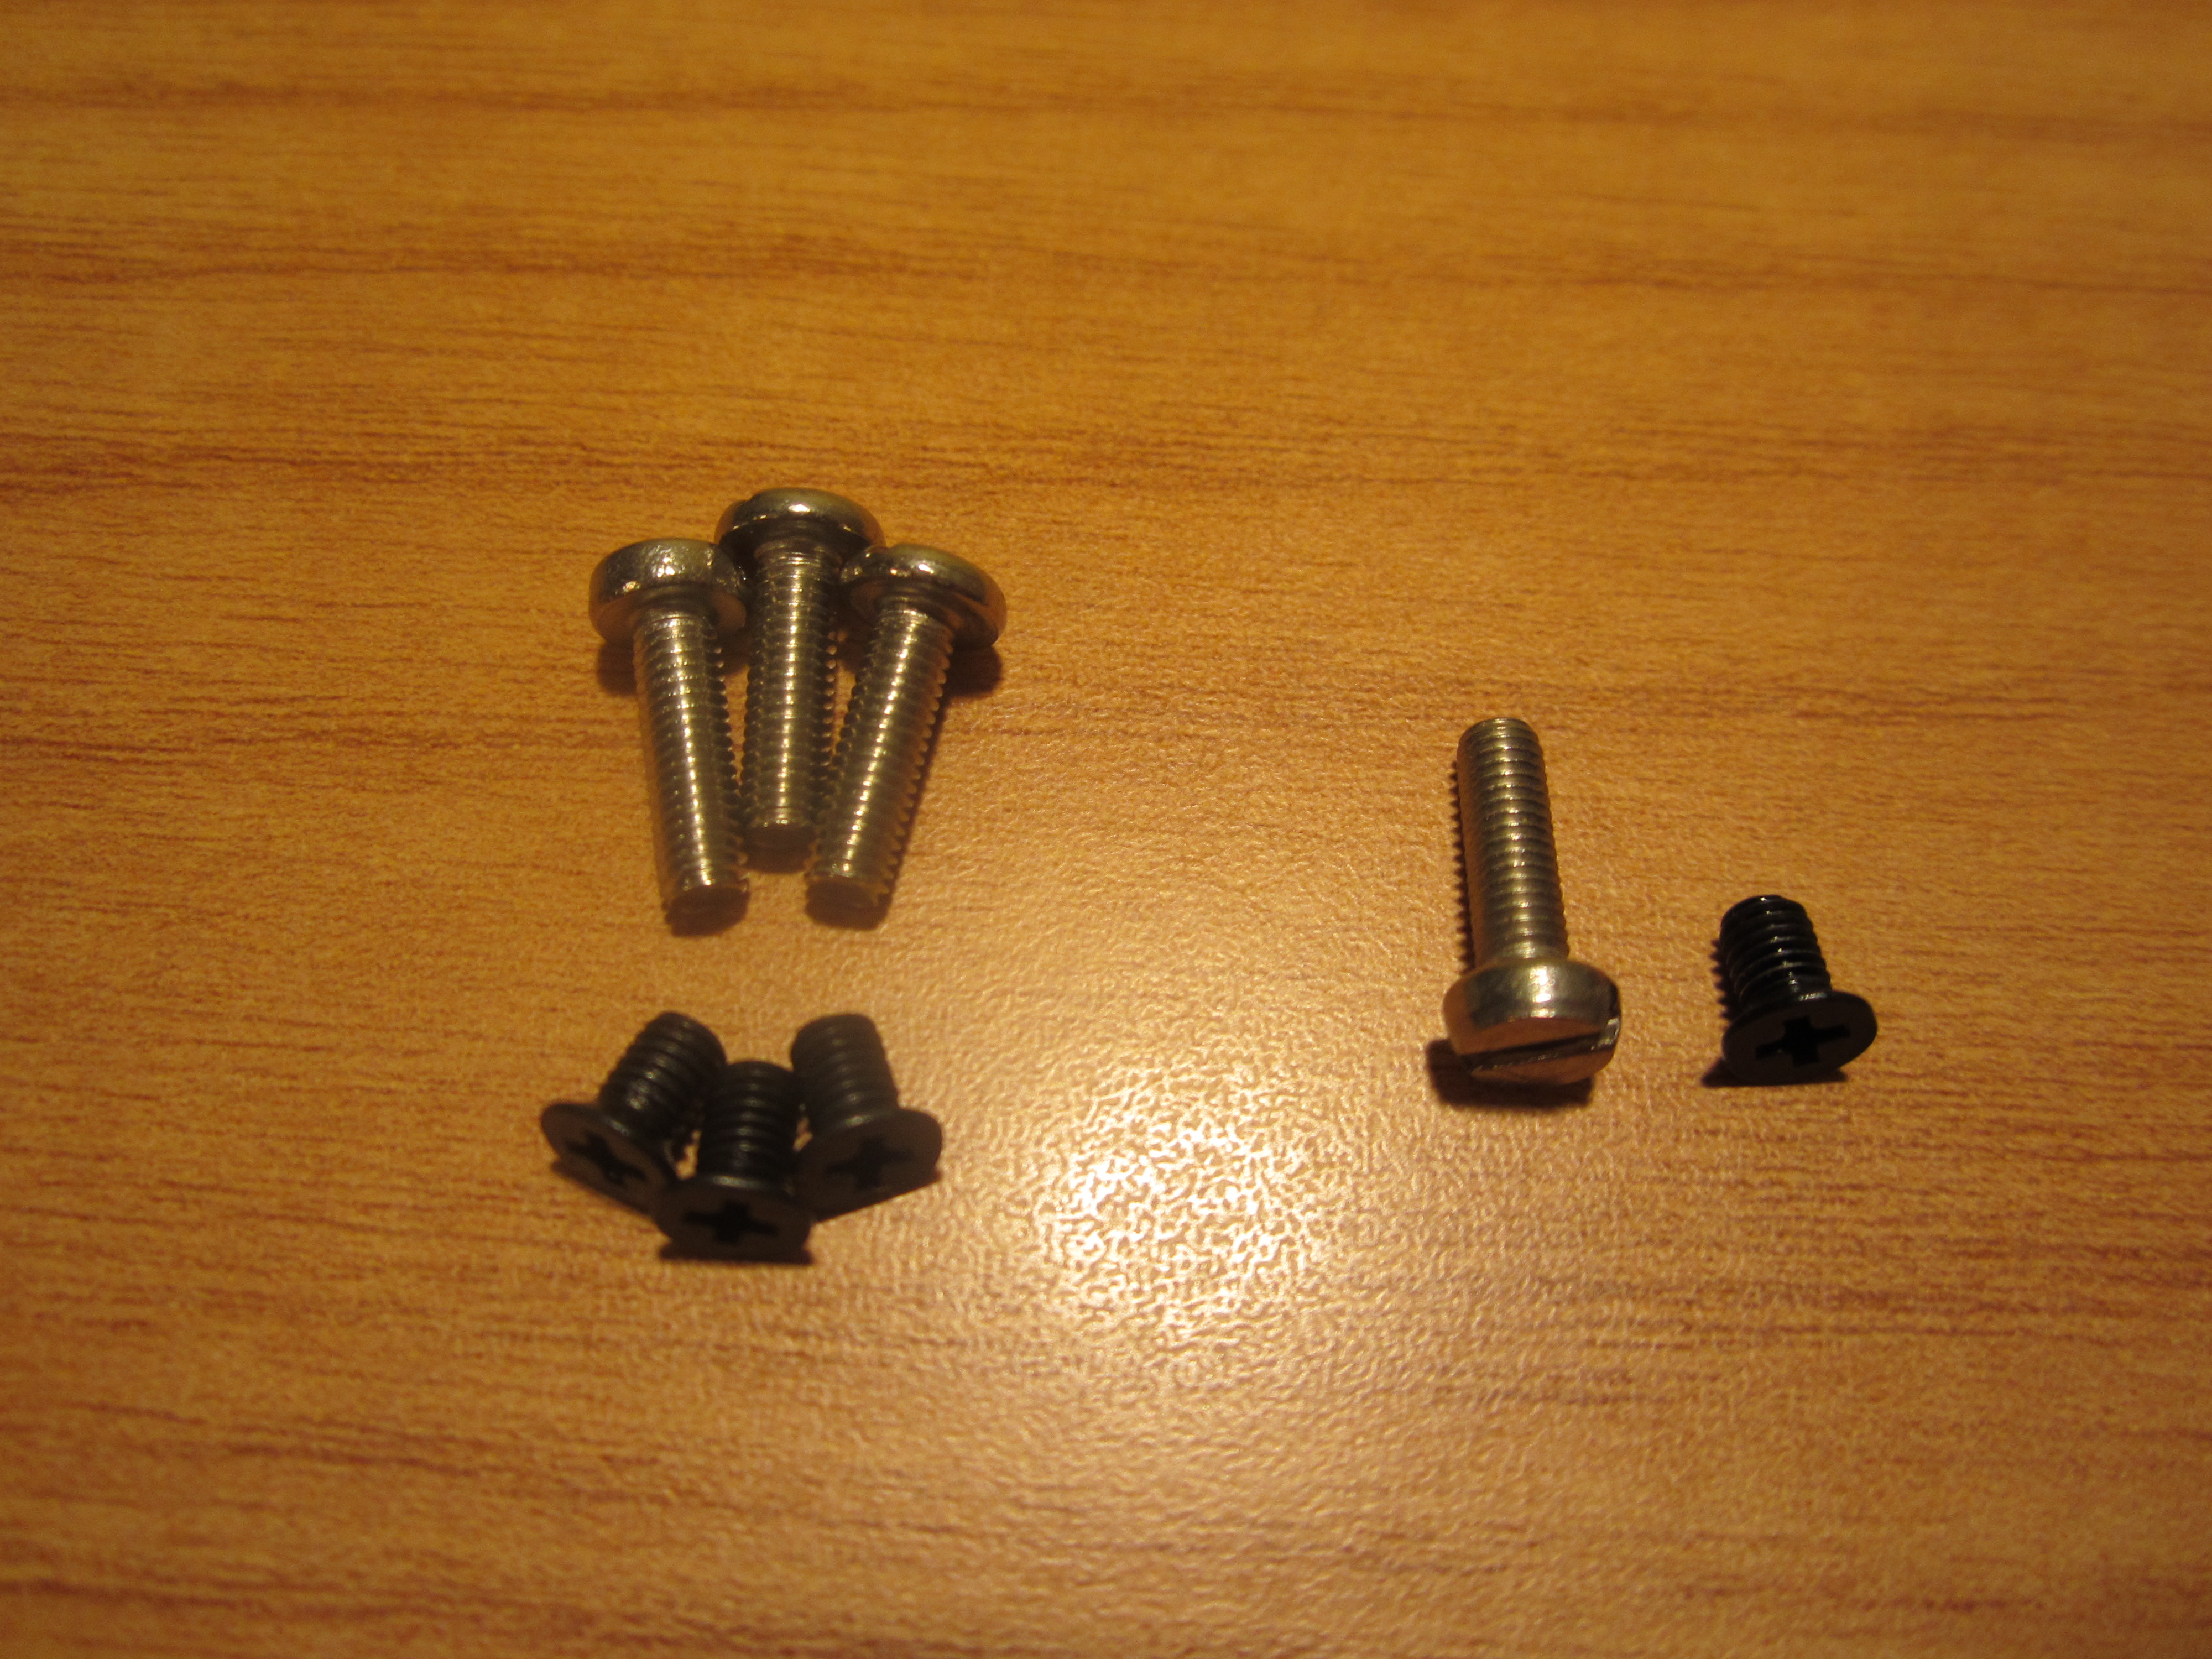
\includegraphics[width=0.8 \linewidth]{Images/Mounting/IMG_0342.jpg}}
\captionof{figure}{}% only if needed
\label{screwDifferences}
\end{minipage}    
\clearpage

We should note that the holes motors and arms are not equally spaced, so it is possible that when we screw a couple of screws fit and the rest not. To make sure they fit correctly, you must make the motor cables face the other end of the arm as you see in the figure below.

\noindent%
\begin{minipage}{\linewidth}
\vspace{10 mm}
\makebox[\linewidth]{%
  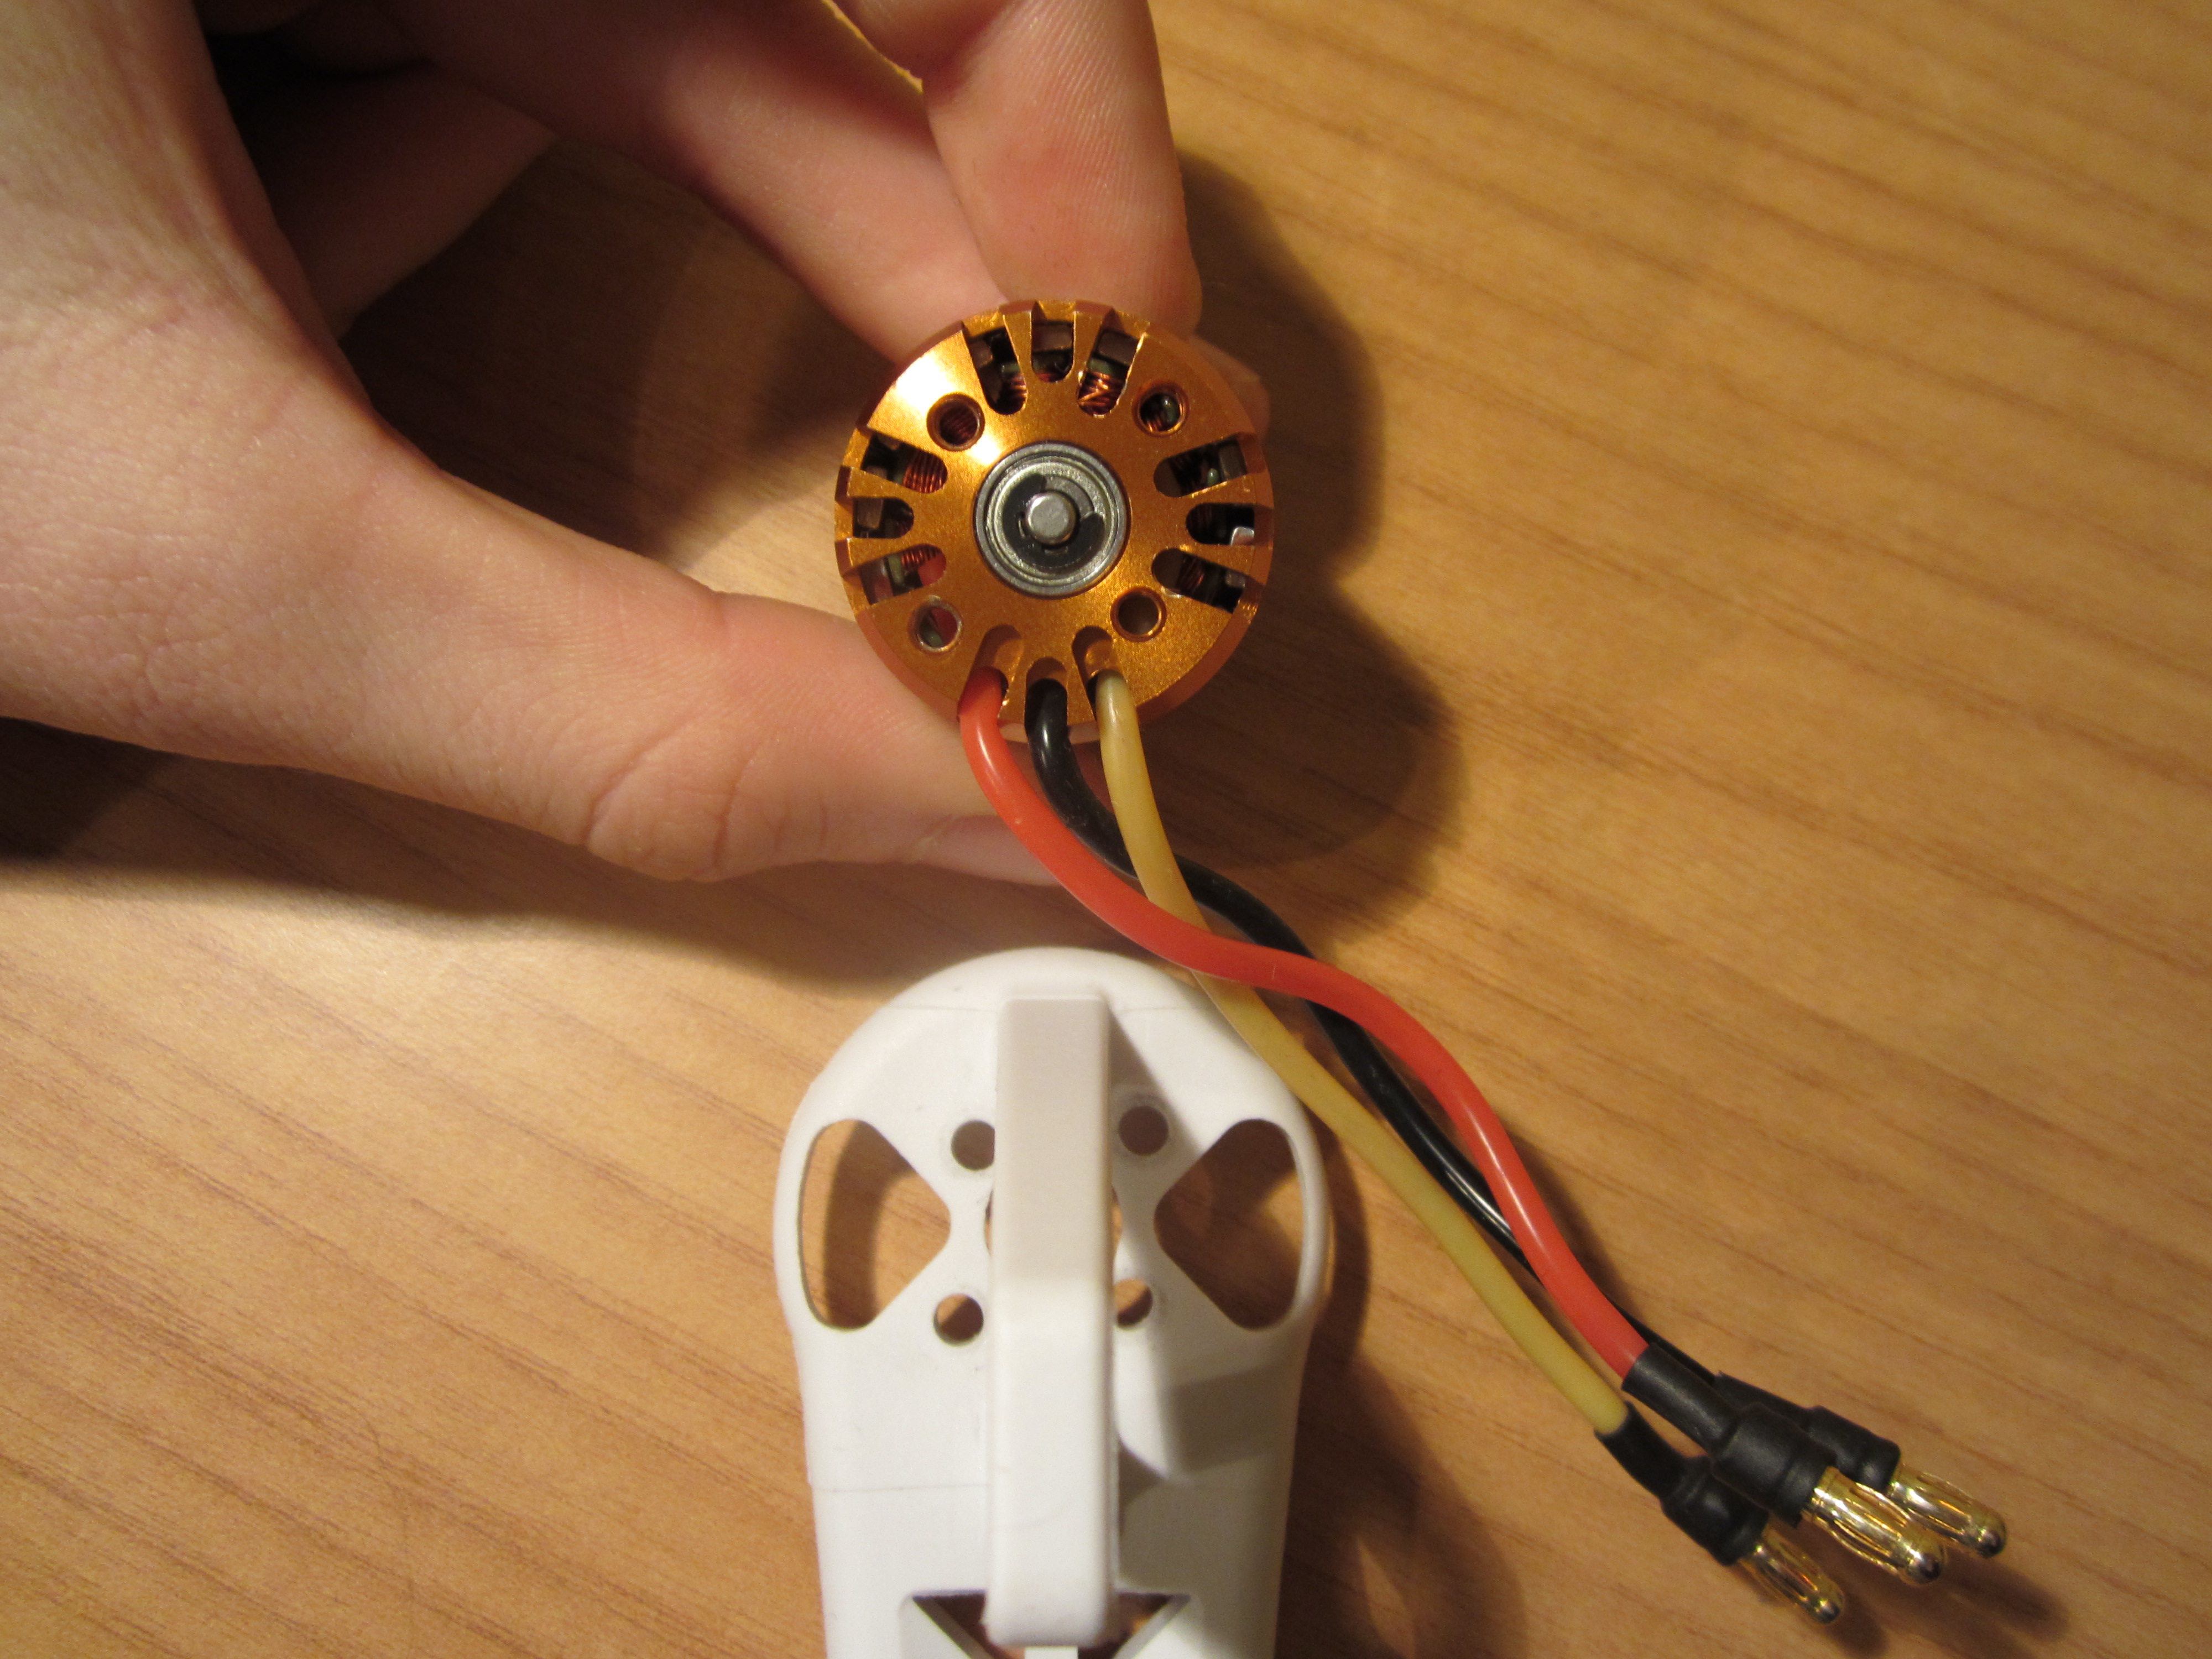
\includegraphics[width=0.8 \linewidth]{Images/Mounting/IMG_0446.jpg}}
\captionof{figure}{}% only if needed
\label{motorArm}
\end{minipage}    
\\[12pt]

As a tip, first screw the screws located diagonally in order to strengthen the position. This allows you to screw in a more convenient and simple way the rest.
\\[12pt]

\begin{minipage}{0.5\textwidth}
  \centering
  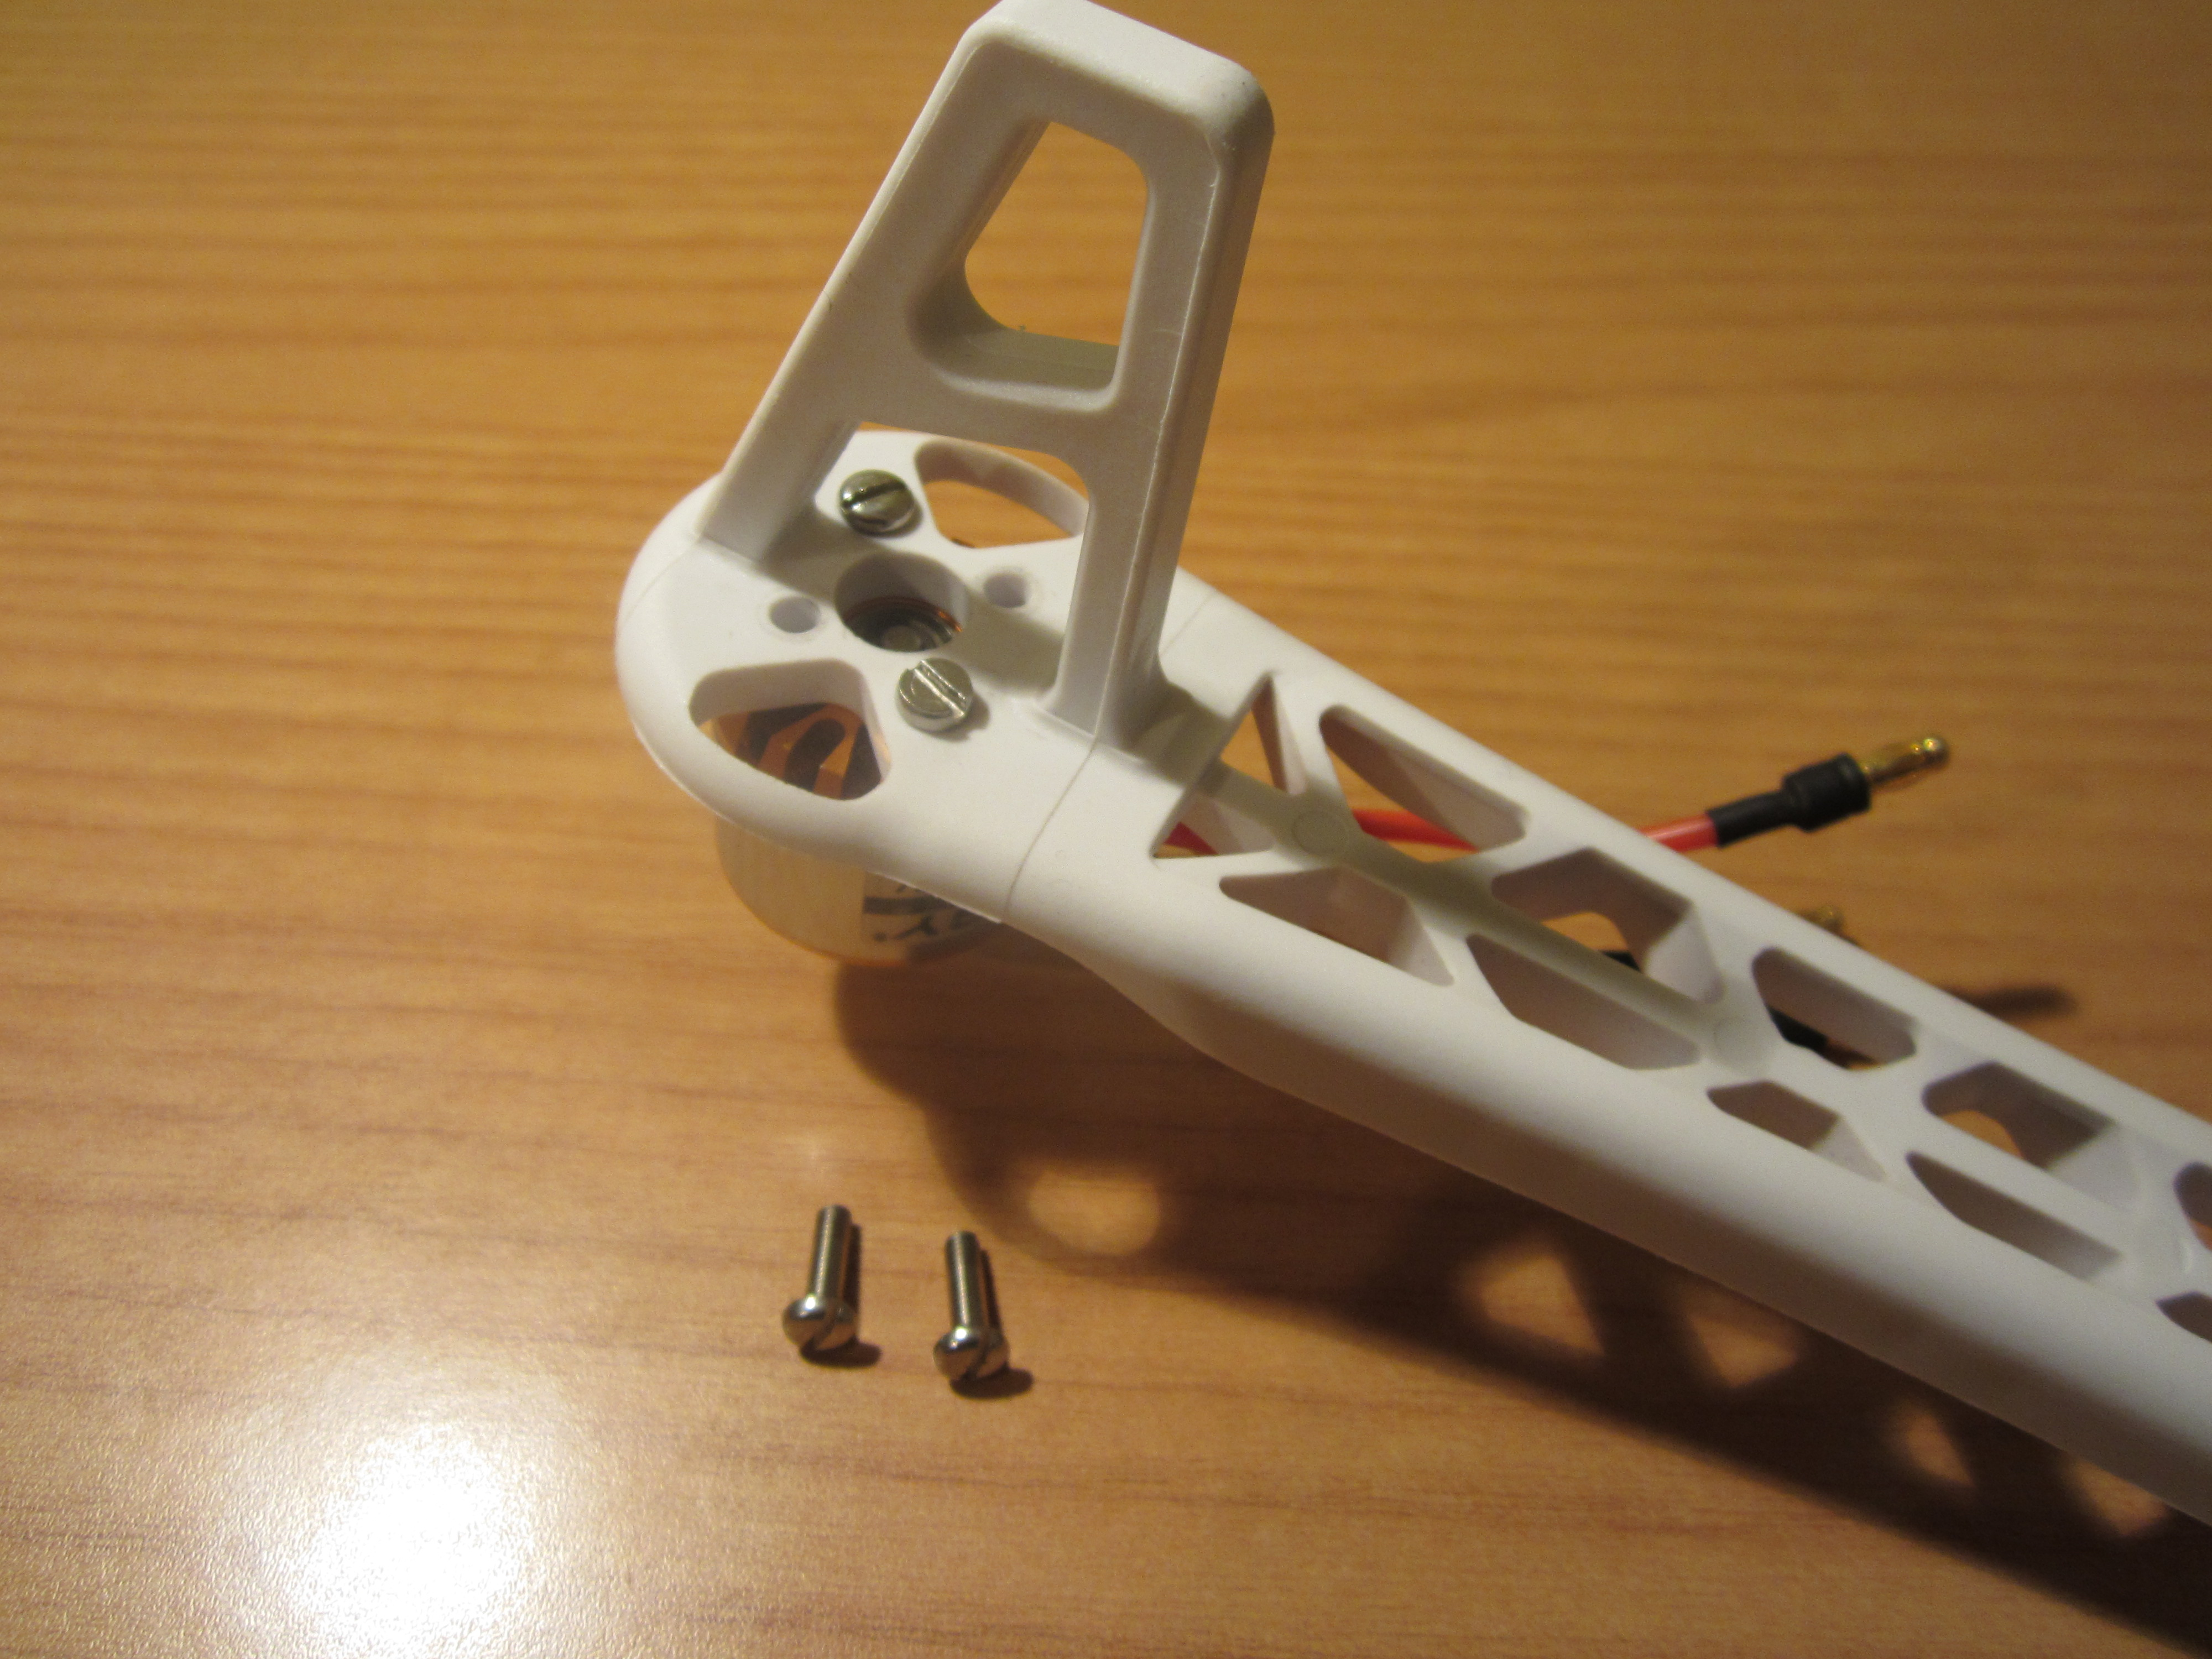
\includegraphics[width=0.8\linewidth]{Images/Mounting/IMG_0449.jpg}
  \captionof{figure}{}
  \label{diagScrews}
\end{minipage}%
\begin{minipage}{0.5\textwidth}
  \centering
  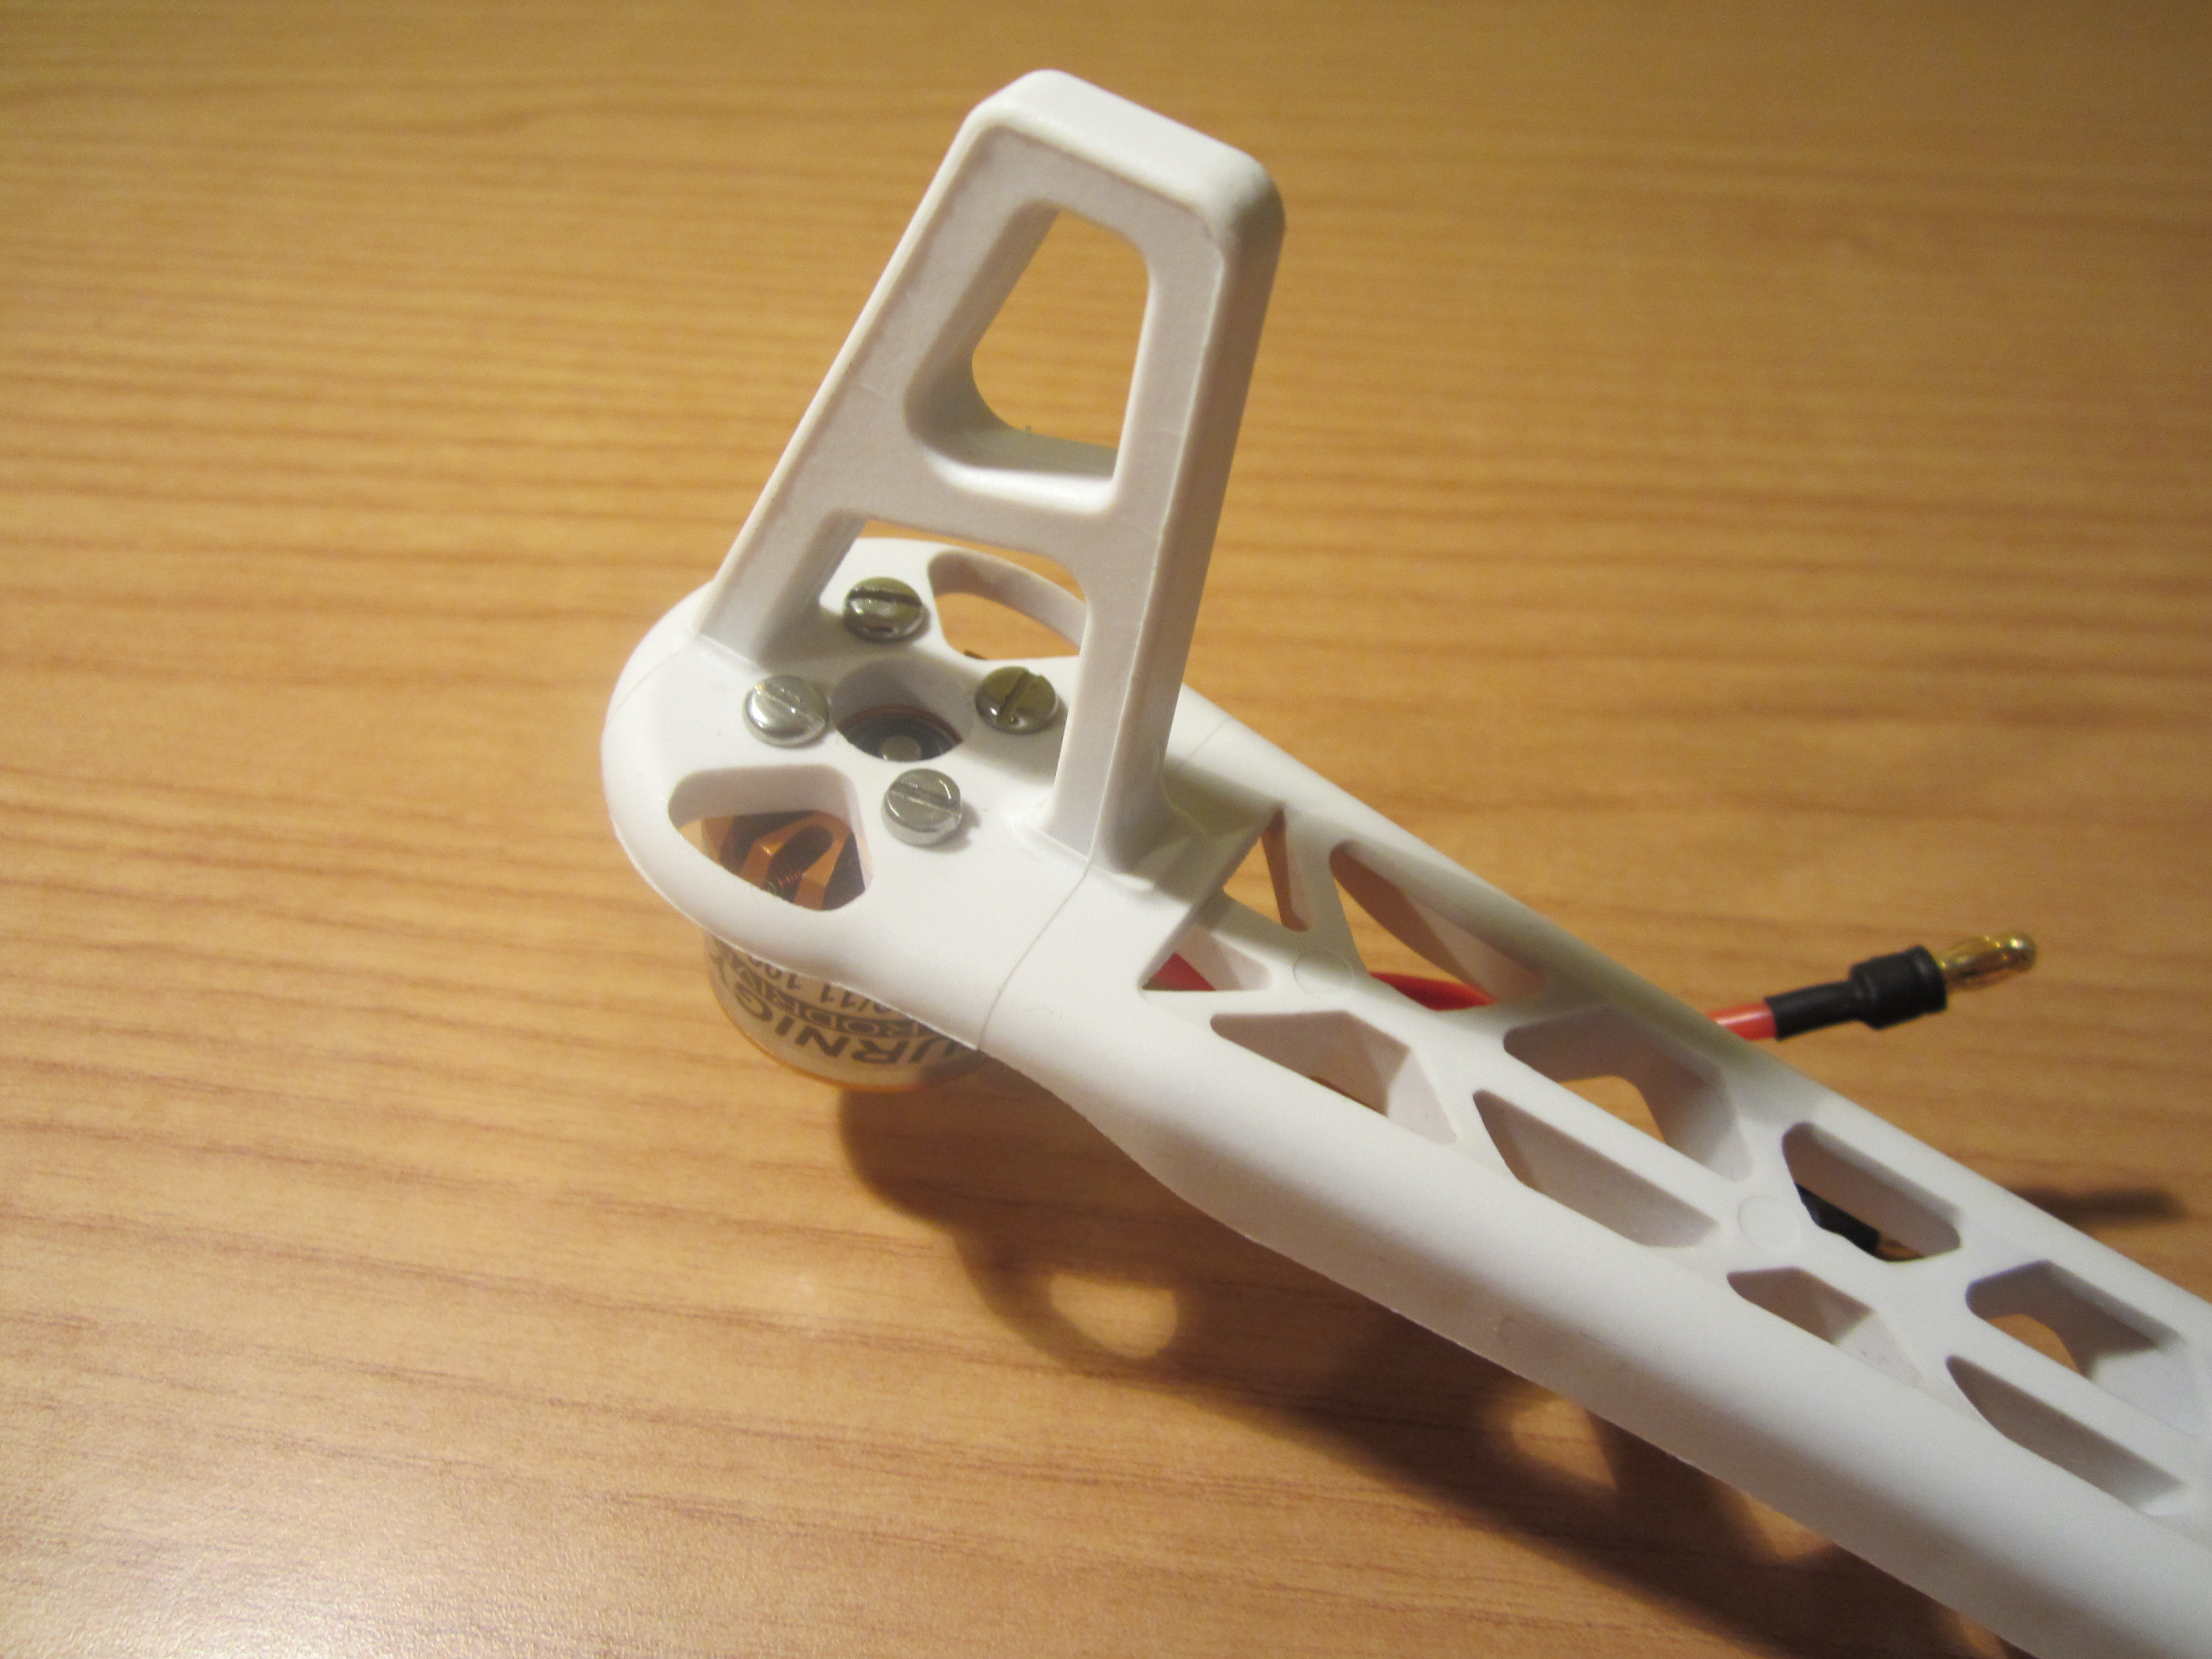
\includegraphics[width=0.8\linewidth]{Images/Mounting/IMG_0450.jpg}
  \captionof{figure}{}
  \label{allScrews}
\end{minipage}
\\[12pt]
\clearpage

If now we set the propeller on the motor we can see how they stand out a bit. This fact is not very important, however, it is recommended to trim the iron bar of about 0.5cm, so they are closer together.
\\[12pt]

\begin{minipage}{0.5\textwidth}
  \centering
  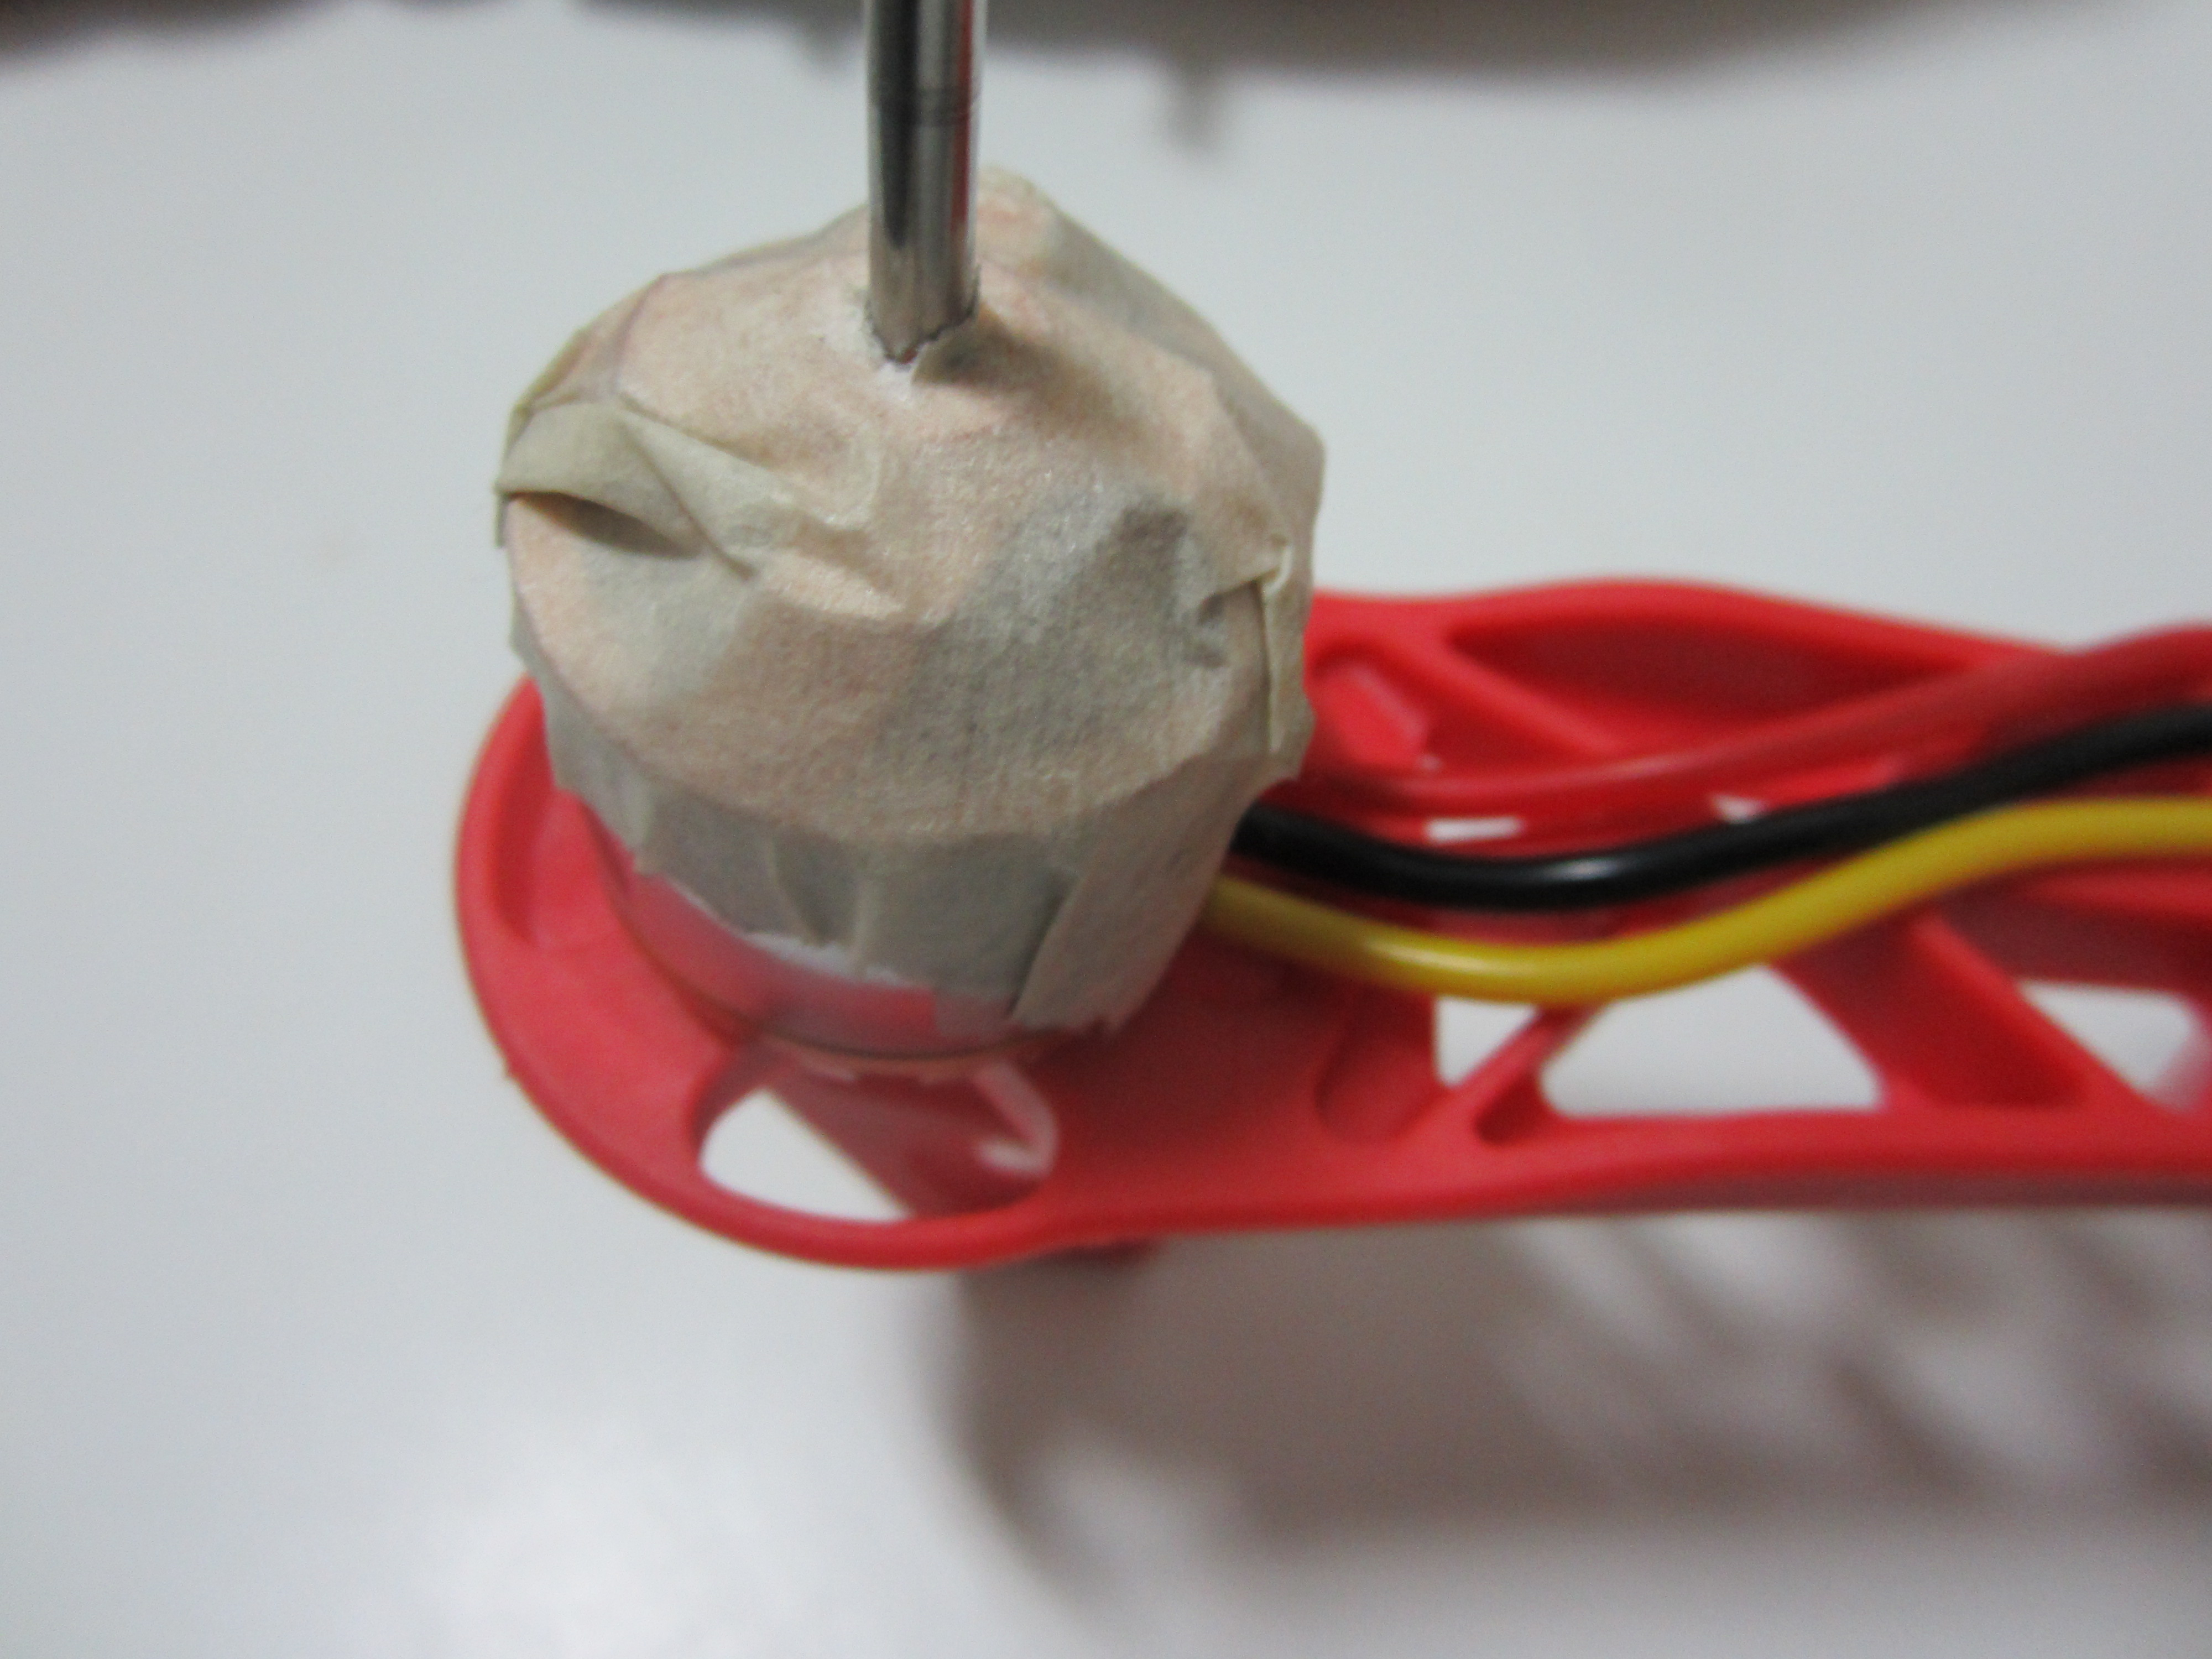
\includegraphics[width=0.8\linewidth]{Images/Mounting/IMG_0432.jpg}
  \captionof{figure}{}
  \label{fig:app1}
\end{minipage}%
\begin{minipage}{0.5\textwidth}
  \centering
  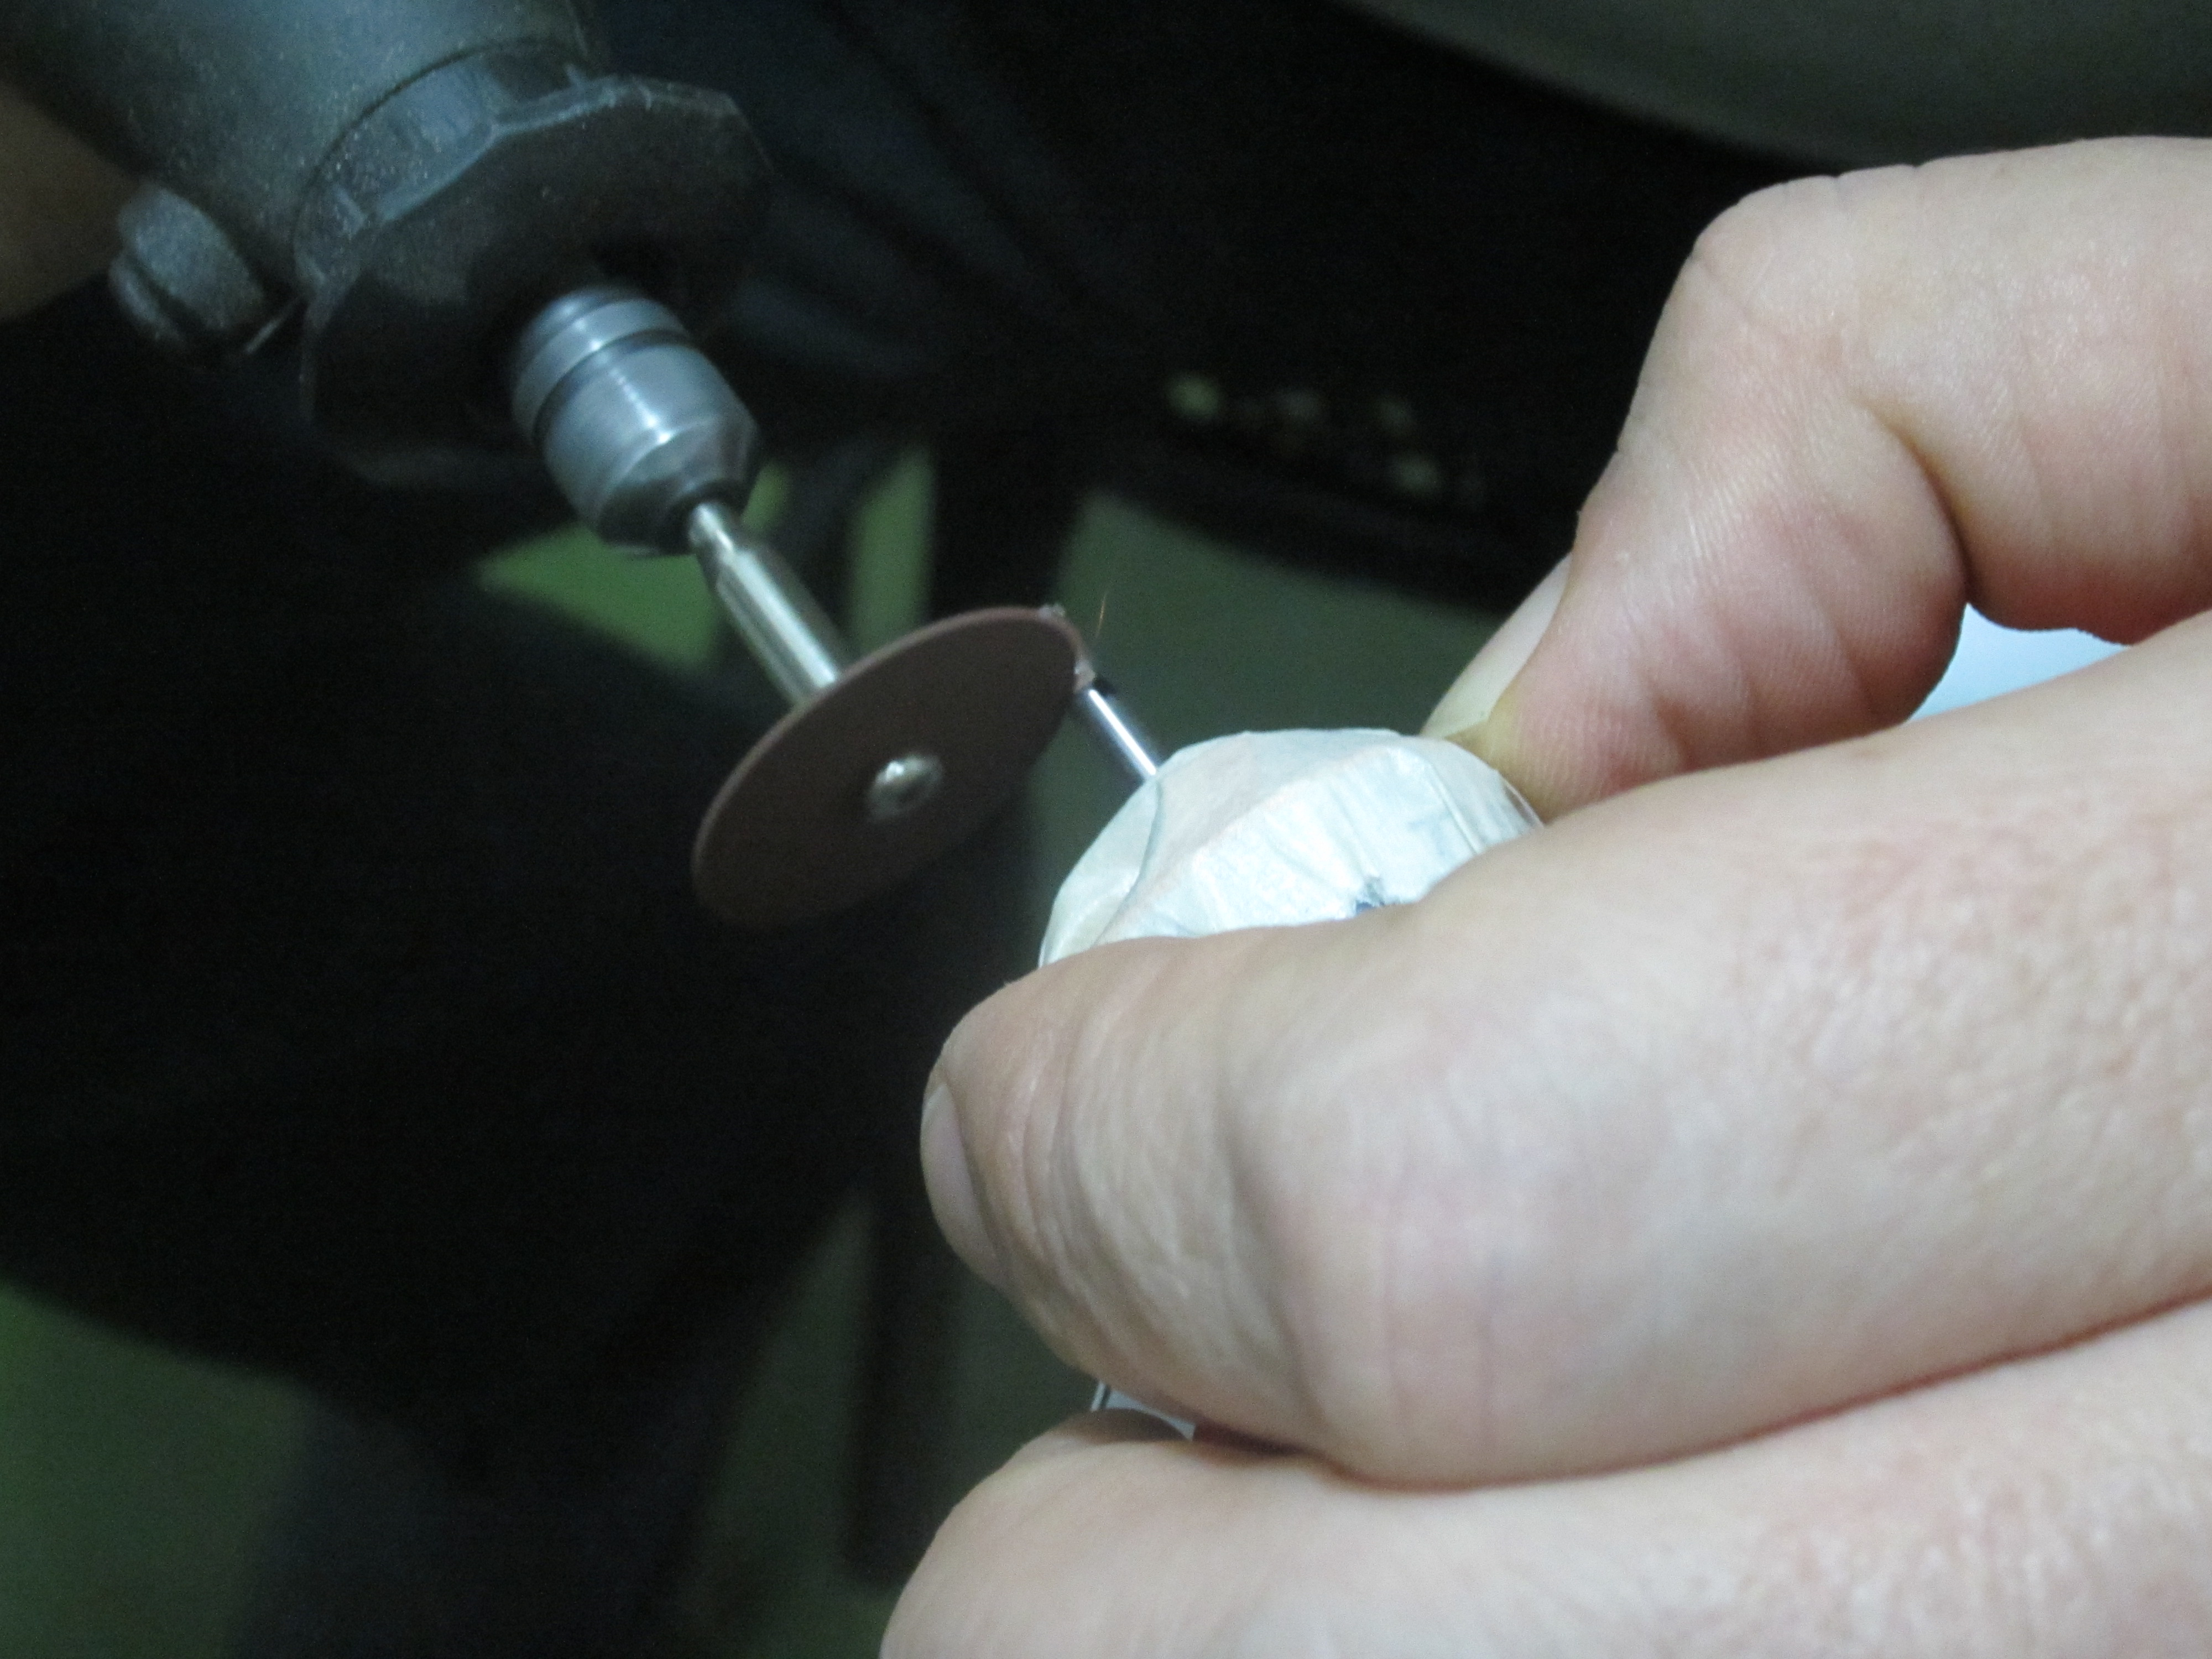
\includegraphics[width=0.8\linewidth]{Images/Mounting/IMG_0435.jpg}
  \captionof{figure}{}
  \label{fig:app2}
\end{minipage}

To perform this task we protect the engine from scrap when we cut, so it is recommended to drill a paper with iron or tape to cover the motor and prevent damage.

\noindent%
\begin{minipage}{\linewidth}
\vspace{10 mm}
\makebox[\linewidth]{%
  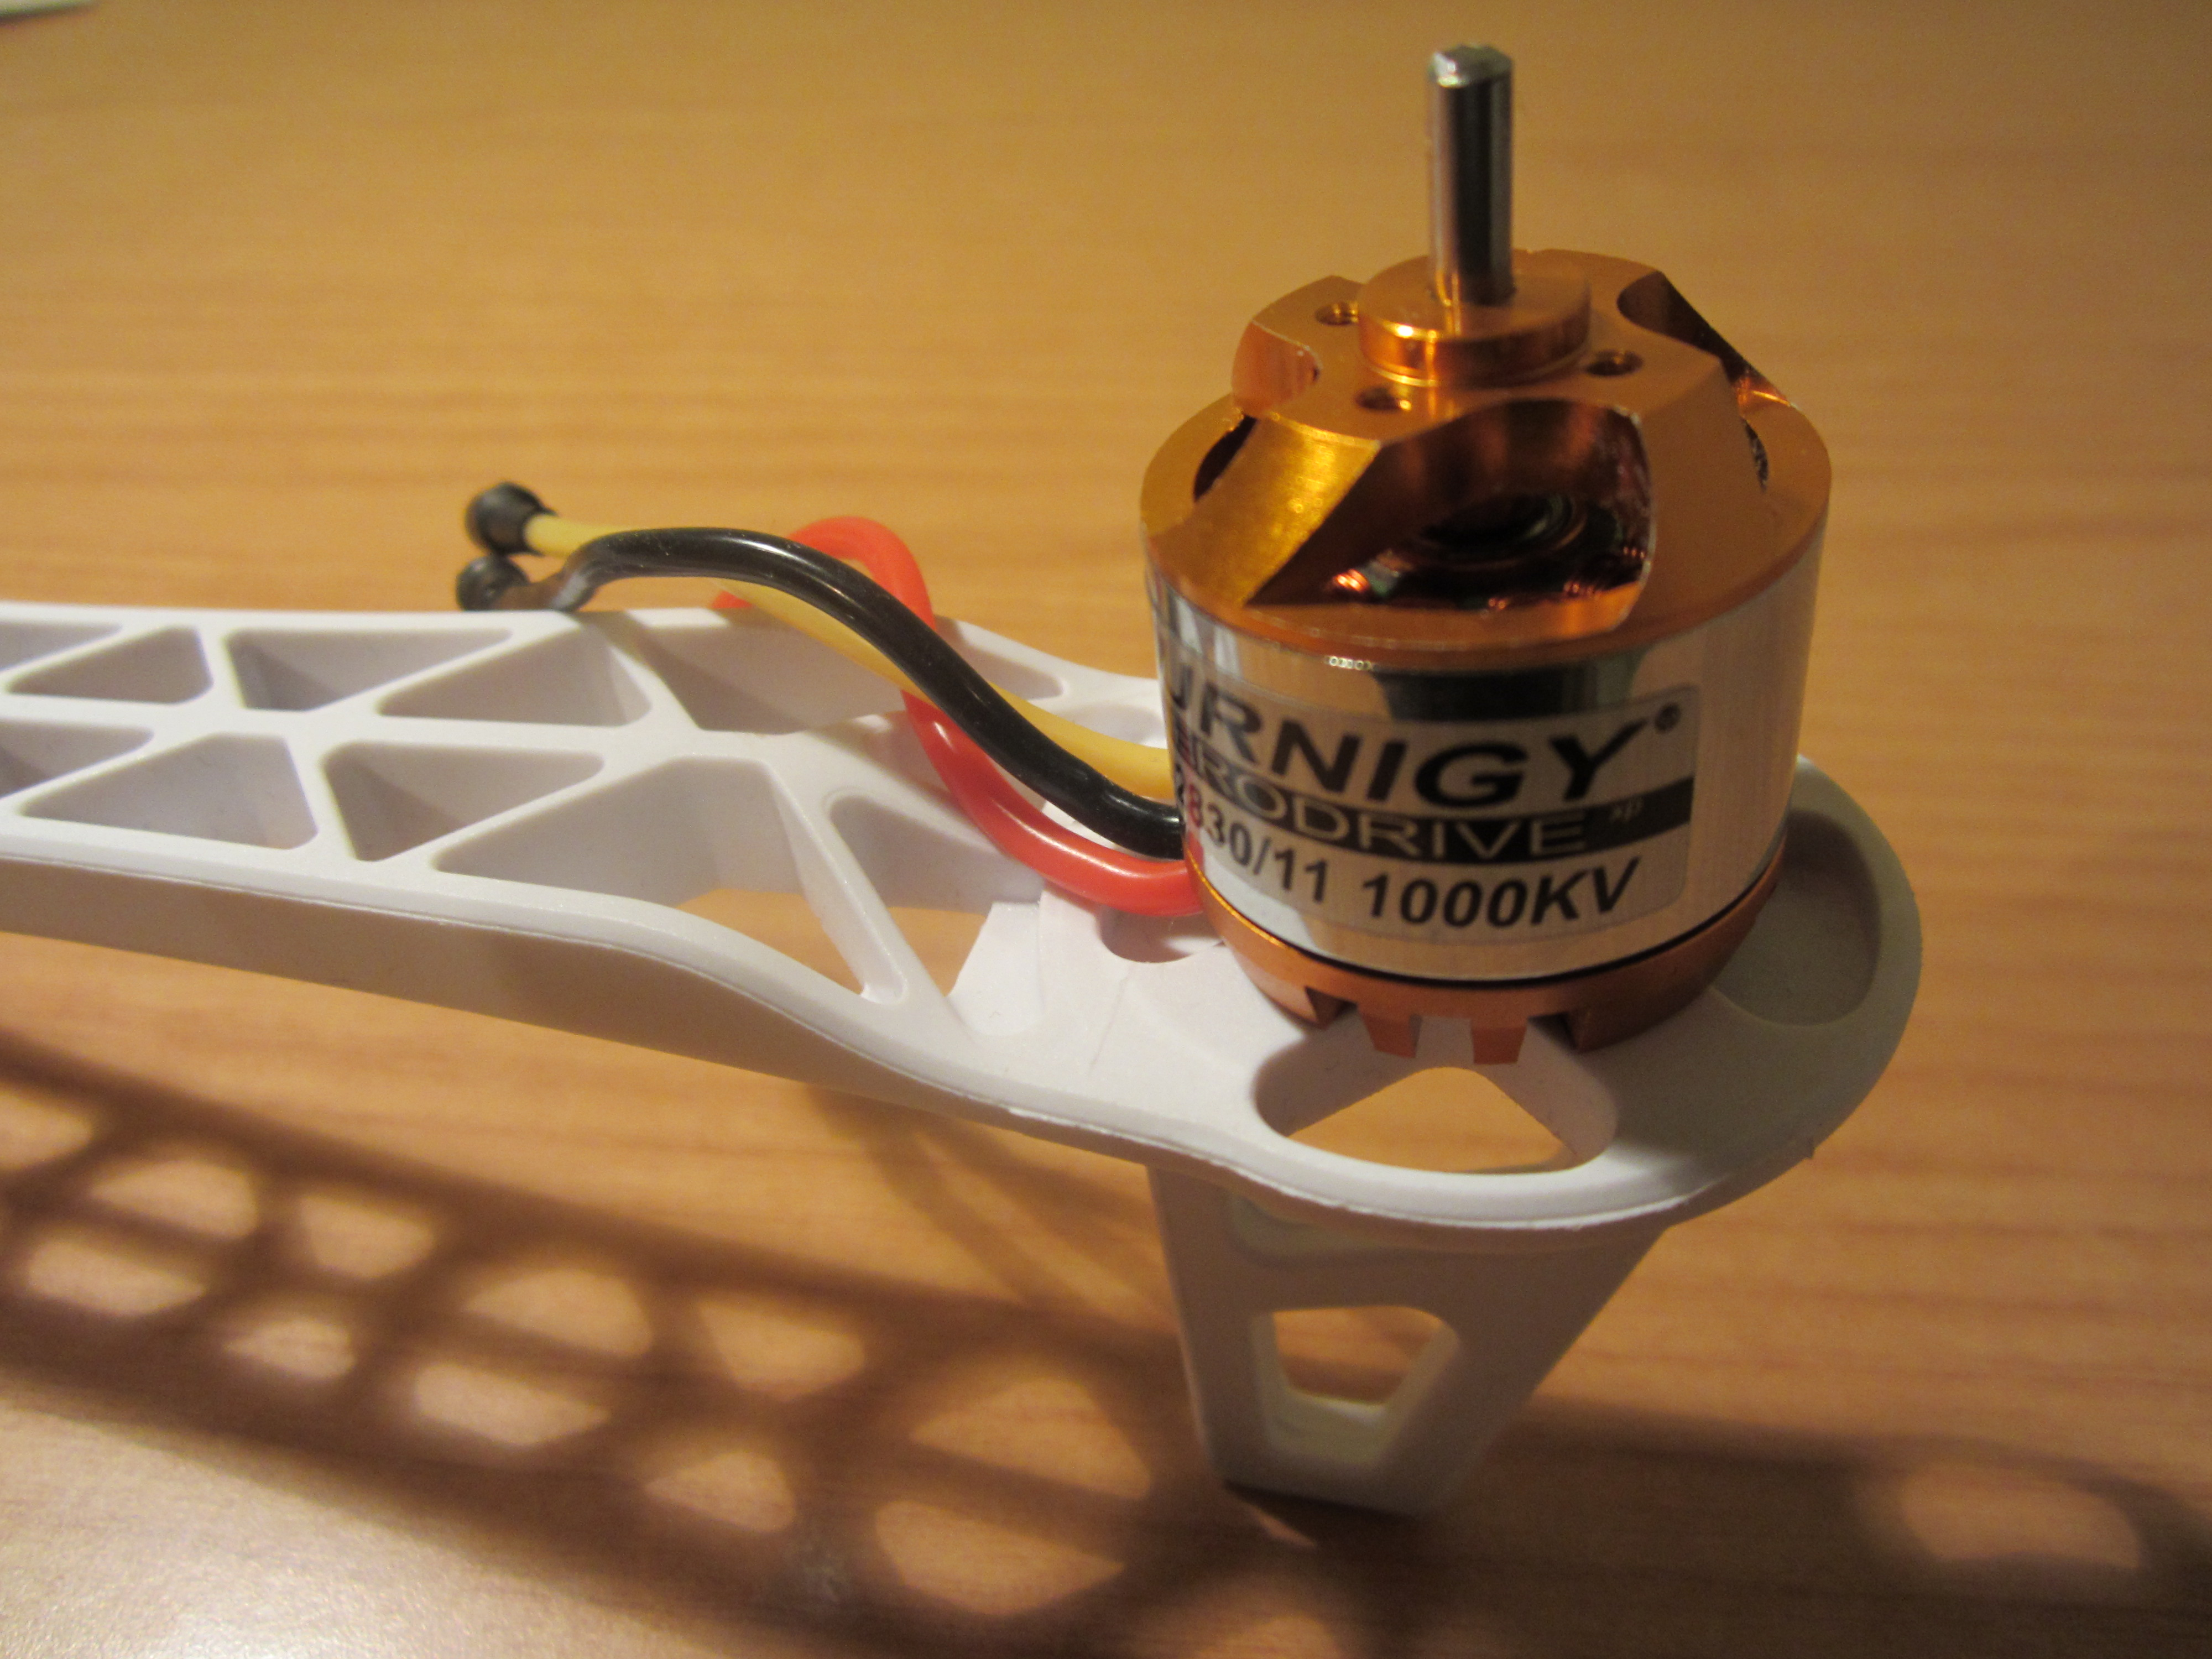
\includegraphics[width=0.8 \linewidth]{Images/Mounting/IMG_0452.jpg}}
\captionof{figure}{}% only if needed
\label{mobilenode1}
\end{minipage}    


\section{Base solders}

The wiring that connects the ESC to the base is too long, so it is recommended to cut the remaining wiring. This cut is approximately 1.5cm excluding the connector. After that, do not forget about to peel 0.5cm of cable in order to solder it correctly.
\\[12 pt]

\begin{minipage}{0.5\textwidth}
  \centering
  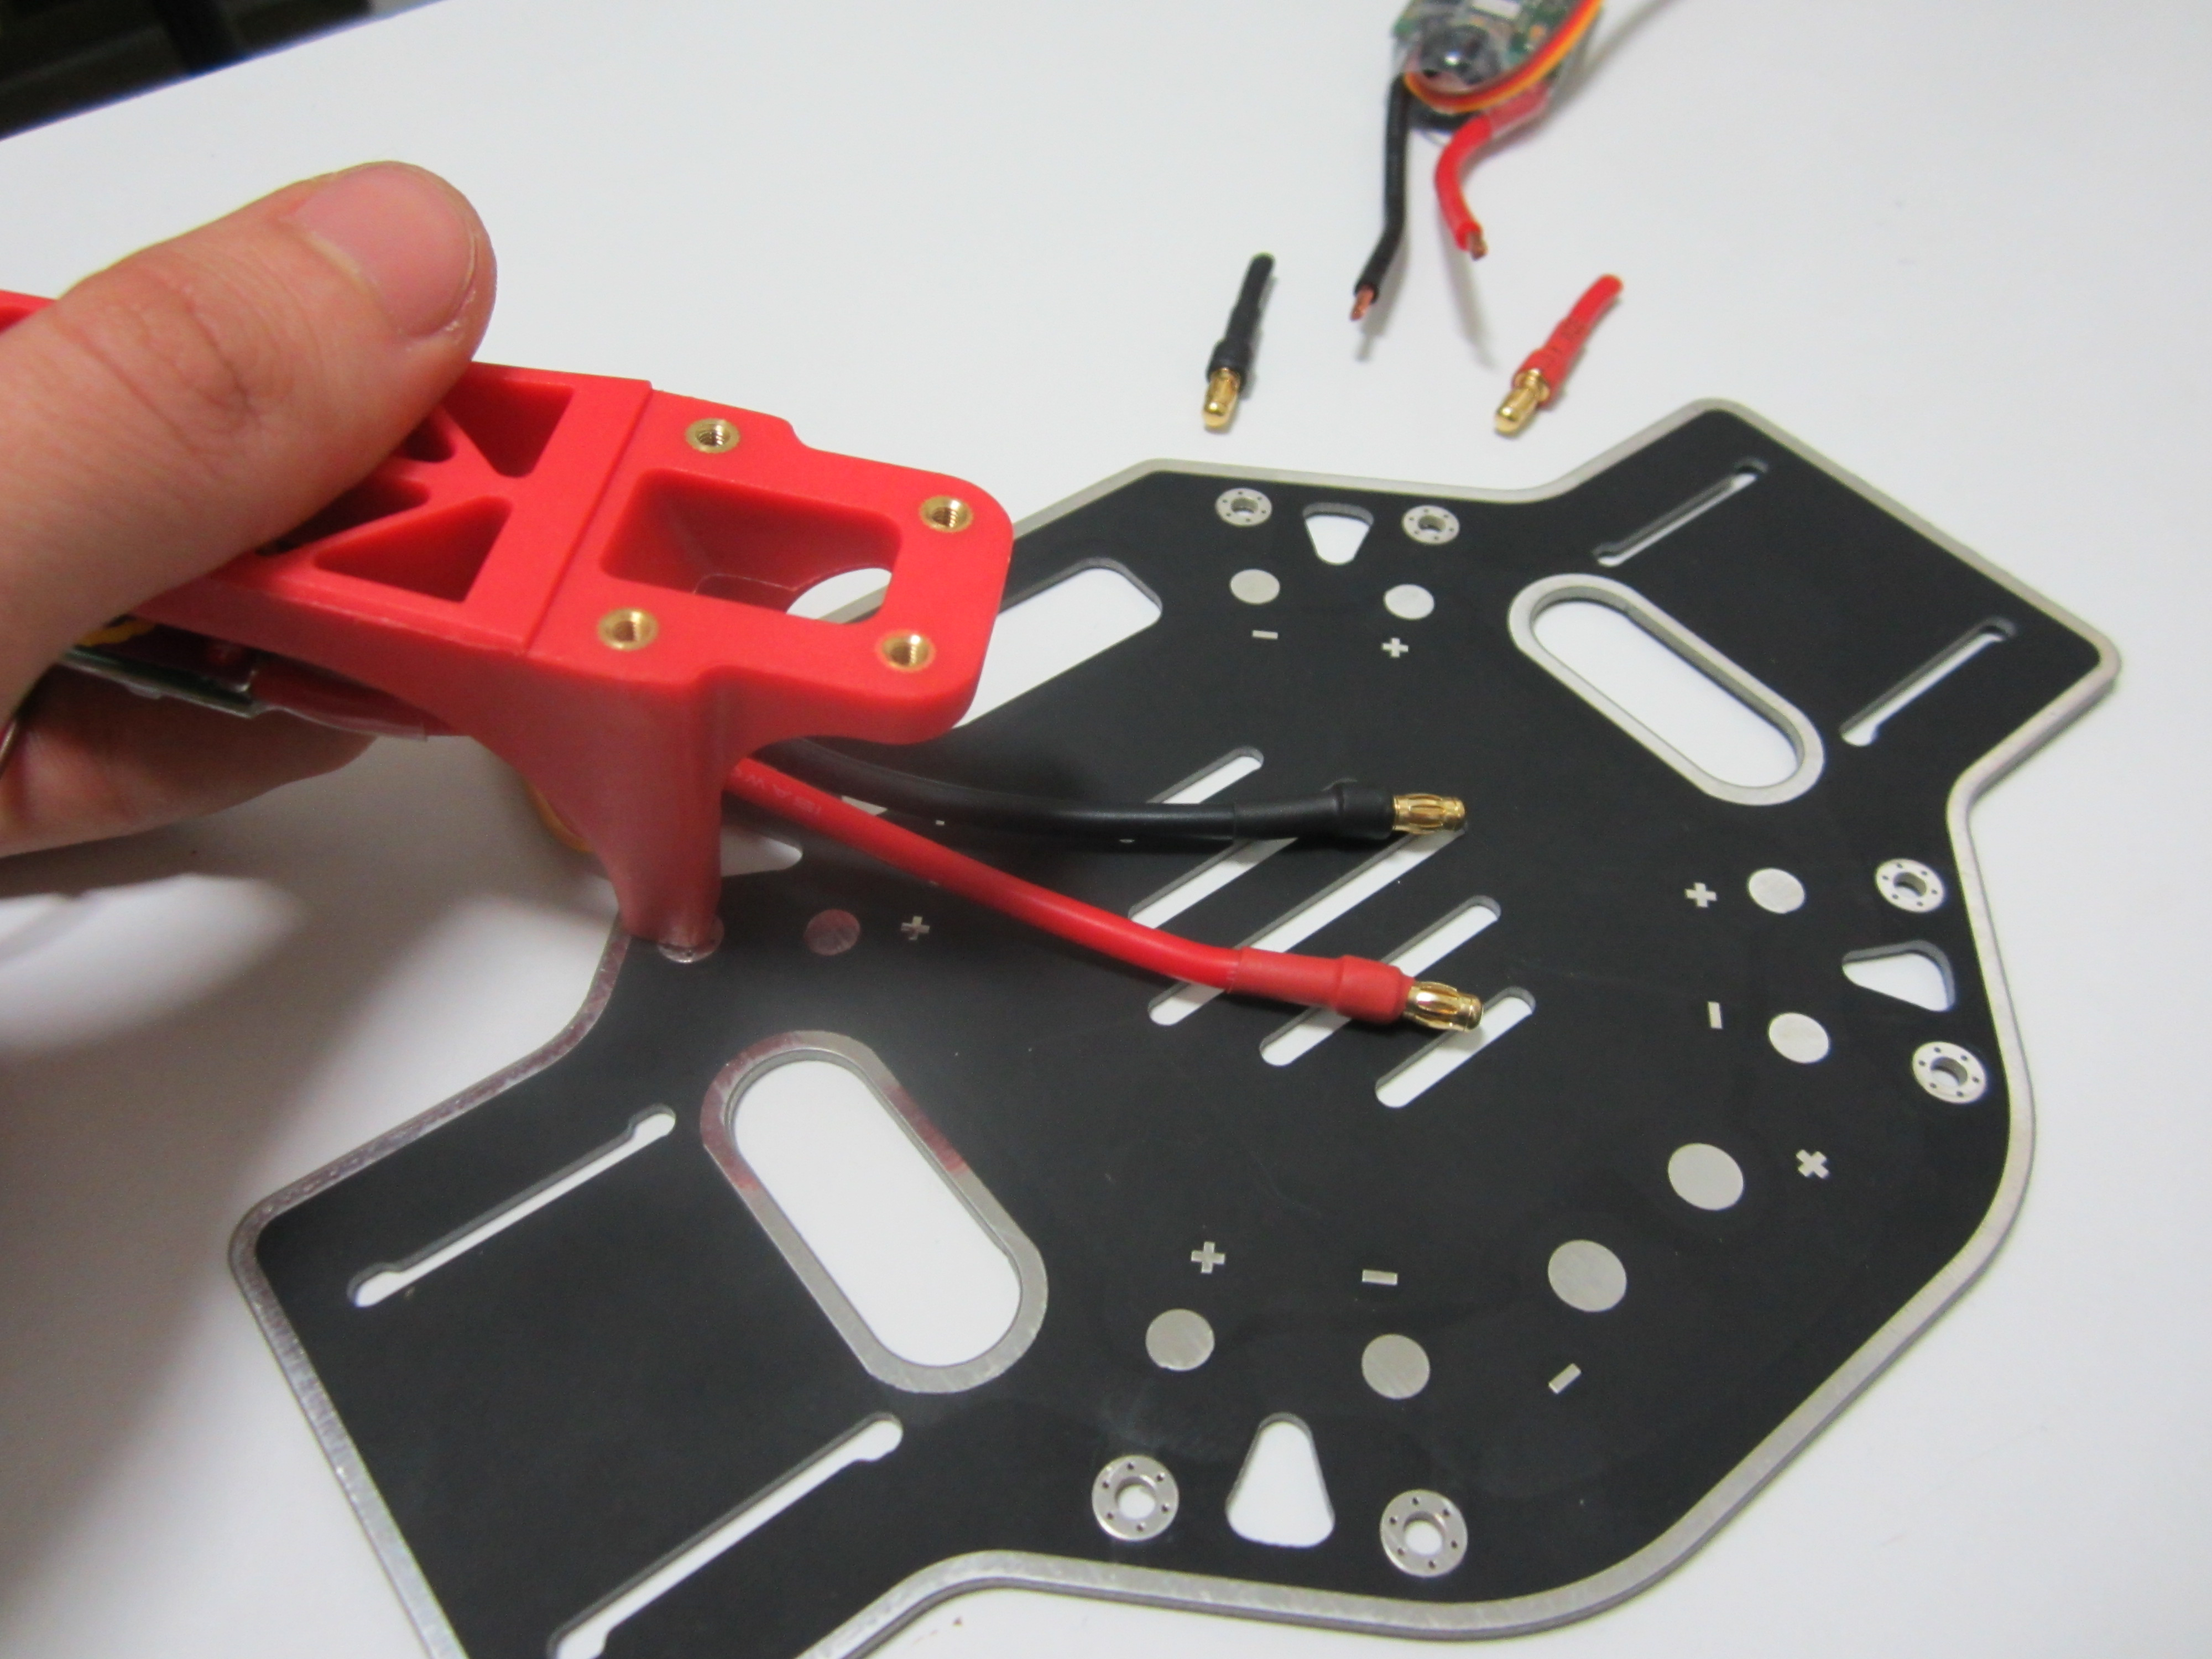
\includegraphics[width=0.8\linewidth]{Images/Mounting/IMG_0366.jpg}
  \captionof{figure}{}
  \label{fig:app1}
\end{minipage}%
\begin{minipage}{0.5\textwidth}
  \centering
  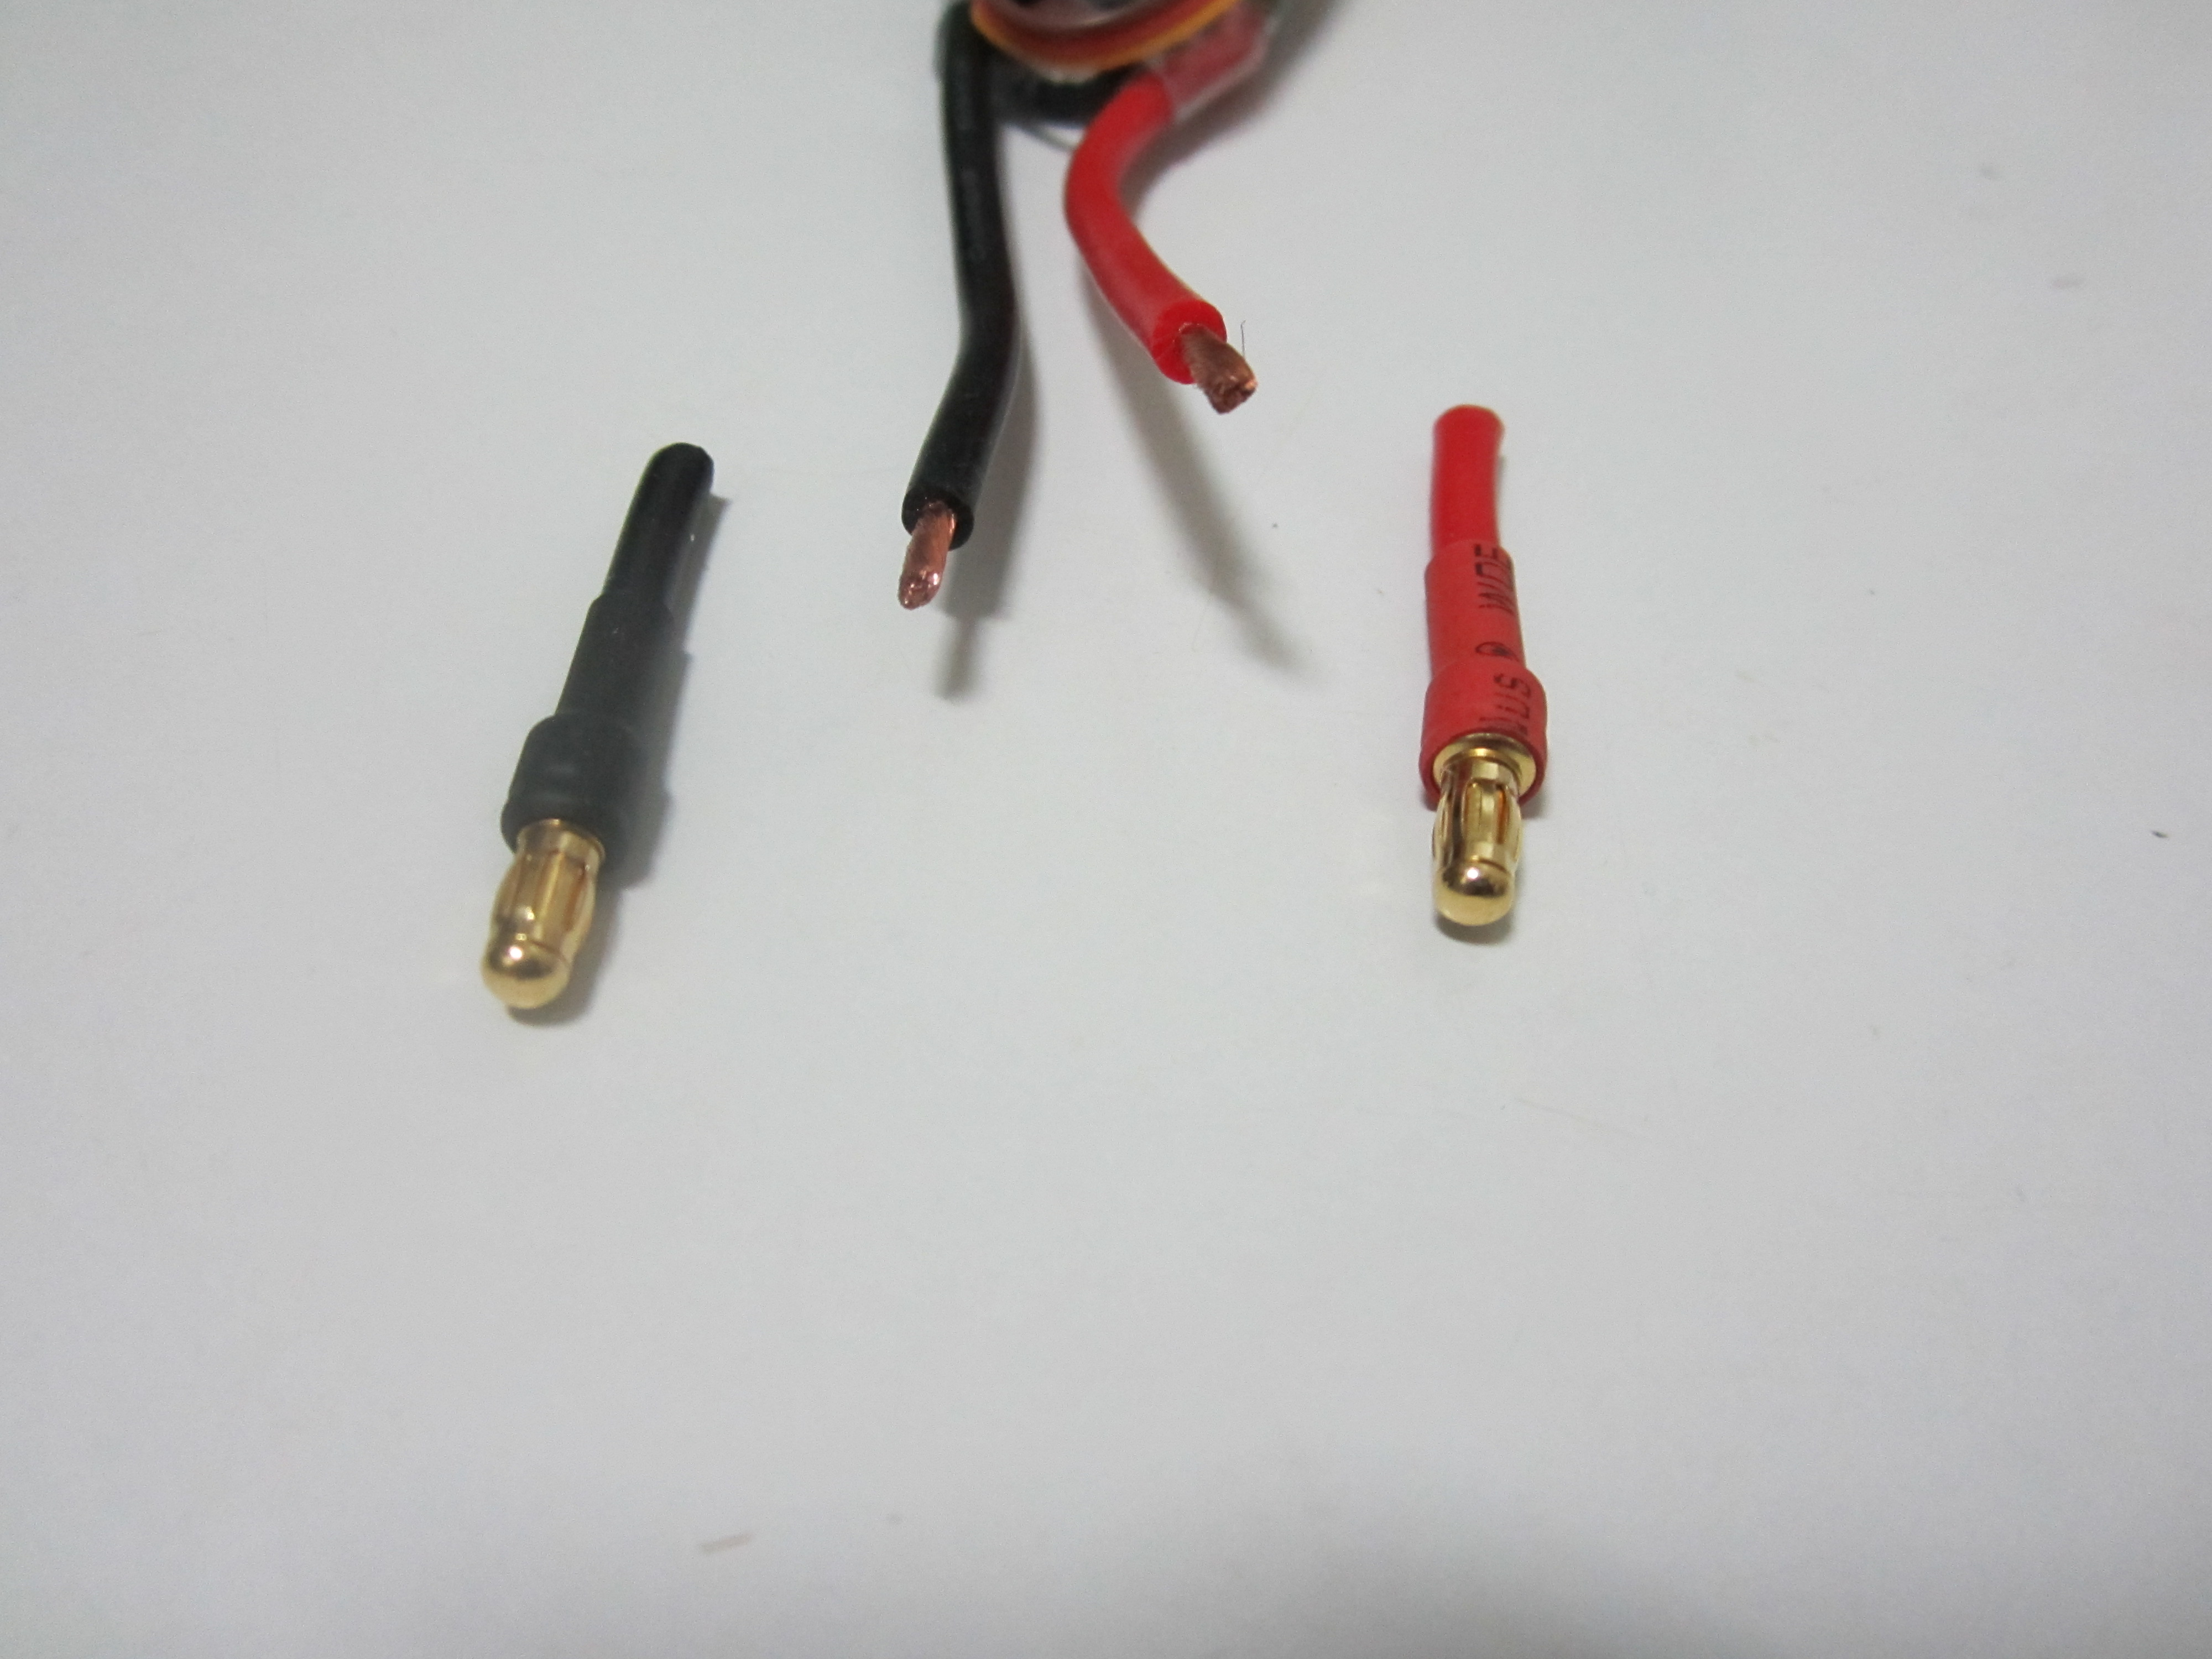
\includegraphics[width=0.8\linewidth]{Images/Mounting/IMG_0368.jpg}
  \captionof{figure}{}
  \label{fig:app2}
\end{minipage}


Soldering process
\\[12 pt]

\begin{minipage}{0.5\textwidth}
  \centering
  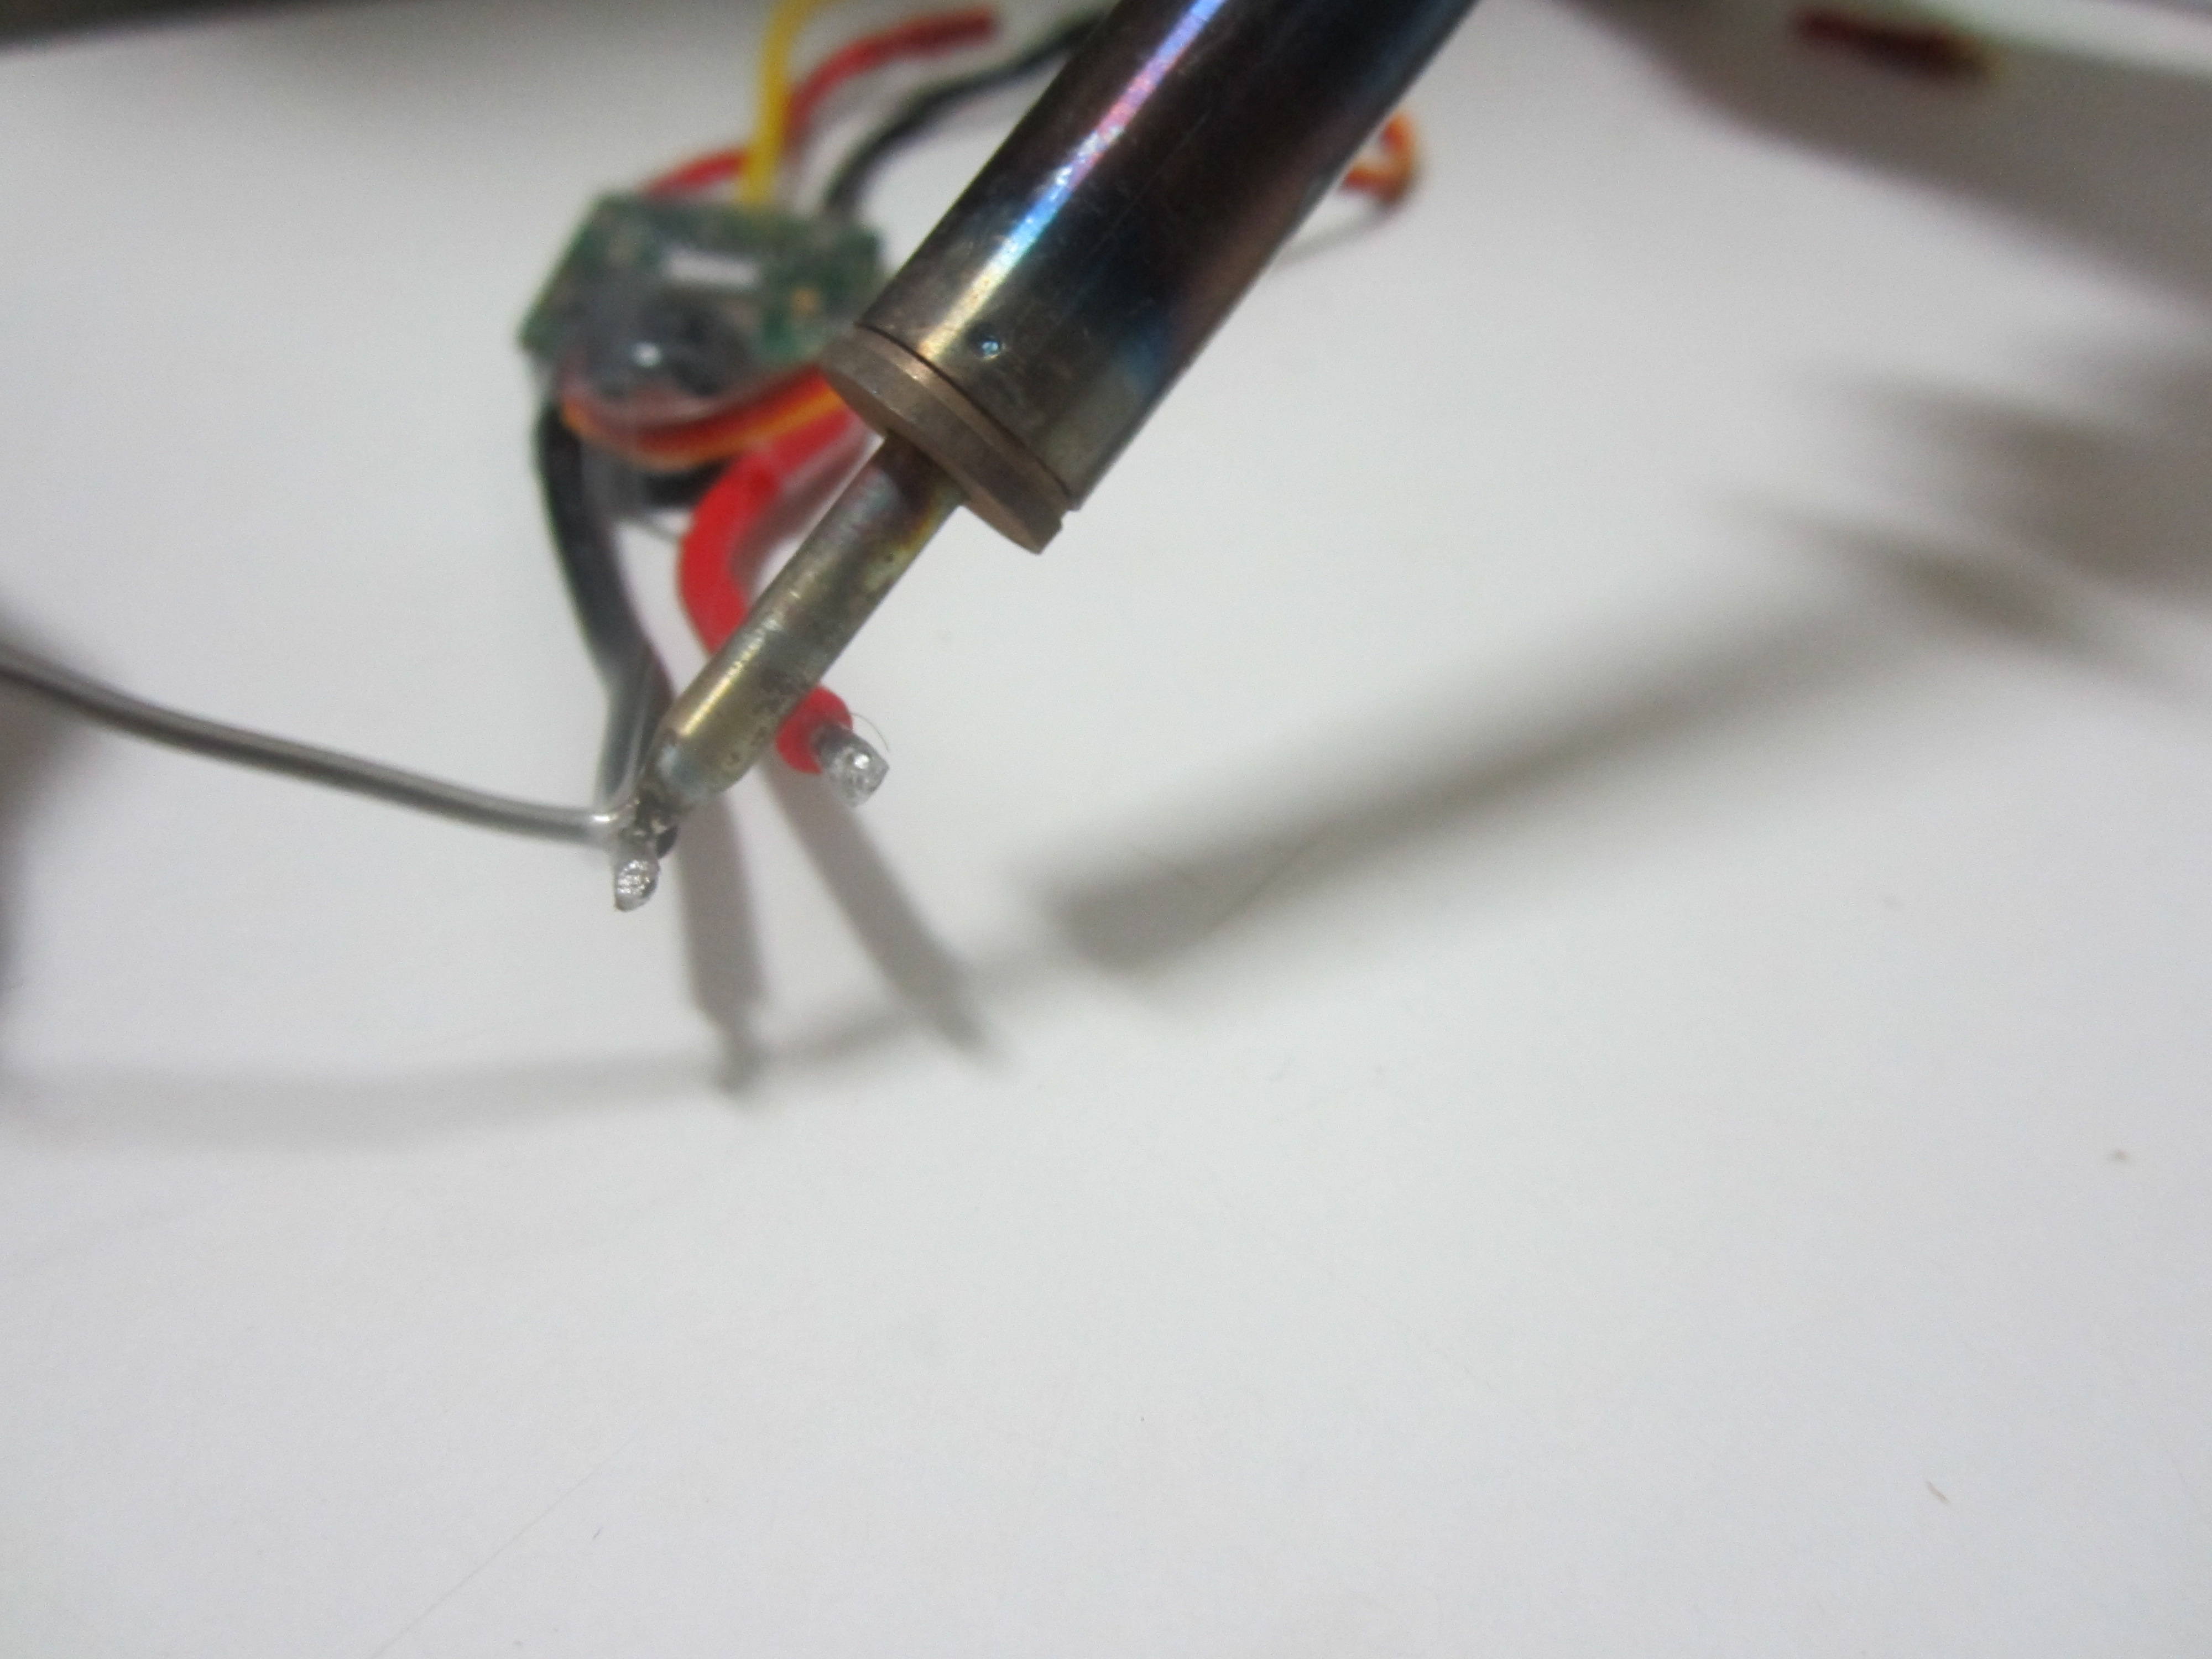
\includegraphics[width=0.8\linewidth]{Images/Mounting/IMG_0371.jpg}
  \captionof{figure}{}
  \label{fig:app1}
\end{minipage}%
\begin{minipage}{0.5\textwidth}
  \centering
  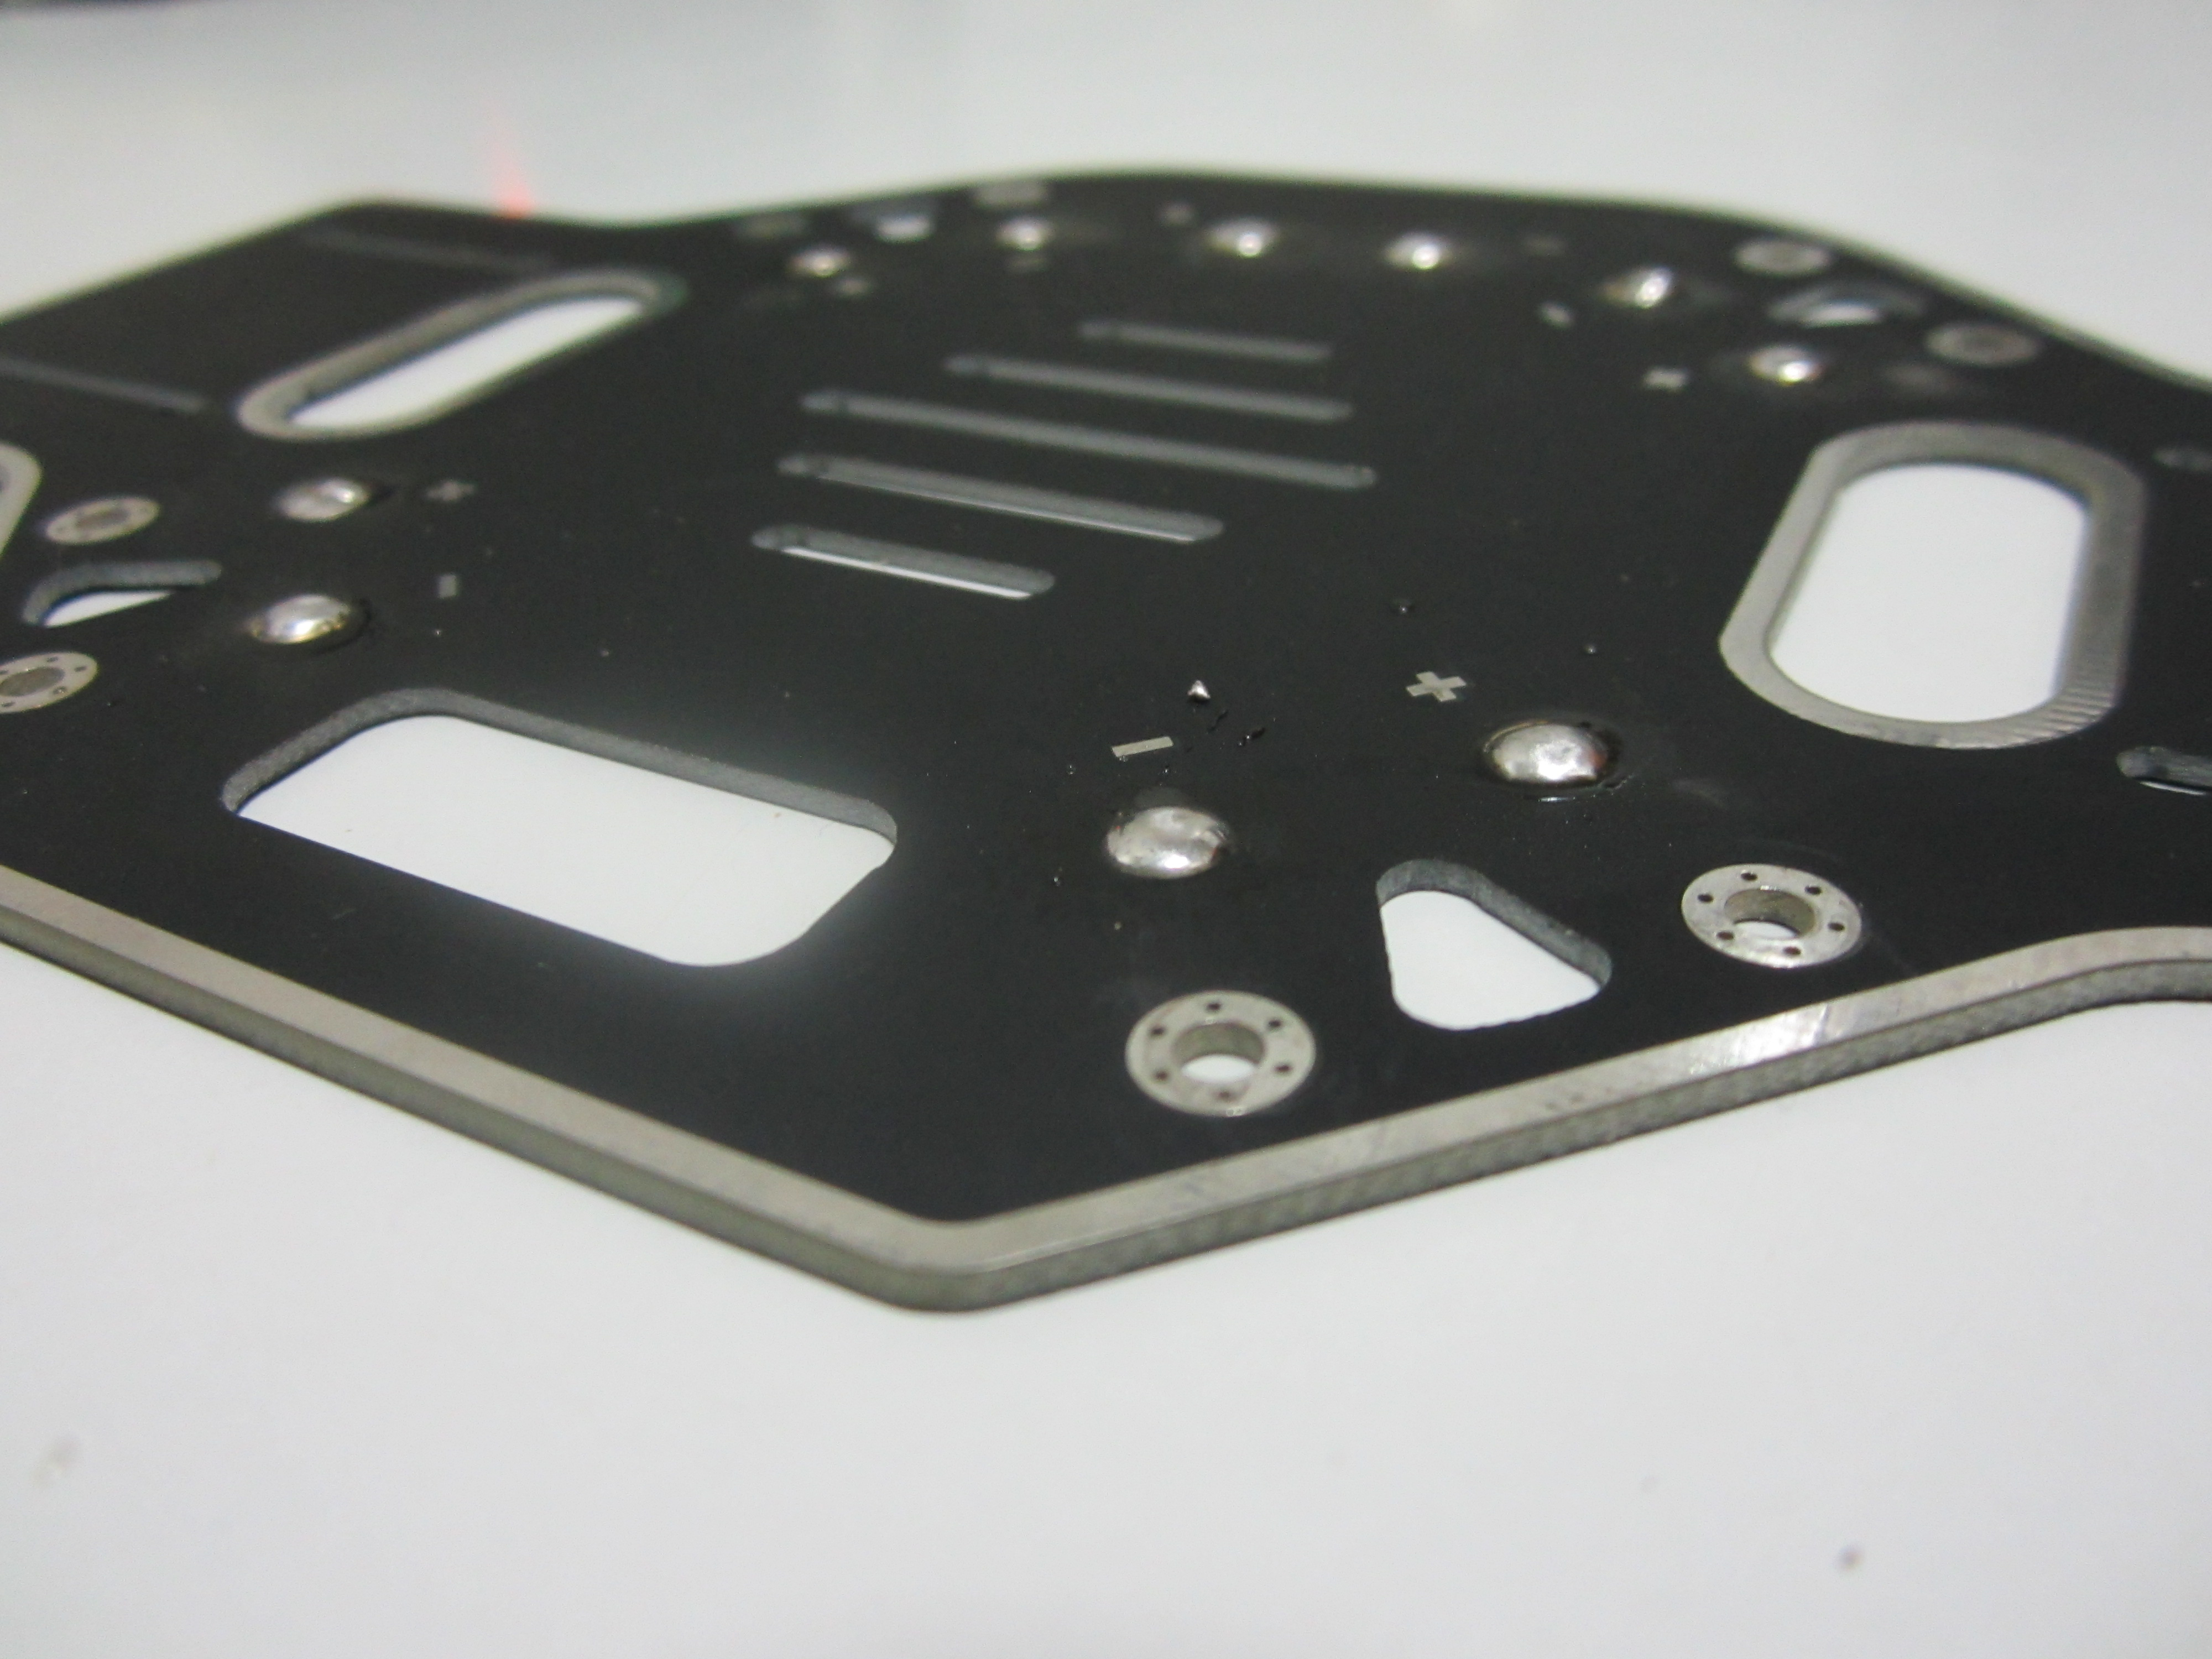
\includegraphics[width=0.8\linewidth]{Images/Mounting/IMG_0374.jpg}
  \captionof{figure}{}
  \label{fig:app2}
\end{minipage}
\\[12 pt]

\begin{minipage}{0.5\textwidth}
  \centering
  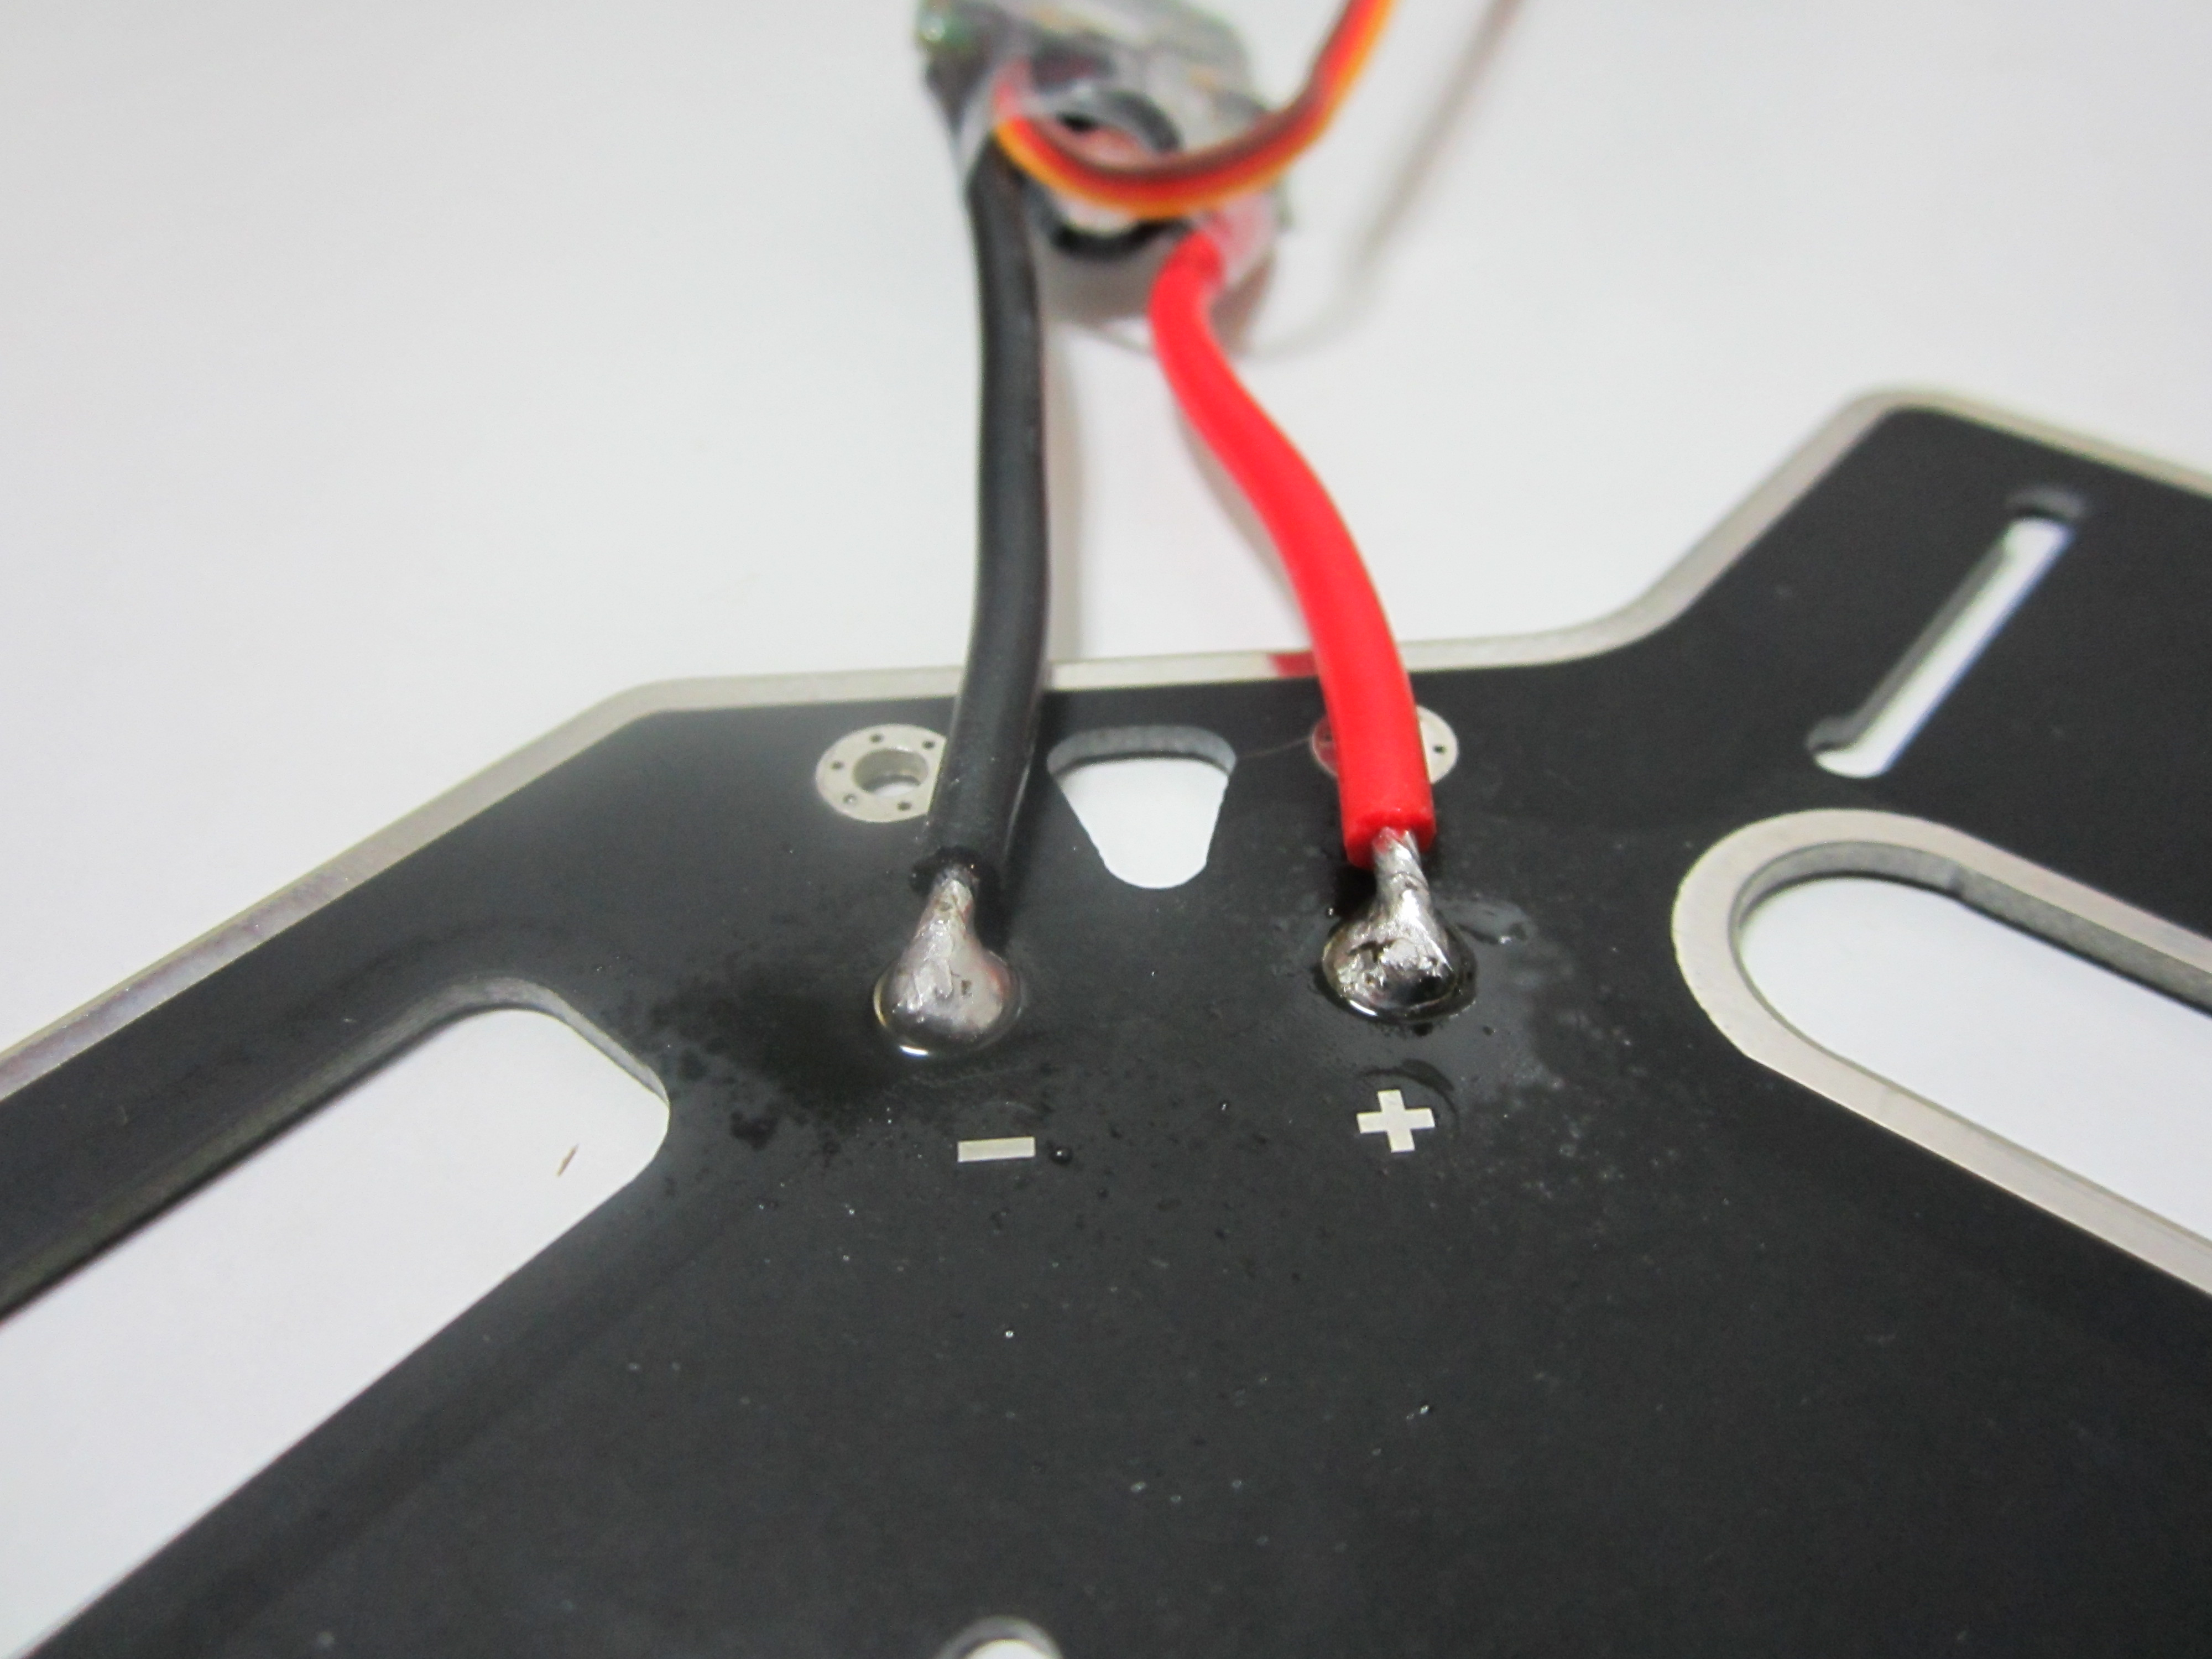
\includegraphics[width=0.8\linewidth]{Images/Mounting/IMG_0379.jpg}
  \captionof{figure}{}
  \label{fig:app1}
\end{minipage}%
\begin{minipage}{0.5\textwidth}
  \centering
  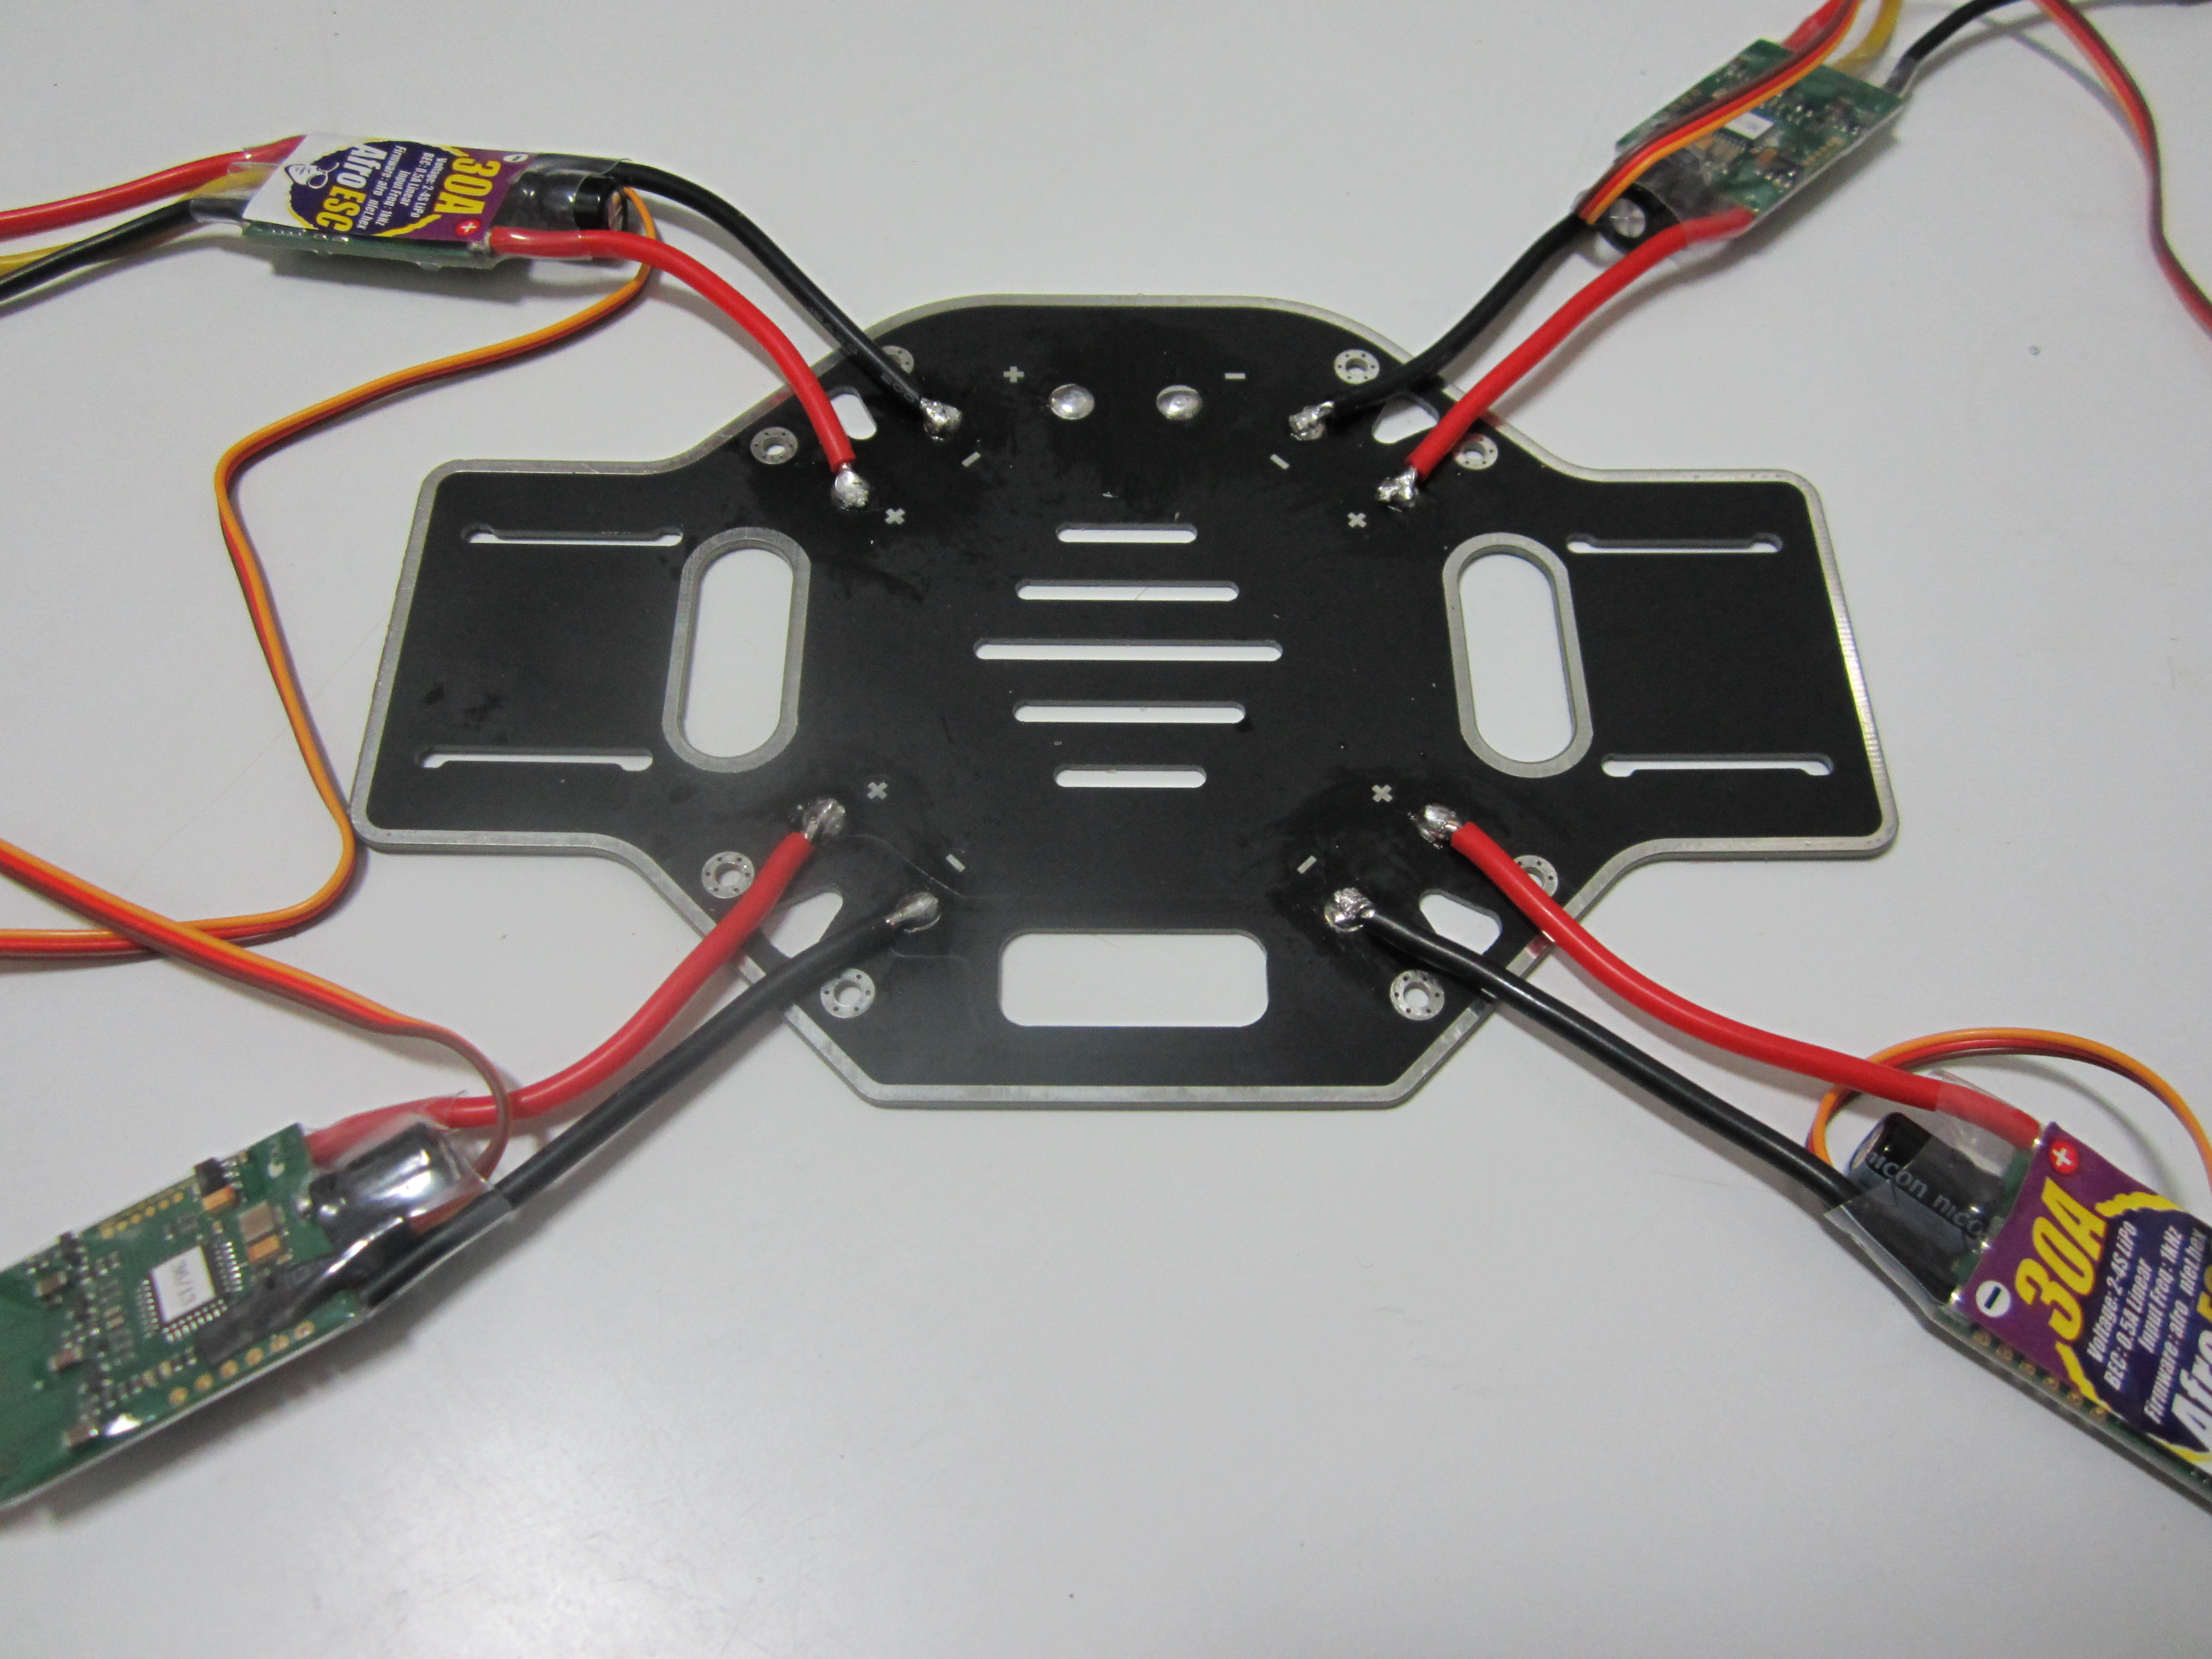
\includegraphics[width=0.8\linewidth]{Images/Mounting/IMG_0384.jpg}
  \captionof{figure}{}
  \label{fig:app2}
\end{minipage}
\\[12pt]


Once the ESCs have been soldered at the base, it is time to solder the cables that connect to the battery. These cables were purchased aside with a series of connectors compatible with the battery in order to build the necessary wiring.

To find out the length of the cable that connects to the battery is recommended to simulate the assembly of the infrastructure with the arms and putting the battery in the top base to see how this connects with the cables.
\\[12 pt]

\begin{minipage}{0.5\textwidth}
  \centering
  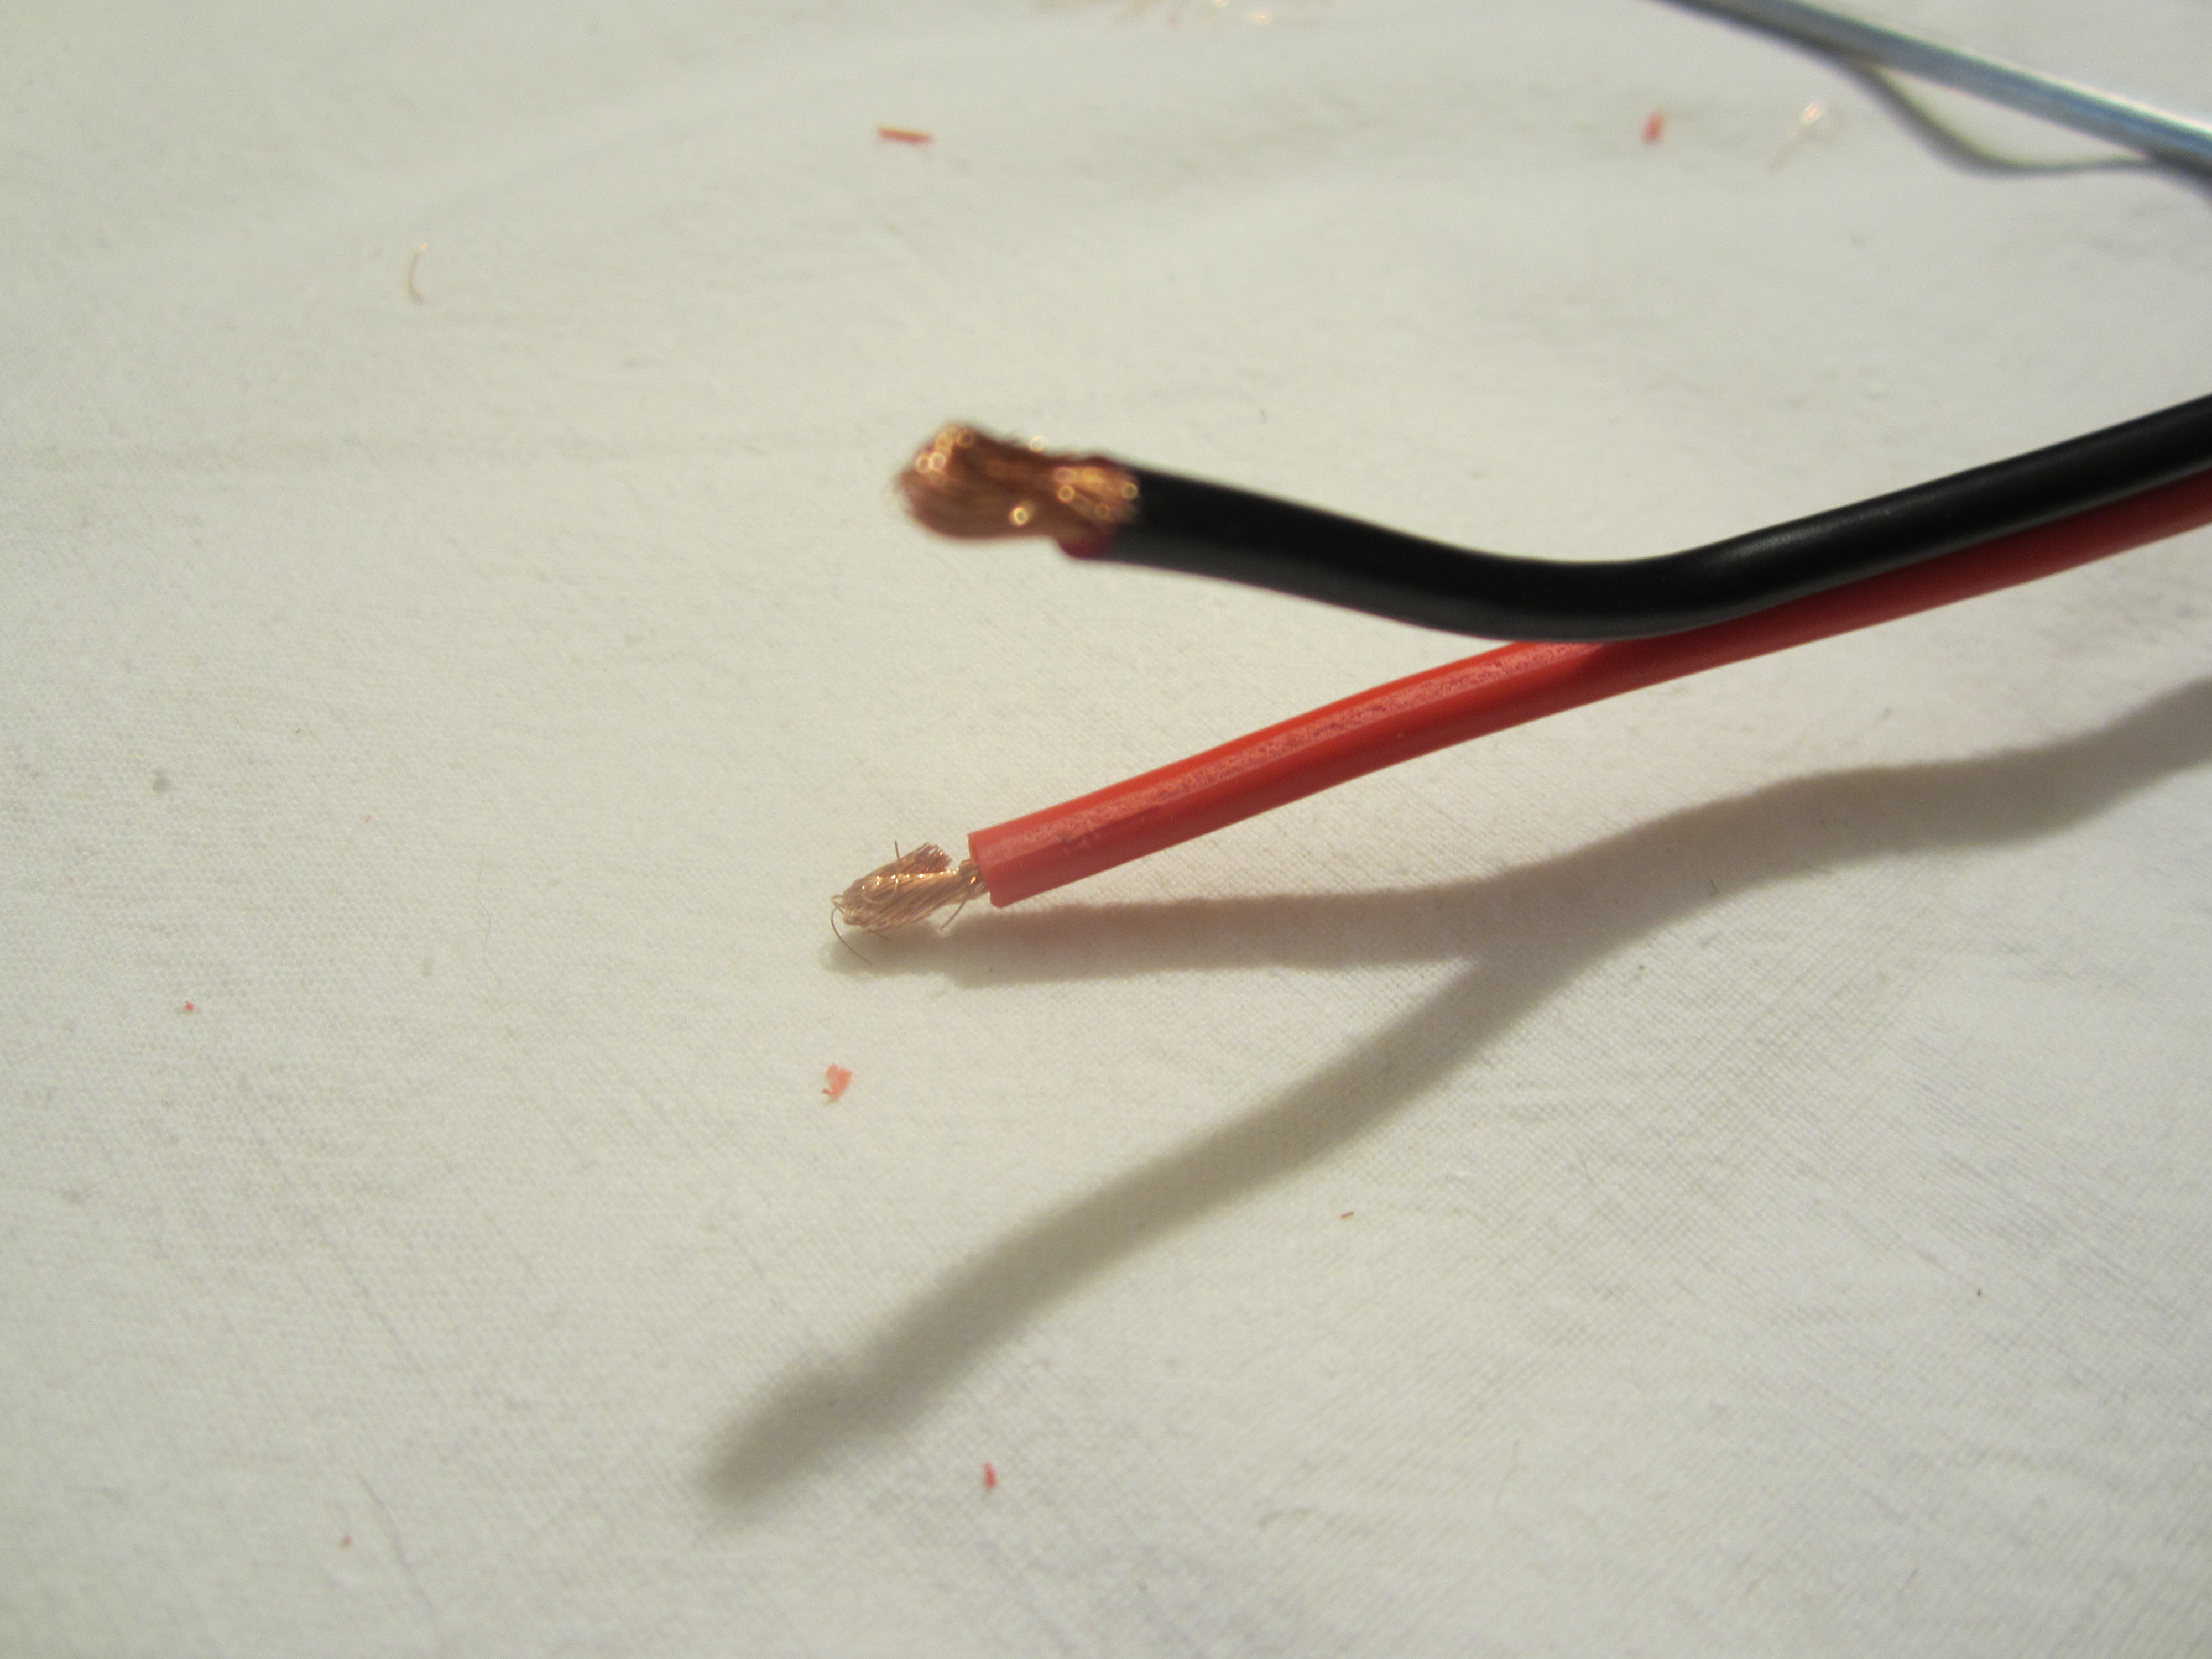
\includegraphics[width=0.8\linewidth]{Images/Mounting/IMG_0385.jpg}
  \captionof{figure}{}
  \label{fig:app1}
\end{minipage}%
\begin{minipage}{0.5\textwidth}
  \centering
  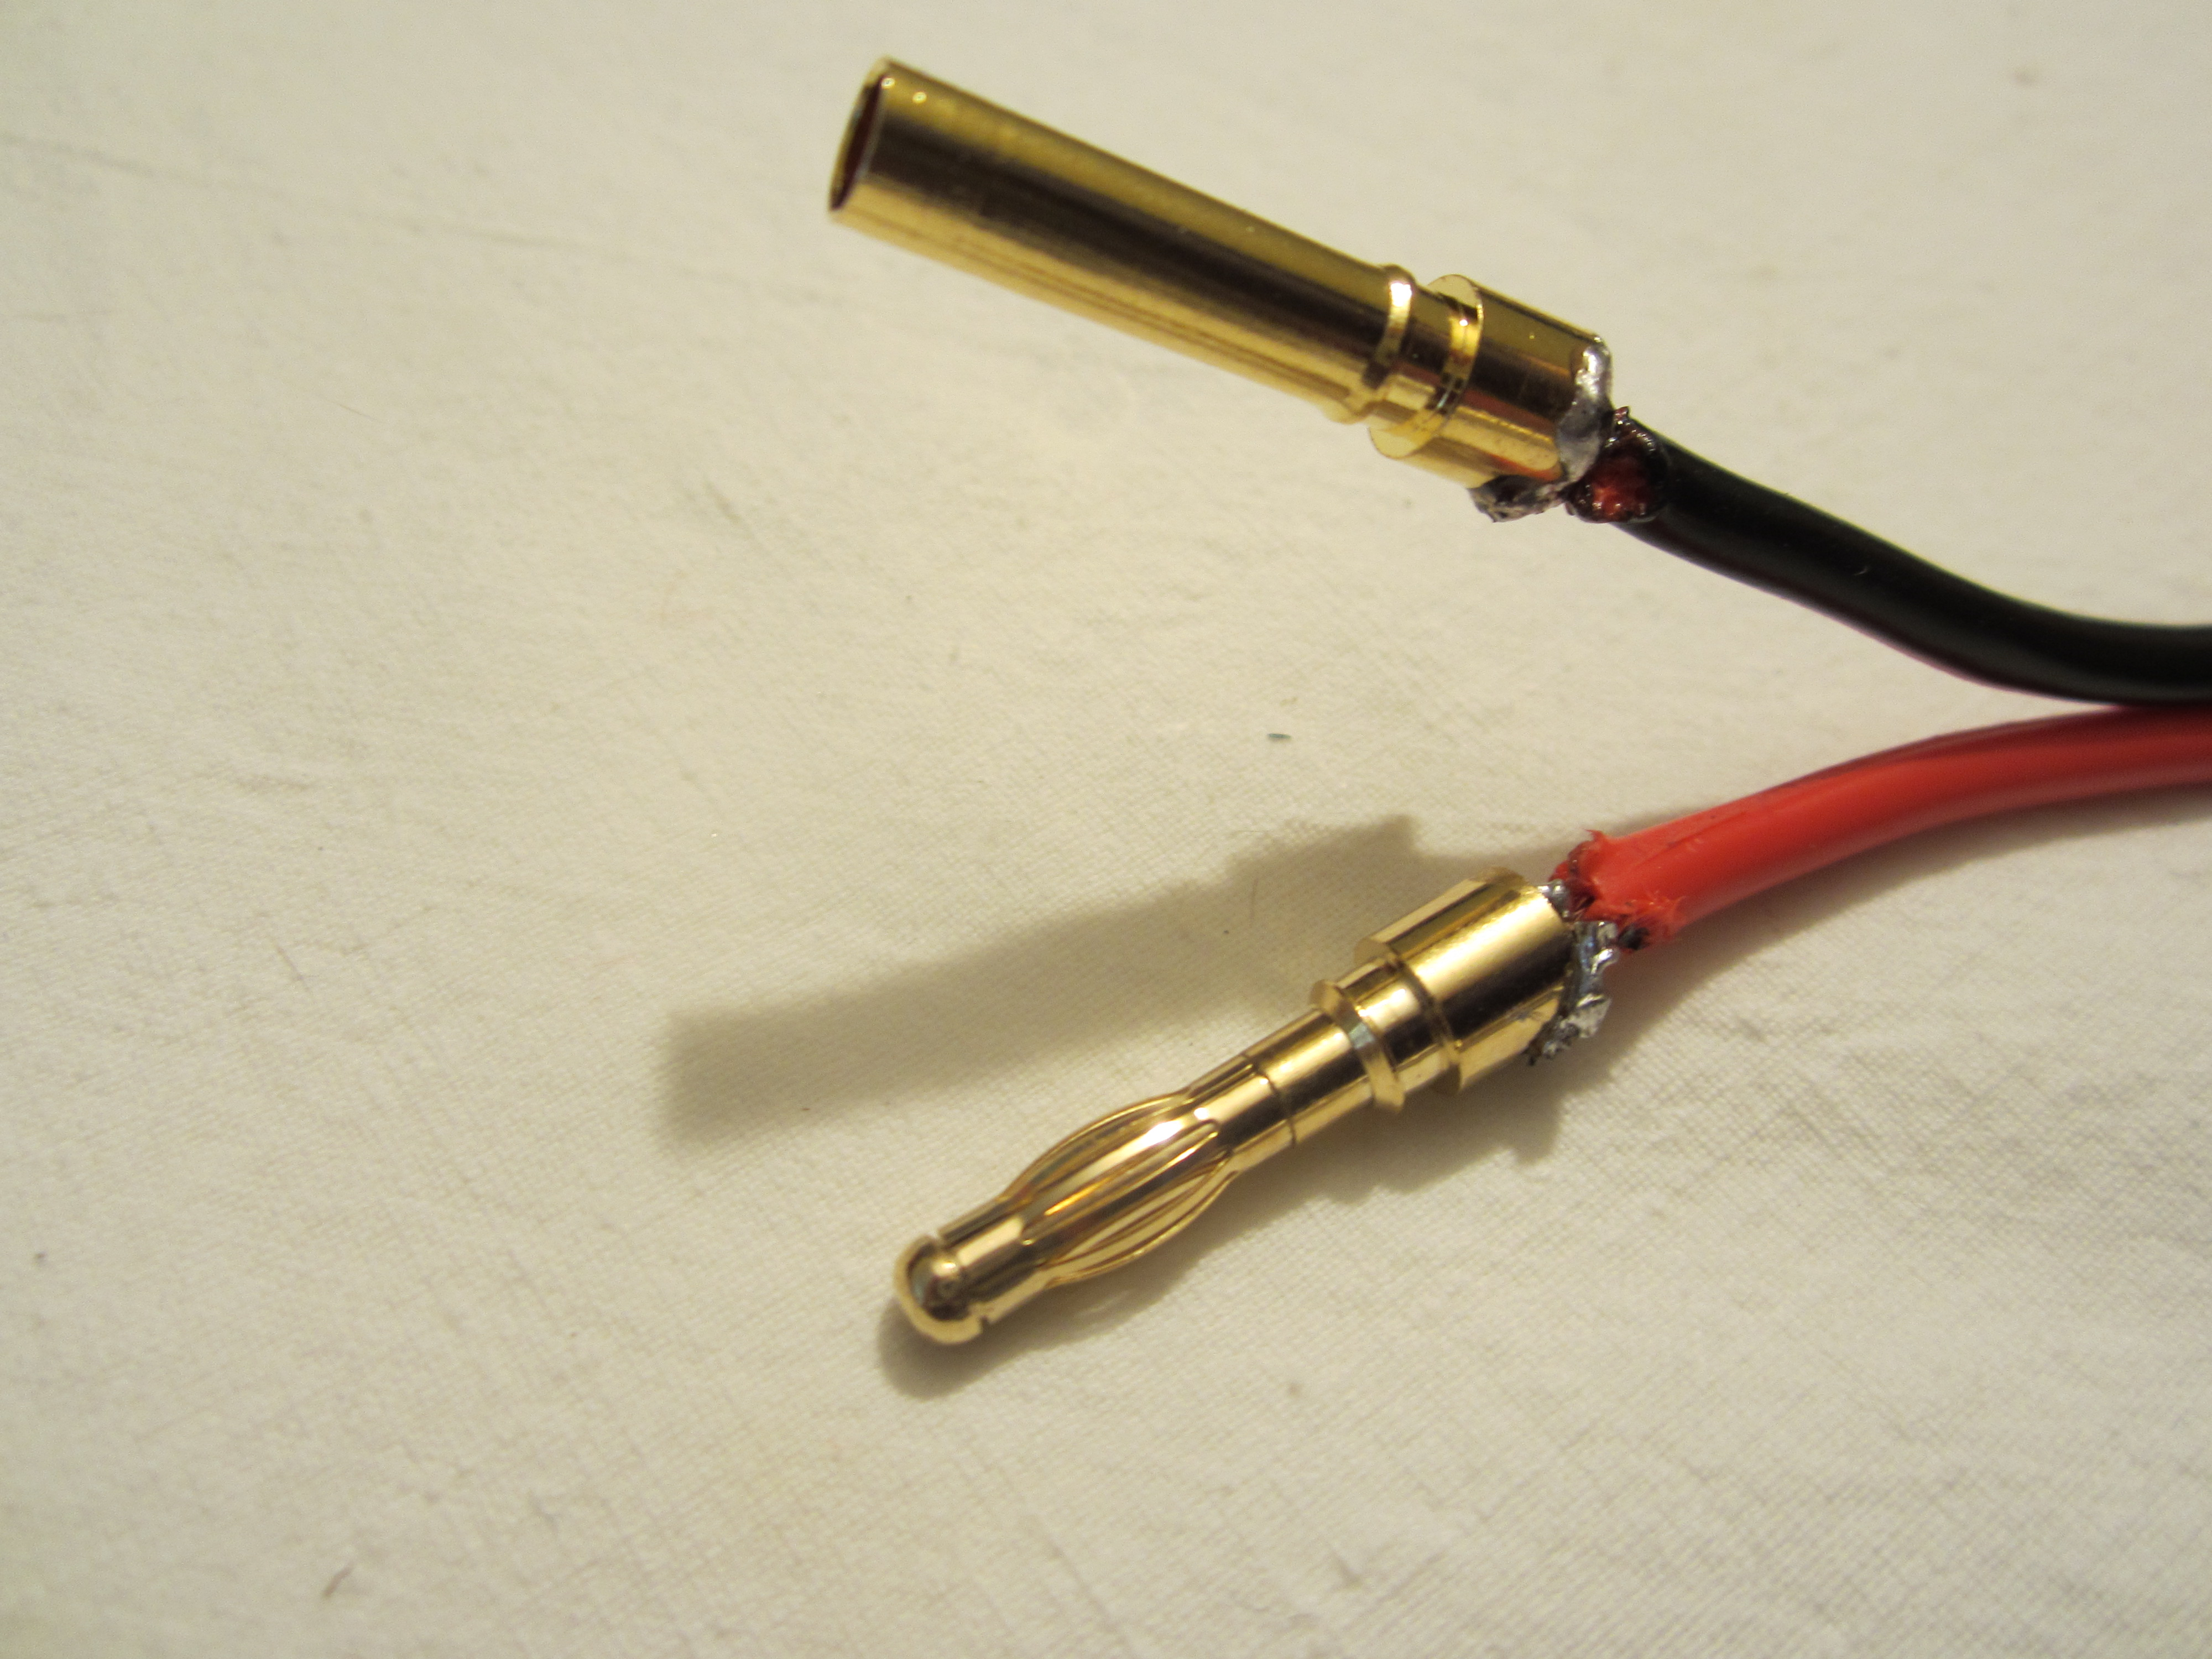
\includegraphics[width=0.8\linewidth]{Images/Mounting/IMG_0390.jpg}
  \captionof{figure}{}
  \label{fig:app2}
\end{minipage}
\\[12pt]

\begin{minipage}{0.5\textwidth}
  \centering
  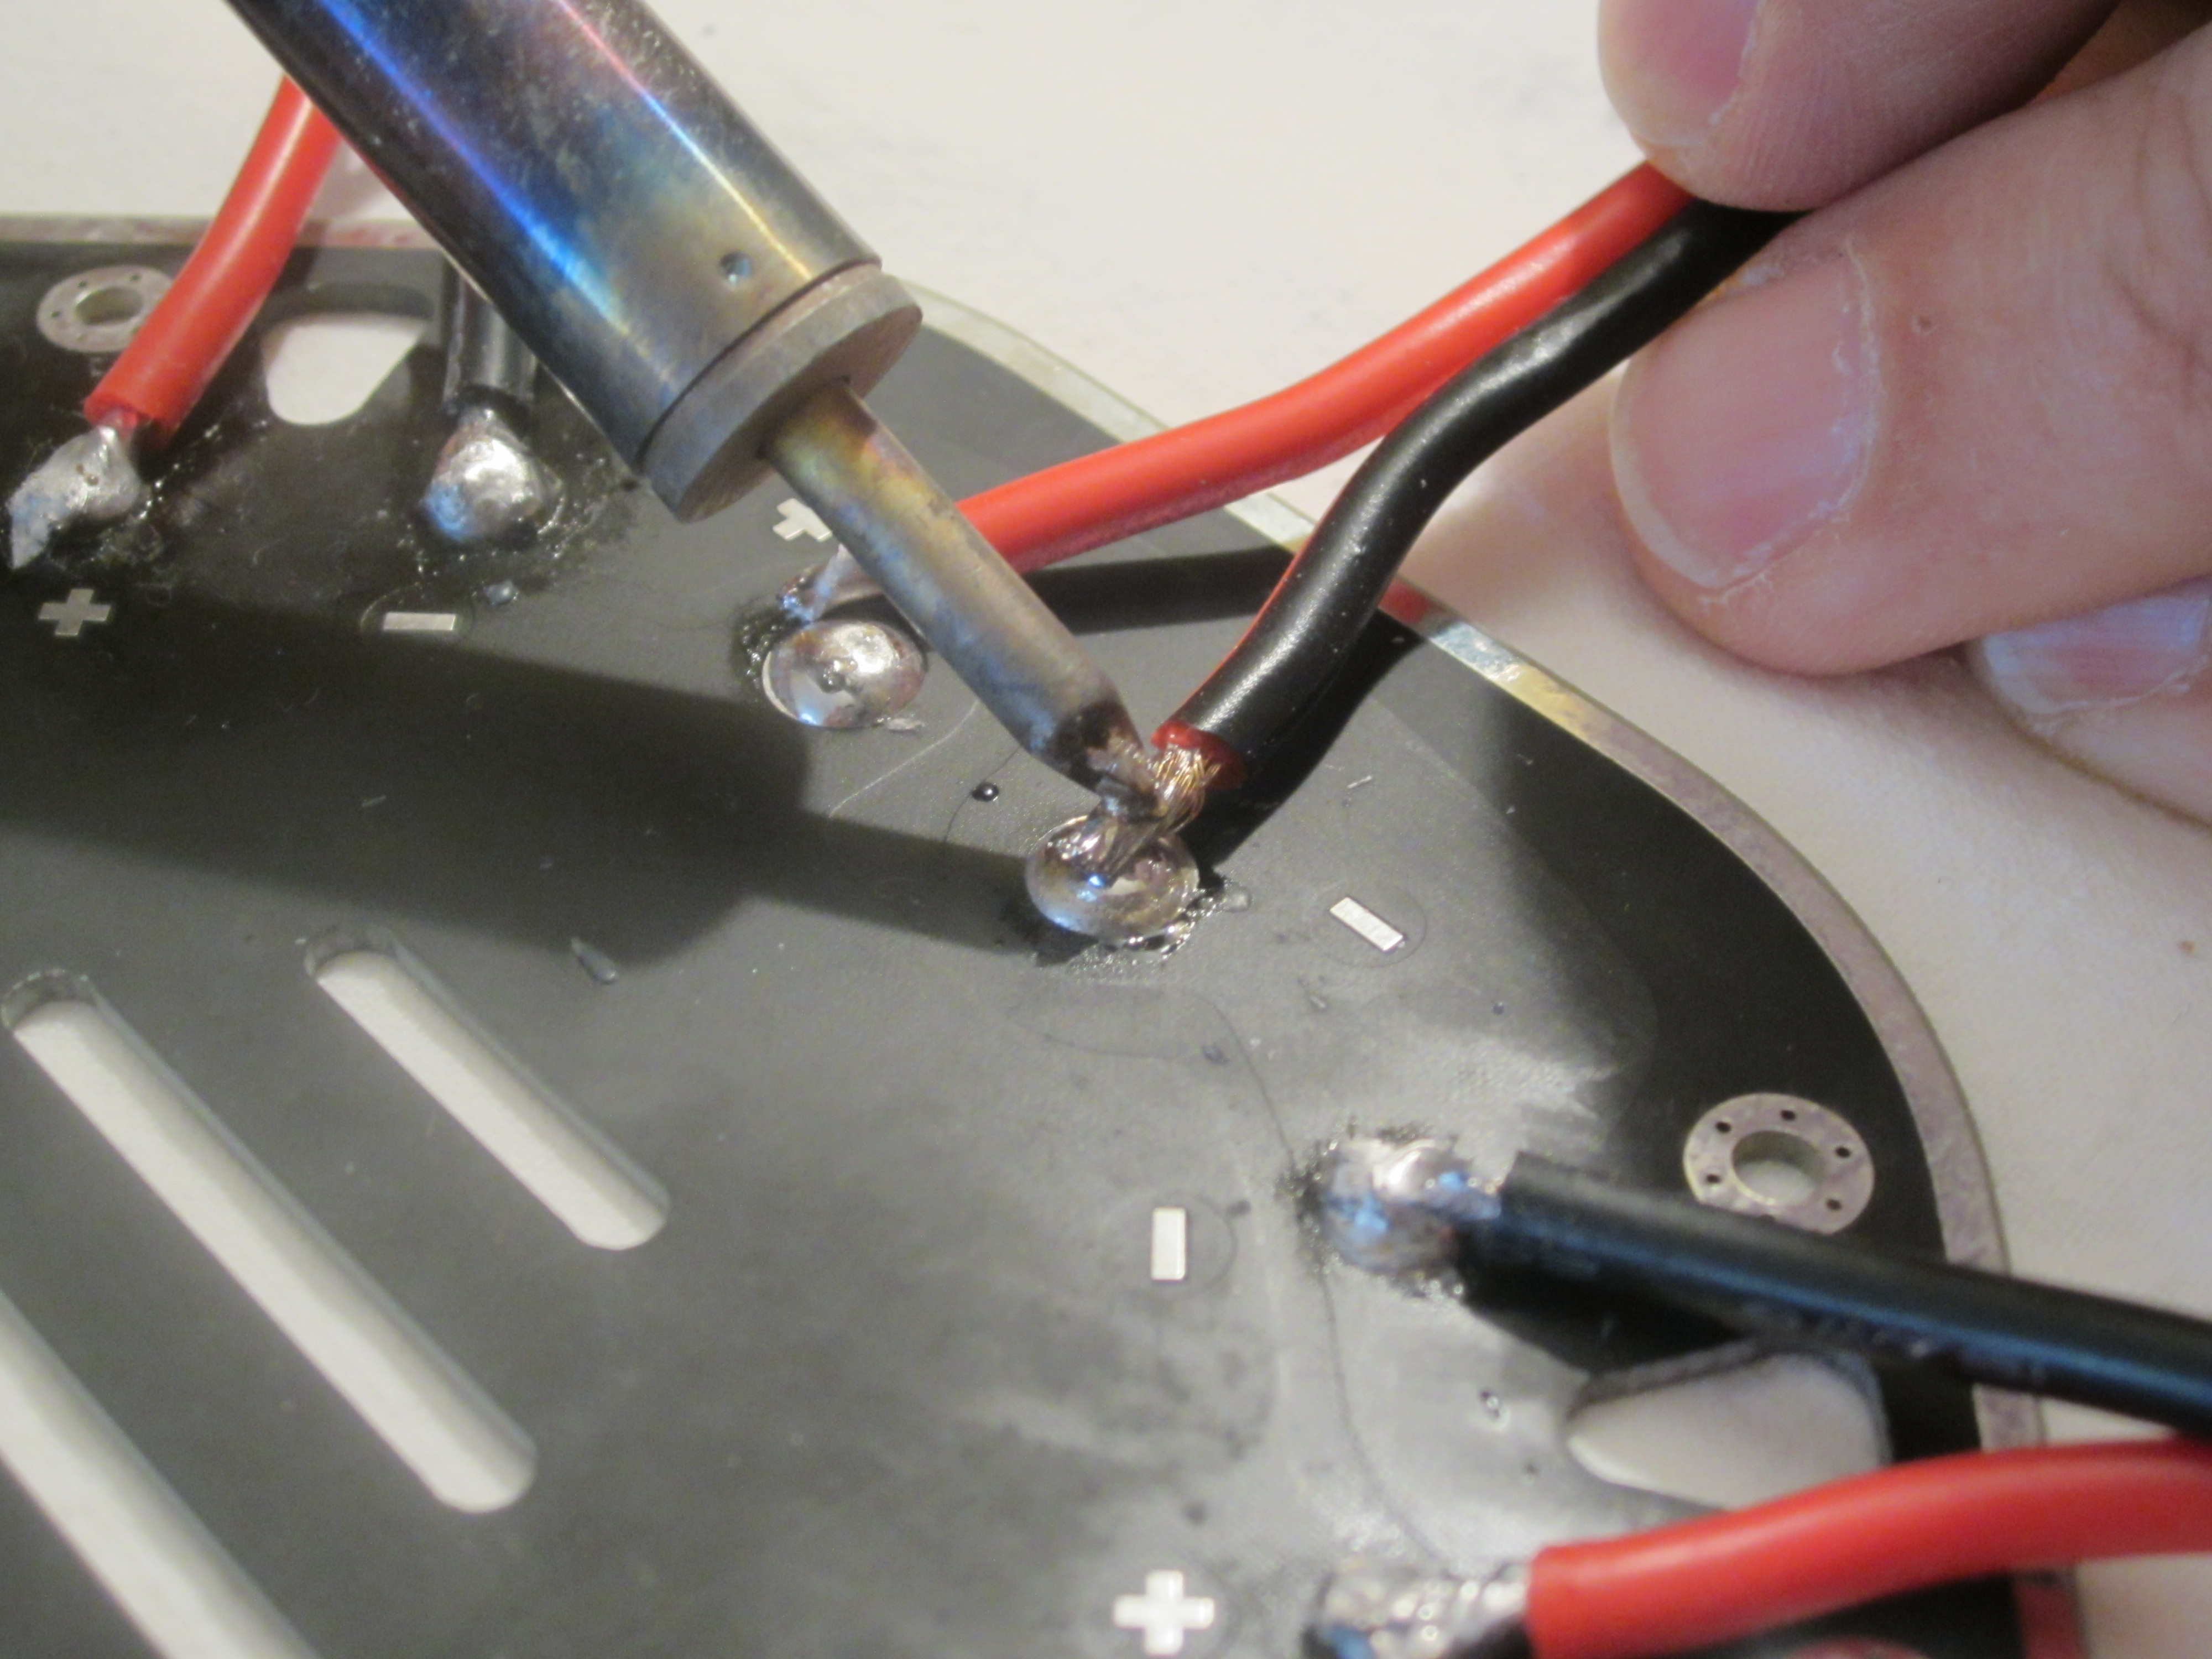
\includegraphics[width=0.8\linewidth]{Images/Mounting/IMG_0392.jpg}
  \captionof{figure}{}
  \label{fig:app1}
\end{minipage}%
\begin{minipage}{0.5\textwidth}
  \centering
  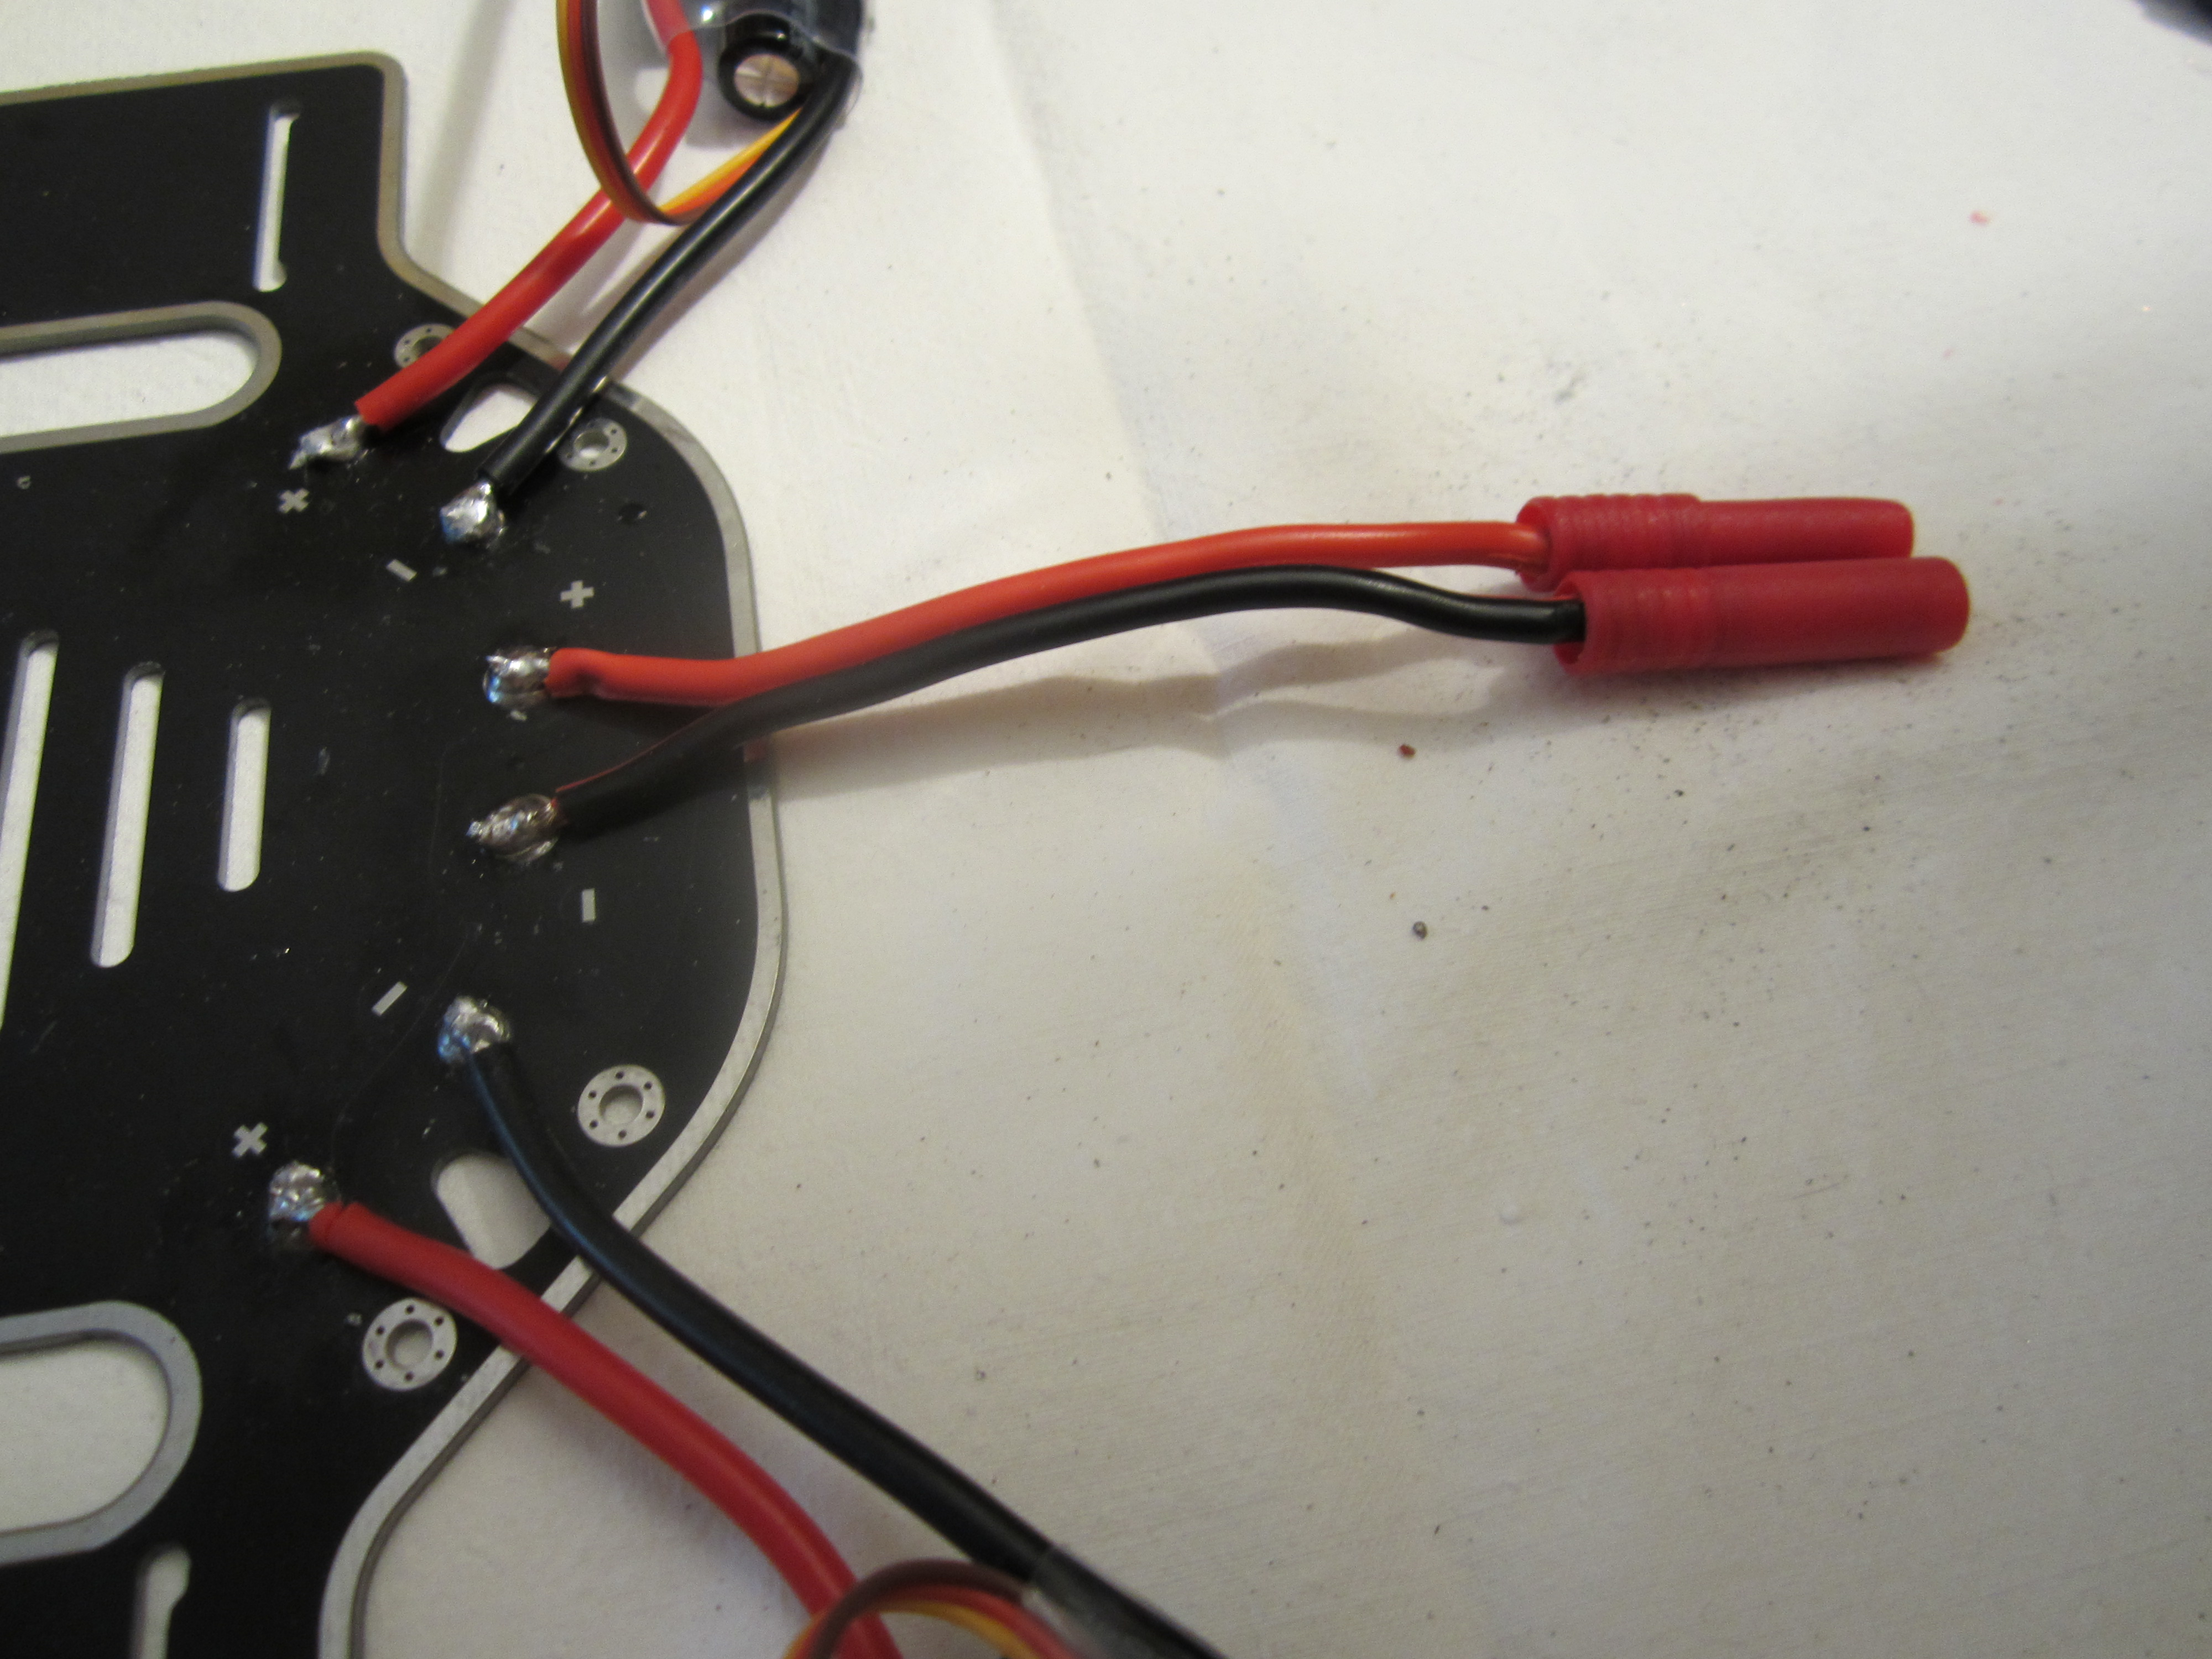
\includegraphics[width=0.8\linewidth]{Images/Mounting/IMG_0394.jpg}
  \captionof{figure}{}
  \label{fig:app2}
\end{minipage}
\\[12pt]

Once you have all the welding done, it is advisable to apply a bit of silicone with a cold gun to protect these points and avoid possible short circuits later.

\begin{minipage}{0.5\textwidth}
  \centering
  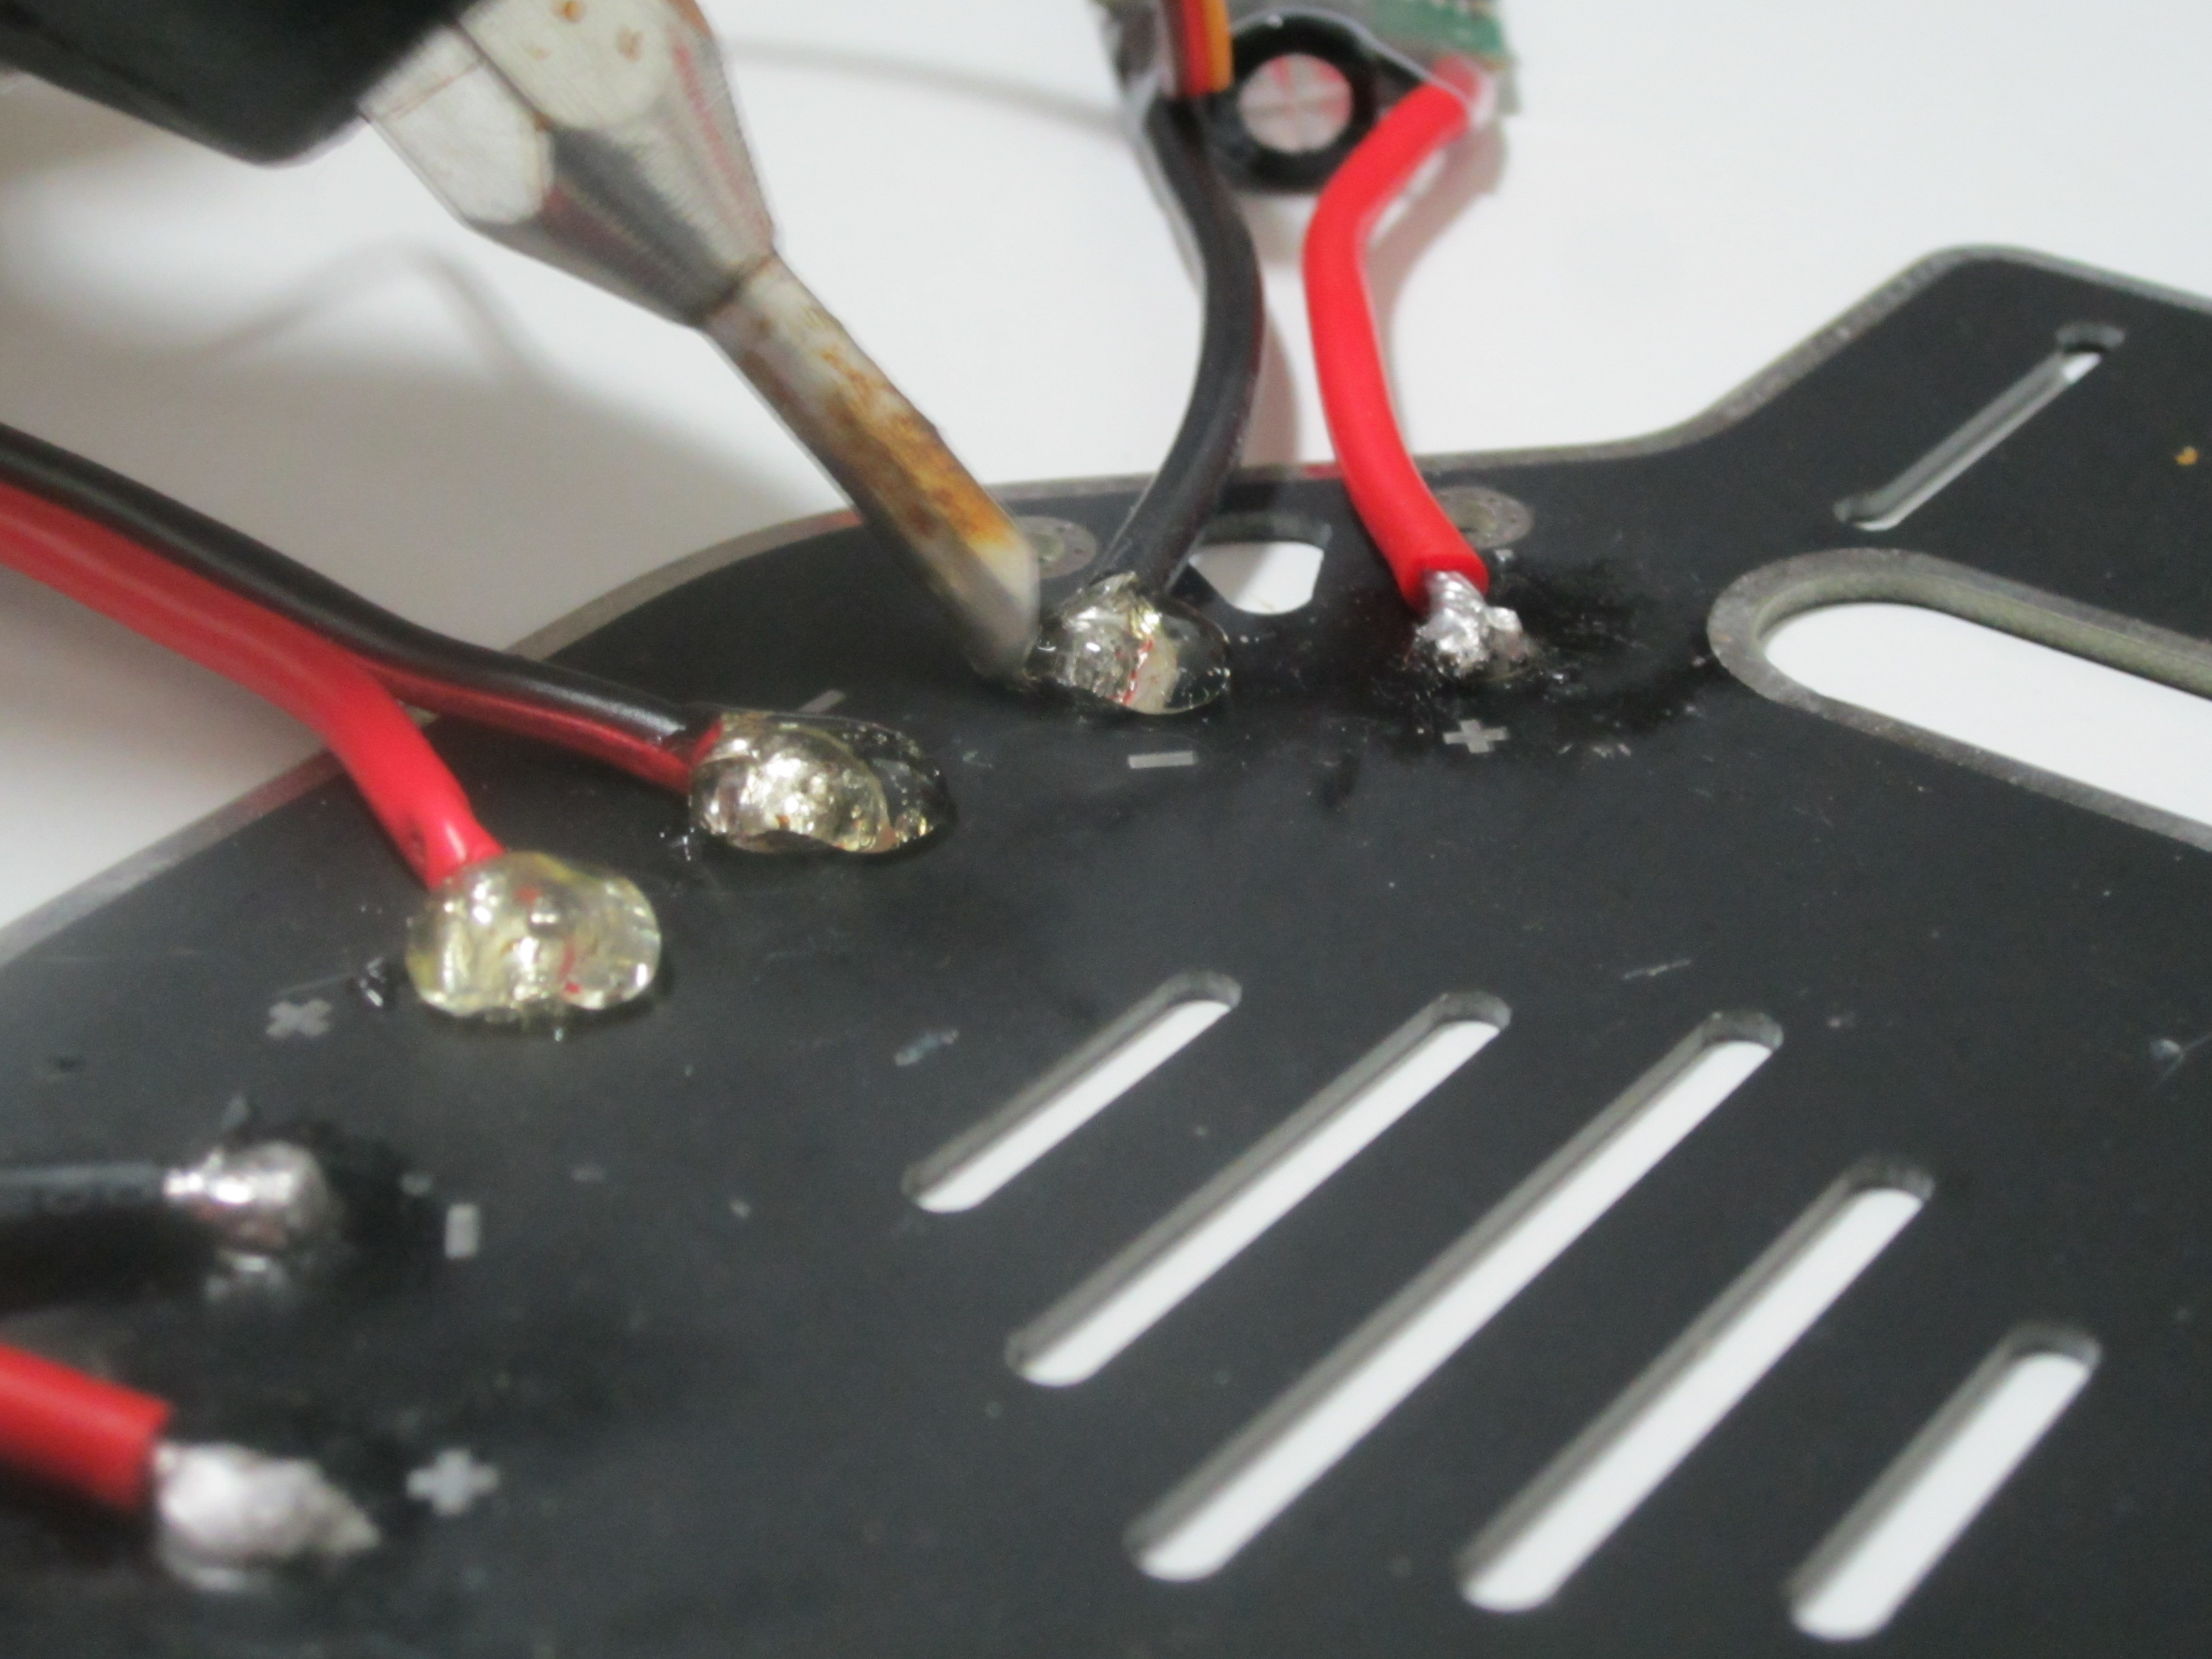
\includegraphics[width=0.8\linewidth]{Images/Mounting/IMG_0424.jpg}
  \captionof{figure}{}
  \label{fig:app1}
\end{minipage}%
\begin{minipage}{0.5\textwidth}
  \centering
  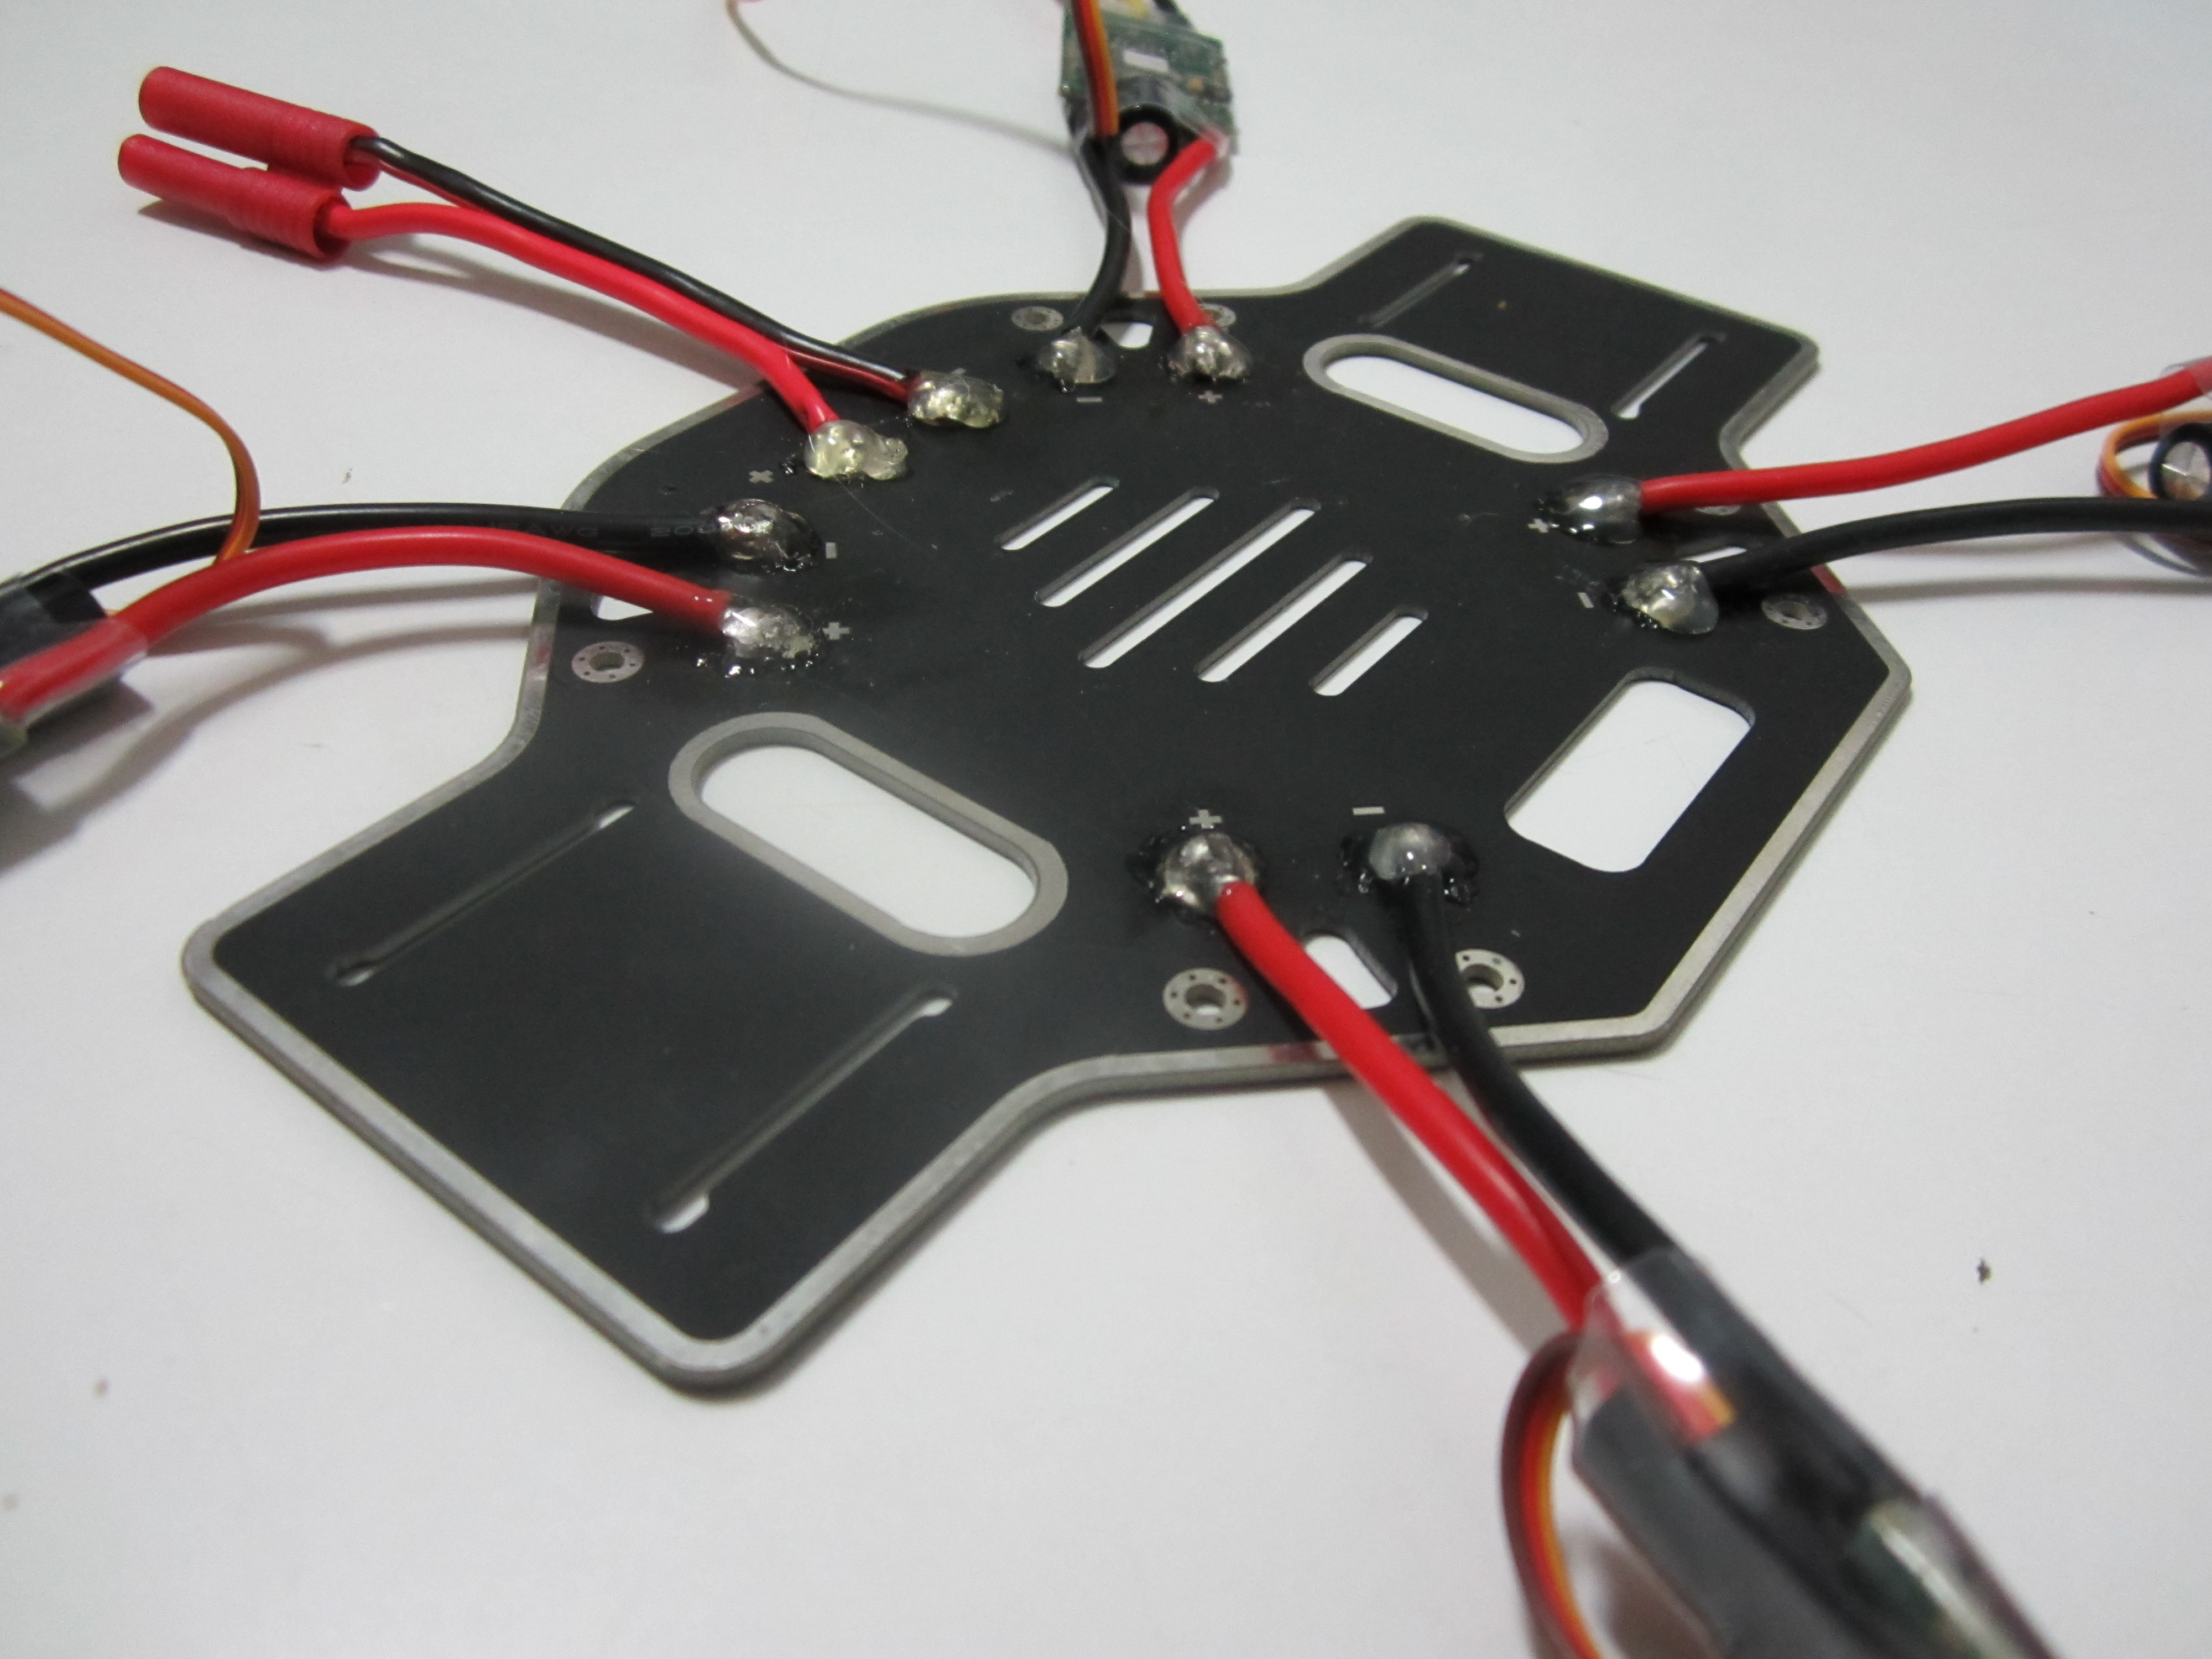
\includegraphics[width=0.8\linewidth]{Images/Mounting/IMG_0425.jpg}
  \captionof{figure}{}
  \label{fig:app2}
\end{minipage}
\\[12pt]


\section{Completion of mounting and connections}

It is important to bear in mind from now the QUAD-X figure.


%\chapter{State of the Art}

\chapter{Planning Report}

The following sections explain the tasks that I will do in the course of this project.

\section{Pieces adquisition}

This item includes the estimate time to plan which pieces are needed, how many of each, the purchase of them and the average waiting time until them arribe. 

\section{Assembling infraestructure device}

This item includes the required time to assembling the device once the pieces have arribed and we have all the needed tools.

\section{Software Implementation}

This item includes the required time to install the different software on the arduinos: the transmissor, the receptor and the controller; plus all the required software to be able to configure the arduinos through the PC.

\section{Flight Tests}

This item includes the required time to do the flight tests itself and the time to calibrate the device based on the results obtained on the tests and their interpretation.

\section{Camera incorporation}

This item includes the time needed to incorporate a camera to the device in order to take video images and transmitt it on live.

\section{Device improvements}

This item includes the required time to incorporate a bluetooth module to facilitate the connection between the arduino and the PC on a wireless mode, plus the incorporation of a GPS module, in order to extend the device possibilities.

\section{Final report}

The wording of the report is performed in parallel with the tasks that are being performed.

\section{Gantt chart}

\begin{figure}[ftbp]
  \begin{center}

    \begin{ganttchart}
    [y unit title=0.4cm, 
    y unit chart=0.5cm,
    vgrid,hgrid,
    title label anchor/.style={below=-1.6ex},
    title left shift=.05,
    title right shift=-.05,
    title height=1,
    bar/.style={fill=gray!50},
    incomplete/.style={fill=white},
    progress label text={},
    bar height=0.7,
    group right shift=0,
    group top shift=.6,
    group height=.3,
    group peaks height={}{}{.1}]{1}{24}
    
    %labels
    \gantttitle{2013-2014}{24} \\
    \gantttitle{October}{3}
    \gantttitle{November}{3} 
    \gantttitle{December}{3}
    \gantttitle{January}{3} 
    \gantttitle{February}{3} 
    \gantttitle{March}{3} 
    \gantttitle{April}{3} 
    \gantttitle{May}{3}\\
    
    %tasks
    \ganttbar{Task 1}{2}{6} \\
    \ganttbar{Task 2}{7}{12} \\
    \ganttbar{Task 3}{10}{15} \\
    \ganttbar{Task 4}{16}{24} \\
    \ganttbar{Task 5}{19}{24} \\
    \ganttbar{Task 6}{22}{24} \\
    \ganttbar{Final report}{2}{24}

    %relations 
    \ganttlink{elem0}{elem1}  
    \ganttlink{elem2}{elem3} 


   \end{ganttchart}
  \end{center}
\end{figure}




\end{document}
